% Options for packages loaded elsewhere
\PassOptionsToPackage{unicode}{hyperref}
\PassOptionsToPackage{hyphens}{url}
%
\documentclass[
]{article}
\usepackage{amsmath,amssymb}
\usepackage{iftex}
\ifPDFTeX
  \usepackage[T1]{fontenc}
  \usepackage[utf8]{inputenc}
  \usepackage{textcomp} % provide euro and other symbols
\else % if luatex or xetex
  \usepackage{unicode-math} % this also loads fontspec
  \defaultfontfeatures{Scale=MatchLowercase}
  \defaultfontfeatures[\rmfamily]{Ligatures=TeX,Scale=1}
\fi
\usepackage{lmodern}
\ifPDFTeX\else
  % xetex/luatex font selection
\fi
% Use upquote if available, for straight quotes in verbatim environments
\IfFileExists{upquote.sty}{\usepackage{upquote}}{}
\IfFileExists{microtype.sty}{% use microtype if available
  \usepackage[]{microtype}
  \UseMicrotypeSet[protrusion]{basicmath} % disable protrusion for tt fonts
}{}
\makeatletter
\@ifundefined{KOMAClassName}{% if non-KOMA class
  \IfFileExists{parskip.sty}{%
    \usepackage{parskip}
  }{% else
    \setlength{\parindent}{0pt}
    \setlength{\parskip}{6pt plus 2pt minus 1pt}}
}{% if KOMA class
  \KOMAoptions{parskip=half}}
\makeatother
\usepackage{xcolor}
\usepackage[margin=1in]{geometry}
\usepackage{color}
\usepackage{fancyvrb}
\newcommand{\VerbBar}{|}
\newcommand{\VERB}{\Verb[commandchars=\\\{\}]}
\DefineVerbatimEnvironment{Highlighting}{Verbatim}{commandchars=\\\{\}}
% Add ',fontsize=\small' for more characters per line
\usepackage{framed}
\definecolor{shadecolor}{RGB}{248,248,248}
\newenvironment{Shaded}{\begin{snugshade}}{\end{snugshade}}
\newcommand{\AlertTok}[1]{\textcolor[rgb]{0.94,0.16,0.16}{#1}}
\newcommand{\AnnotationTok}[1]{\textcolor[rgb]{0.56,0.35,0.01}{\textbf{\textit{#1}}}}
\newcommand{\AttributeTok}[1]{\textcolor[rgb]{0.13,0.29,0.53}{#1}}
\newcommand{\BaseNTok}[1]{\textcolor[rgb]{0.00,0.00,0.81}{#1}}
\newcommand{\BuiltInTok}[1]{#1}
\newcommand{\CharTok}[1]{\textcolor[rgb]{0.31,0.60,0.02}{#1}}
\newcommand{\CommentTok}[1]{\textcolor[rgb]{0.56,0.35,0.01}{\textit{#1}}}
\newcommand{\CommentVarTok}[1]{\textcolor[rgb]{0.56,0.35,0.01}{\textbf{\textit{#1}}}}
\newcommand{\ConstantTok}[1]{\textcolor[rgb]{0.56,0.35,0.01}{#1}}
\newcommand{\ControlFlowTok}[1]{\textcolor[rgb]{0.13,0.29,0.53}{\textbf{#1}}}
\newcommand{\DataTypeTok}[1]{\textcolor[rgb]{0.13,0.29,0.53}{#1}}
\newcommand{\DecValTok}[1]{\textcolor[rgb]{0.00,0.00,0.81}{#1}}
\newcommand{\DocumentationTok}[1]{\textcolor[rgb]{0.56,0.35,0.01}{\textbf{\textit{#1}}}}
\newcommand{\ErrorTok}[1]{\textcolor[rgb]{0.64,0.00,0.00}{\textbf{#1}}}
\newcommand{\ExtensionTok}[1]{#1}
\newcommand{\FloatTok}[1]{\textcolor[rgb]{0.00,0.00,0.81}{#1}}
\newcommand{\FunctionTok}[1]{\textcolor[rgb]{0.13,0.29,0.53}{\textbf{#1}}}
\newcommand{\ImportTok}[1]{#1}
\newcommand{\InformationTok}[1]{\textcolor[rgb]{0.56,0.35,0.01}{\textbf{\textit{#1}}}}
\newcommand{\KeywordTok}[1]{\textcolor[rgb]{0.13,0.29,0.53}{\textbf{#1}}}
\newcommand{\NormalTok}[1]{#1}
\newcommand{\OperatorTok}[1]{\textcolor[rgb]{0.81,0.36,0.00}{\textbf{#1}}}
\newcommand{\OtherTok}[1]{\textcolor[rgb]{0.56,0.35,0.01}{#1}}
\newcommand{\PreprocessorTok}[1]{\textcolor[rgb]{0.56,0.35,0.01}{\textit{#1}}}
\newcommand{\RegionMarkerTok}[1]{#1}
\newcommand{\SpecialCharTok}[1]{\textcolor[rgb]{0.81,0.36,0.00}{\textbf{#1}}}
\newcommand{\SpecialStringTok}[1]{\textcolor[rgb]{0.31,0.60,0.02}{#1}}
\newcommand{\StringTok}[1]{\textcolor[rgb]{0.31,0.60,0.02}{#1}}
\newcommand{\VariableTok}[1]{\textcolor[rgb]{0.00,0.00,0.00}{#1}}
\newcommand{\VerbatimStringTok}[1]{\textcolor[rgb]{0.31,0.60,0.02}{#1}}
\newcommand{\WarningTok}[1]{\textcolor[rgb]{0.56,0.35,0.01}{\textbf{\textit{#1}}}}
\usepackage{longtable,booktabs,array}
\usepackage{calc} % for calculating minipage widths
% Correct order of tables after \paragraph or \subparagraph
\usepackage{etoolbox}
\makeatletter
\patchcmd\longtable{\par}{\if@noskipsec\mbox{}\fi\par}{}{}
\makeatother
% Allow footnotes in longtable head/foot
\IfFileExists{footnotehyper.sty}{\usepackage{footnotehyper}}{\usepackage{footnote}}
\makesavenoteenv{longtable}
\usepackage{graphicx}
\makeatletter
\def\maxwidth{\ifdim\Gin@nat@width>\linewidth\linewidth\else\Gin@nat@width\fi}
\def\maxheight{\ifdim\Gin@nat@height>\textheight\textheight\else\Gin@nat@height\fi}
\makeatother
% Scale images if necessary, so that they will not overflow the page
% margins by default, and it is still possible to overwrite the defaults
% using explicit options in \includegraphics[width, height, ...]{}
\setkeys{Gin}{width=\maxwidth,height=\maxheight,keepaspectratio}
% Set default figure placement to htbp
\makeatletter
\def\fps@figure{htbp}
\makeatother
\setlength{\emergencystretch}{3em} % prevent overfull lines
\providecommand{\tightlist}{%
  \setlength{\itemsep}{0pt}\setlength{\parskip}{0pt}}
\setcounter{secnumdepth}{5}
\usepackage{booktabs}
\usepackage{amsthm}
\makeatletter
\def\thm@space@setup{%
  \thm@preskip=8pt plus 2pt minus 4pt
  \thm@postskip=\thm@preskip
}
\makeatother
\usepackage{tikz}
\usepackage{pgfplots}
\usetikzlibrary{arrows,automata,positioning}
\usepackage[utf8]{inputenc}
\usepackage[utf8]{vietnam}
\usepackage{etoolbox}
\usepackage{xcolor}
\usepackage{hyperref}
\usepackage{mathtools}
\usepackage{fontawesome5}
\makeatletter
\preto{\@verbatim}{\topsep=0pt \partopsep=-0pt}
\makeatother
\DeclareMathOperator*{\argmax}{arg\,max}
\newcommand\tstrut{\rule{0pt}{3ex}}
\newcommand\bstrut{\rule[-2.5ex]{0pt}{0pt}}
\usepackage{booktabs}
\usepackage{longtable}
\usepackage{array}
\usepackage{multirow}
\usepackage{wrapfig}
\usepackage{float}
\usepackage{colortbl}
\usepackage{pdflscape}
\usepackage{tabu}
\usepackage{threeparttable}
\usepackage{threeparttablex}
\usepackage[normalem]{ulem}
\usepackage{makecell}
\usepackage{xcolor}
\ifLuaTeX
  \usepackage{selnolig}  % disable illegal ligatures
\fi
\usepackage[]{natbib}
\bibliographystyle{apalike}
\IfFileExists{bookmark.sty}{\usepackage{bookmark}}{\usepackage{hyperref}}
\IfFileExists{xurl.sty}{\usepackage{xurl}}{} % add URL line breaks if available
\urlstyle{same}
\hypersetup{
  pdftitle={Khoa Học Dữ Liệu trong Kinh tế và Kinh doanh},
  pdfauthor={Nguyễn Quang Huy},
  hidelinks,
  pdfcreator={LaTeX via pandoc}}

\title{Khoa Học Dữ Liệu trong Kinh tế và Kinh doanh}
\author{Nguyễn Quang Huy}
\date{2024-07-18}

\begin{document}
\maketitle

{
\setcounter{tocdepth}{2}
\tableofcontents
}
\hypertarget{lux1eddi-nuxf3i-ux111ux1ea7u}{%
\section*{Lời nói đầu}\label{lux1eddi-nuxf3i-ux111ux1ea7u}}
\addcontentsline{toc}{section}{Lời nói đầu}

\hfill\break

Khoa học dữ liệu (KHDL) là ngành khoa học kết hợp giữa toán học - xác suất thống kê với khoa học máy tính và một kiến thức chuyên môn trong một lĩnh vực cụ thể như kinh tế, tài chính, y học, giáo dục, thể thao,\ldots, để khám phá những thông tin hữu ích và có giá trị nằm trong dữ liệu liên quan đến lĩnh vực chuyên môn đó. Những thông tin hữu ích này được sử dụng để hướng dẫn việc ra quyết định và lập kế hoạch chiến lược cho các cơ quan, tổ chức, doanh nghiệp và các cá nhân hoạt động trong lĩnh vực này.

Cuốn sách Khoa học dữ liệu trong Kinh tế và Kinh doanh được viết xuất phát từ nhu cầu học tập và tìm hiểu về KHDL của những bạn đọc đang học tập, nghiên cứu, và làm việc trong lĩnh vực kinh tế, quản lý, quản trị kinh doanh. Cuốn sách ít tập trung vào các khái niệm mang tính kỹ thuật trong toán học hay khoa học máy tính, mà tập trung nhiều hơn vào việc mô tả và áp dụng các phương pháp trên những vấn đề cụ thể. Trong mỗi Chương đều sẽ có phần thực hành sử dụng phần mềm thống kê R để minh họa cách triển khai các phương pháp kỹ thuật. Những phần thực hành này sẽ cung cấp cho bạn đọc những trải nghiệm thực tiễn có giá trị.

Cuốn sách phù hợp với sinh viên đại học hoặc cao học các ngành kinh tế, khoa học quản lý, quản trị kinh doanh, thương mại, tài chính ngân hàng, bảo hiểm, \ldots{} muốn nâng cao hiểu biết và tăng cường kinh nghiệm về làm việc với dữ liệu. Cuốn sách có thể làm giáo trình hoặc sách tham khảo cho một môn học kéo dài trong hai học kỳ.

Nội dung của cuốn sách bao gồm hầu hết những chủ đề quan trọng trong KHDL: thu thập dữ liệu, tiền xử lý, sắp xếp và biến đổi, trực quan hóa, và xây dựng mô hình trên dữ liệu. Các mô hình được trình bày trong cuốn sách bao gồm cả các mô hình đơn giản như hồi quy tuyến tính hay cây quyết định, và các mô hình phức tạp như mô hình tuyến tính tổng quát, mô hình cộng tính tổng quát, mô hình rừng ngẫu nhiên, học tăng cường hoặc mô hình mạng nơ-ron. Song song với trình bày và giải thích các mô hình, chúng tôi sẽ cung cấp các gói lệnh có sẵn để bạn đọc thực hành trên các dữ liệu cụ thể.

Đây là phiên bản đầu tiên của cuốn sách nên không thể tránh được những sai sót. Chúng tôi hy vọng rằng sẽ nhận được sự góp ý của bạn đọc về nội dung của cuốn sách để chúng tôi có thể hoàn thiện trong các phiên bản tiếp theo.

Xin chân thành cảm ơn các đồng nghiệp tại Khoa Toán Kinh tế nói riêng và Đại học Kinh tế Quốc dân nói chung đã đồng hành cùng với chúng tôi trong suốt quá trình hoàn thành cuốn sách này. Xin cảm ơn các thành viên của Actuarial Sciences Lab đã nỗ lực hết sức để cuốn sách này có thể đến tay người đọc trong thời gian ngắn nhất!

\begin{longtable}[]{@{}
  >{\raggedright\arraybackslash}p{(\columnwidth - 2\tabcolsep) * \real{0.5000}}
  >{\raggedright\arraybackslash}p{(\columnwidth - 2\tabcolsep) * \real{0.5000}}@{}}
\toprule\noalign{}
\endhead
\bottomrule\noalign{}
\endlastfoot
& \emph{``Gạo đem vào giã, bao đau đớn - Gạo giã xong rồi, trắng tựa bông - Sống ở trên đời, người cũng vậy - Gian nan rèn luyện mới thành công - Hồ Chí Minh.''} \\
\end{longtable}

\hypertarget{giux1edbi-thiux1ec7u-chung}{%
\section{Giới thiệu chung}\label{giux1edbi-thiux1ec7u-chung}}

\hypertarget{giux1edbi-thiux1ec7u-vux1ec1-khoa-hux1ecdc-dux1eef-liux1ec7u-vuxe0-cuxe1c-ux1ee9ng-dux1ee5ng}{%
\subsection{Giới thiệu về Khoa học dữ liệu và các ứng dụng}\label{giux1edbi-thiux1ec7u-vux1ec1-khoa-hux1ecdc-dux1eef-liux1ec7u-vuxe0-cuxe1c-ux1ee9ng-dux1ee5ng}}

Khoa học dữ liệu kết hợp giữa toán học với khoa học máy tính và một kiến thức chuyên ngành để khám phá những thông tin hữu ích và có giá trị trong dữ liệu để hỗ trợ việc ra quyết định và lập kế hoạch hành động. Một quá trình ứng dụng KHDL vào giải quyết một vấn đề cụ thể thường bao gồm các bước được mô tả như Hình @ref().

\begin{figure}

{\centering 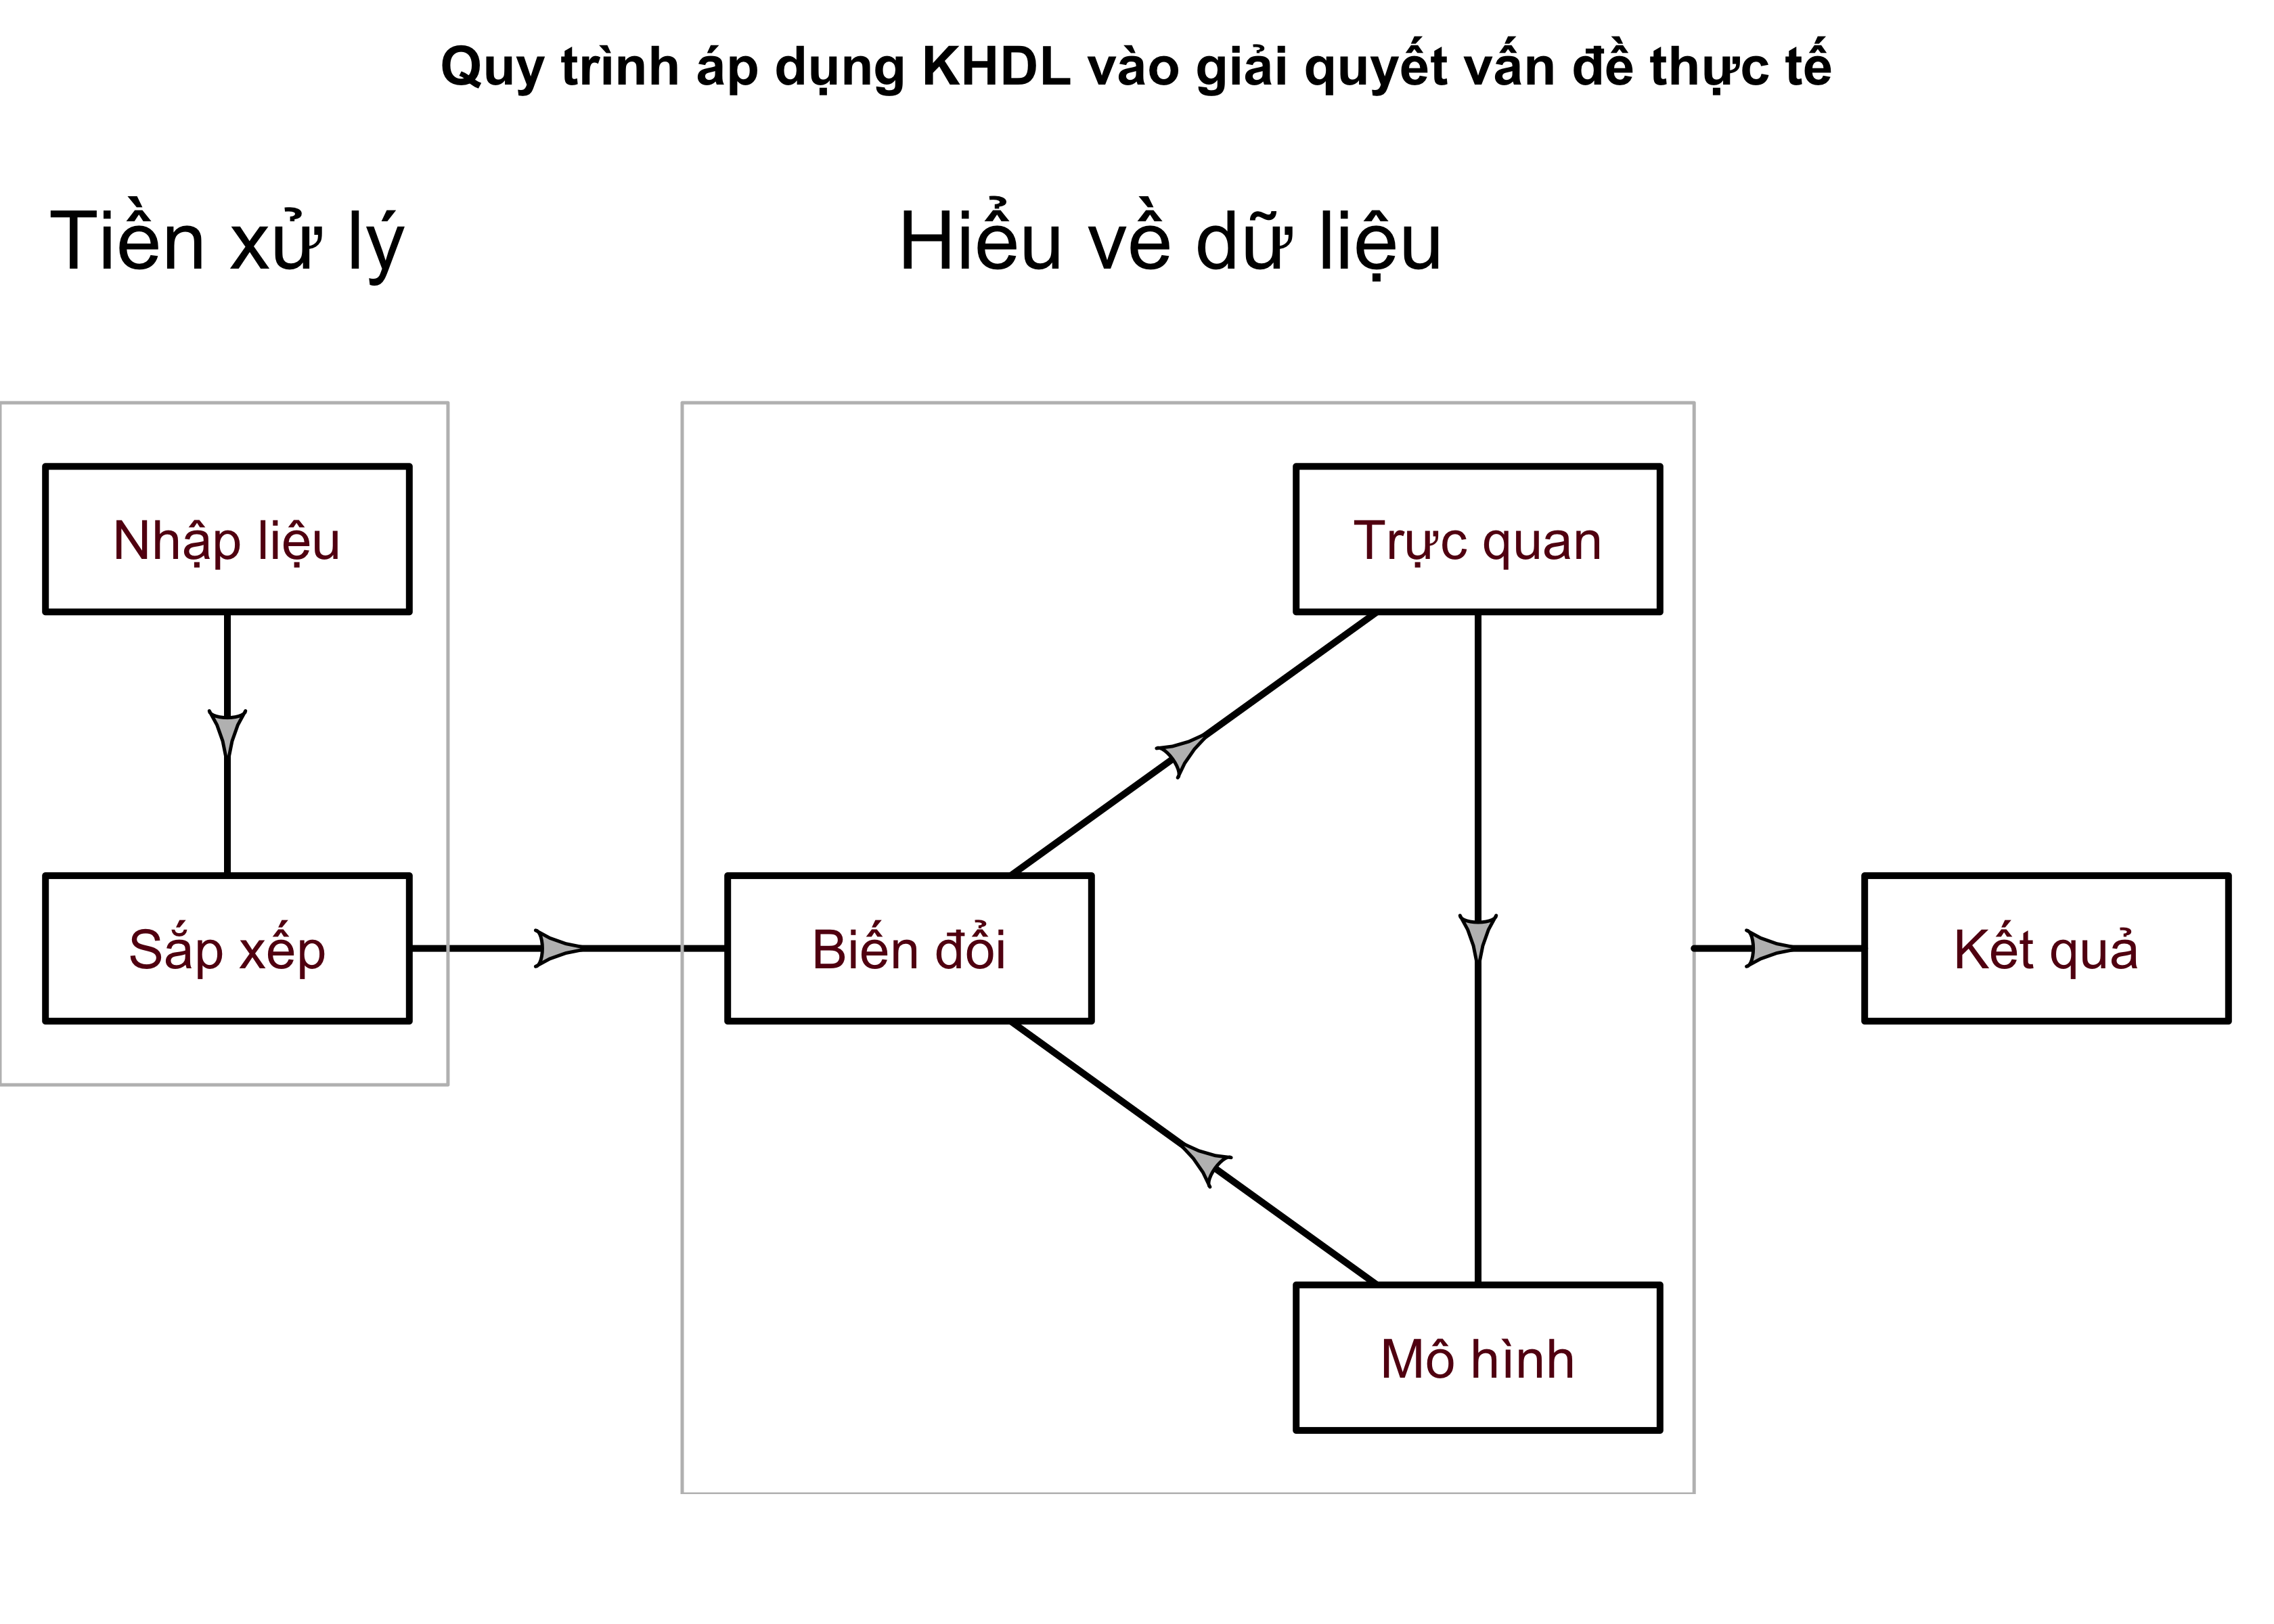
\includegraphics{01-intro_files/figure-latex/fgintro01-1} 

}

\caption{Quy trình áp dụng Khoa học dữ liệu để giải quyết một vấn đề thực tế}\label{fig:fgintro01}
\end{figure}

\begin{itemize}
\item
  \(\textbf{Nhập liệu}\) là quá trình tìm kiếm và thu thập dữ liệu từ các nguồn khác nhau để phục vụ cho mục đích ra quyết định. Có những dự án làm việc trực tiếp trên dữ liệu có sẵn và đã được thiết kế sẵn sàng cho mục tiêu phân tích nhưng cũng có những dự án mà quá trình nhập liệu lại chiếm phần lớn thời gian và quyết định sự thành công hay thất bại của dự án.
\item
  \(\textbf{Sắp xếp}\) dữ liệu hay còn được gọi là tiền xử lý dữ liệu là các bước biến dữ liệu từ dạng thô thành dữ liệu theo đúng như định dạng mong muốn.
\item
  \(\textbf{Biến đổi}\) dữ liệu là quá trình tính toán trên các biến hoặc các quan sát của dữ liệu để dữ liệu có thể đưa vào các công cụ trực quan hoặc đưa vào trong các mô hình phân tích.
\item
  \(\textbf{Xây dựng mô hình}\) là quá trình tính toán và đánh giá mối liên hệ giữa các biến trong dữ liệu đến các biến mục tiêu là đầu ra của toàn bộ quá trình. Mô hình thường được xây dựng với một trong hai mục đích là xem xét sự tác động của một biến đến các biến mục tiêu, hoặc nhằm mục đích dự đoán giá trị của các biến mục tiêu.
\end{itemize}

Mô hình trên dữ liệu được xây dựng dựa trên những nguyên lý của toán học và xác suất thống kê. Dữ liệu được sử dụng để xây dựng mô hình có thể là các dữ liệu nhỏ với một vài cột và vài chục quan sát, nhưng cũng có thể là các dữ liệu lớn với hàng nghìn cột dữ liệu và hàng triệu quan sát. Dữ liệu thậm chí không có dạng bảng biểu như chúng ta gặp hàng ngày mà có thể là các hình ảnh, các văn bản, giọng nói, dạng đồ thị, \ldots{} Để xử lý các bộ dữ liệu khổng lồ, hay các dữ liệu không có cấu trúc bảng thông thường, người xử lý dữ liệu và cần có các kiến thức về khoa học máy tính và lập trình để thực hiện các tính toán trên máy tính điện tử. Những ứng dụng của KHDL có thể thuộc về bất kỳ lĩnh vực nào như kinh doanh, y học, vật lý, thiên văn, quản lý nhà nước, chính sách công, \ldots{} nên đòi hỏi người xây dựng mô hình cũng cần có kiến thức chuyên môn trong lĩnh vực tương ứng để không bị sai định hướng trong quá trình làm việc với dữ liệu.

Để minh họa ứng dụng của KHDL trong lĩnh vực Kinh tế và Kinh doanh, chúng tôi thảo luận ngắn gọn về ba dữ liệu được thu nhập trong thế giới thực được xem xét trong cuốn sách này.

\hypertarget{dux1eef-liux1ec7u-chi-phuxed-quux1ea3ng-cuxe1o}{%
\subsubsection{Dữ liệu chi phí quảng cáo}\label{dux1eef-liux1ec7u-chi-phuxed-quux1ea3ng-cuxe1o}}

\hypertarget{dux1eef-liux1ec7u-bux1ea3o-hiux1ec3m-xe-uxf4-tuxf4}{%
\subsubsection{Dữ liệu bảo hiểm xe ô tô}\label{dux1eef-liux1ec7u-bux1ea3o-hiux1ec3m-xe-uxf4-tuxf4}}

\hypertarget{dux1eef-liux1ec7u-vux1ec1-giuxe1-nhuxe0}{%
\subsubsection{Dữ liệu về giá nhà}\label{dux1eef-liux1ec7u-vux1ec1-giuxe1-nhuxe0}}

\hypertarget{sux1a1-lux1b0ux1ee3c-quuxe1-truxecnh-phuxe1t-triux1ec3n-cux1ee7a-xuxe2y-dux1ef1ng-muxf4-huxecnh-dux1eef-liux1ec7u}{%
\subsection{Sơ lược quá trình phát triển của xây dựng mô hình dữ liệu}\label{sux1a1-lux1b0ux1ee3c-quuxe1-truxecnh-phuxe1t-triux1ec3n-cux1ee7a-xuxe2y-dux1ef1ng-muxf4-huxecnh-dux1eef-liux1ec7u}}

Mặc dù thuật ngữ xây dựng mô hình trên dữ liệu, hay được gọi một cách kỹ thuật hơn là học máy, còn khá mới mẻ nhưng những khái niệm nền tảng cho lĩnh vực này đã được phát triển từ lâu. Vào đầu thế kỷ 19, phương pháp bình phương nhỏ nhất đã được phát triển và áp dụng để ước lượng các mô hình hồi quy tuyến tính. Mô hình này lần đầu tiên được áp dụng và cho kết quả thành công trong các vấn đề liên quan đến thiên văn học. Vào đầu thế kỷ thứ 20, mô hình hồi quy tuyến tính được sử dụng để dự đoán các giá trị định lượng, chẳng hạn như mức lương của một cá nhân hoặc để dự đoán các giá trị định tính, chẳng hạn như bệnh nhân sống hay chết, hay thị trường chứng khoán tăng hay giảm. Vào những năm 1940, nhiều tác giả đã đưa ra một cách tiếp cận khác, đó là hồi quy logistic. Vào đầu những năm 1970, thuật ngữ mô hình tuyến tính tổng quát đã được phát triển để mô tả toàn bộ lớp phương pháp học thống kê bao gồm cả hồi quy tuyến tính và hồi quy logistic như các trường hợp đặc biệt. Vào cuối những năm 1970, nhiều kỹ thuật xây dựng mô hình trên dữ liệu đã xuất hiện. Tuy nhiên, các mô hình này chỉ xoay quanh là các phương pháp tuyến tính vì việc tạo ra các mối quan hệ phi tuyến tính rất khó khăn về mặt tính toán.

Đến những năm 1980, sự phát triển của máy tính điện tử đã hỗ trợ tích cực về mặt tính toán cho các các phương pháp phi tuyến tính. Các mô hình phi tuyến được giới thiệu vào đầu những năm của thập niên 80 bao gồm có mô hình cây quyết định và mô hình cộng tính tổng quát. Những năm cuối thập niên 80 và đầu thập niên 90, mô hình mạng nơ-ron được giới thiệu đến cộng đồng nghiên cứu nhưng chưa có được nhiều sự quan tâm vì dữ liệu chưa đủ phong phú và sự phổ biến của các mô hình học máy khác.

Giai đoạn cuối thế kỷ XX và đầu thế kỷ XXI là giai đoạn chiếm ưu thế hoàn toàn của các mô hình học máy rừng ngẫu nhiên và thuật toán học tăng cường. Thuật toán học tăng cường với các biến thể như XGBoost hay LightGBM chiến thắng trong hầu hết các cuộc thi về Khoa học dữ liệu.

Từ năm 2010, với sự bùng nổ của các thiết bị thông minh và kết nối internet, dữ liệu trở nên phong phú và đa dạng hơn cũng là thời điểm quay trở lại của mô hình mạng nơ-ron, hay còn được gọi với tên gọi khác là mô hình mạng học sâu (deep learning). Mô hình mạng học sâu vượt trội hoàn toàn các mô hình học máy thông thường khi làm việc với dữ liệu kiểu hình ảnh, video, ngôn ngữ tự nhiên bao gồm cả văn bản và giọng nói. Sự kiện đánh dấu sự phát triển vượt bậc của các mô hình mạng học sâu là sự ra đời của ChatGPT vào cuối những năm 2022 là một mô hình ngôn ngữ lớn cho phép người dùng tương tác, hỏi đáp và trò chuyện một cách hoàn toàn tự nhiên theo định hướng của người sử dụng như phong cách, mức độ chi tiết, hình thức ngôn ngữ. ChatGPT nhanh chóng đạt đến 100 triệu người sau hơn hai tháng phát hành và giúp cho công ty phát hành OpenAI được định giá khoảng 30 tỷ USD. Cho đến thời điểm cuối năm 2023 khi nhóm tác giả bắt đầu viết cuốn sách này, ChatGPT đã được cập nhật đến phiên bản 3.5.

\hypertarget{tux1ea1i-sao-lux1ea1i-sux1eed-dux1ee5ng-phux1ea7n-mux1ec1m-r}{%
\subsection{Tại sao lại sử dụng phần mềm R}\label{tux1ea1i-sao-lux1ea1i-sux1eed-dux1ee5ng-phux1ea7n-mux1ec1m-r}}

Trong thế giới ngày nay, hầu hết các cơ quan, tổ chức, tập đoàn, doanh nghiệp từ lớn đến nhỏ đều sử dụng một số lượng dữ liệu nhất định để phân tích các sự kiện trong quá khứ và cố gắng dự đoán xu hướng trong tương lai để đưa ra các quyết định có lợi cho mình. Tuy nhiên khi dữ liệu ngày càng tăng lên cả về số lượng và sự phức tạp, thì các cơ quan tổ chức cần một công cụ giúp họ thực hiện được các phân tích trên dữ liệu một cách nhanh hơn và chính xác hơn. Một trong các công cụ hiệu quả nhất tại thời điểm hiện tại là phần mềm R.

\hypertarget{phux1ea7n-mux1ec1m-r-luxe0-guxec}{%
\subsubsection{Phần mềm R là gì?}\label{phux1ea7n-mux1ec1m-r-luxe0-guxec}}

Trước tiên, R là ngôn ngữ lập trình được xây dựng để phục vụ cho toán học và thống kê, đồng thời R cũng là một môi trường phần mềm mã nguồn mở miễn phí cho người sử dụng. R được giới thiệu lần đầu tiên vào năm 1992 bởi các giáo sư Ross Ihaka và Robert Gentleman như một ngôn ngữ lập trình để dạy thống kê tại Đại học Auckland. Tên của ngôn ngữ, R, xuất phát từ chữ cái đầu tiên của các tác giả là Ross và Robert.

Trước khi trở thành ngôn ngữ lập trình cho Khoa học dữ liệu, R thường được coi là ngôn ngữ lập trình cho các nhà toán học và thống kê. Sau nhiều năm phát triển, R luôn được coi vẫn là một trong những ngôn ngữ lập trình phổ biến nhất trong giới học thuật vì độ tin cậy. Mỗi thư viện của R đều được phát triển một cách hoàn chỉnh và trải qua quá trình kiểm soát chặt chẽ. Tạp chí R (R Journal) là tạp chí học thuật về các phương pháp tính toán trong toán học và thống kê sử dụng phầm mềm R luôn trong danh sách các tạp chí khoa học uy tín (Science Citation Index Expanded hay SCIE) của Web of Science. Chính vì sự uy tín trong học thuật nên đa số các trường đại học và viện nghiên cứu hàng đầu trên thế giới sử dụng như là một ngôn ngữ chính trong đào tạo về tính toán, toán học và thống kê.

\hypertarget{tux1ea1i-sao-r-lux1ea1i-ux111ux1b0ux1ee3c-sux1eed-dux1ee5ng-trong-khdl}{%
\subsubsection{Tại sao R lại được sử dụng trong KHDL}\label{tux1ea1i-sao-r-lux1ea1i-ux111ux1b0ux1ee3c-sux1eed-dux1ee5ng-trong-khdl}}

Trong khoảng hơn 10 năm trở lại đây, R không còn chỉ là ngôn ngữ lập trình thông thường như trước đây nữa. Mặc dù vẫn là một công cụ mạnh mẽ trong tính toán toán học và thống kê, nhưng còn có rất nhiều công cụ tuyệt vời khác mà bạn đọc có thể làm với R, đặc biệt là những ứng dụng trong KHDL. Nguyên nhân chính giúp cho phần mềm R nhanh chóng trở thành ngôn ngữ phổ biến trong KHDL là do nền tảng quan trọng nhất của KHDL chính là toán học và thống kê. Đồng thời, ngôn ngữ lập trình R cũng đủ linh hoạt để người sử dụng viết các chương trình yêu cầu tính toán phức tạp trong Khoa học máy tính. Một cách tự nhiên, những nhà toán học, thống kê học và các tổ chức sử đang dụng R như là một ngôn ngữ chính sẽ tìm cách phát triển R để đáp ứng được với yêu cầu xử lý dữ liệu của chính họ. Một nguyên nhân khác khiến cho R phổ biến trong KHDL là do đặc thù mã nguồn mở của phần mềm này. Những người làm việc trong lĩnh vực KHDL sử dụng R có thể chia sẻ kiến thức và kinh nghiệm một cách nhanh chóng và rộng rãi.

\hypertarget{r-cuxf3-thux1ec3-luxe0m-nhux1eefng-guxec}{%
\subsubsection{R có thể làm những gì?}\label{r-cuxf3-thux1ec3-luxe0m-nhux1eefng-guxec}}

Danh sách những việc bạn có thể làm trong R là không thể liệt hết bởi vì phần mềm này vẫn đang được phát triển không ngừng. Dưới đây là một số ứng dụng phổ biến mà R vượt trội hơn so với các ngôn ngữ khác:

\begin{itemize}
\item
  Lập trình trong toán học, tính toán tối ưu, giải tối ưu bằng phương pháp số
\item
  Tính toán liên quan đến lý thuyết xác suất.
\item
  Thực hiện các kiểm định thống kê.
\item
  Phát triển phần mềm thống kê.
\item
  Xây dựng mô hình kinh tế lượng.
\item
  Mô phỏng ngẫu nhiên.
\end{itemize}

Các tính năng của R dành cho Khoa học dữ liệu được liệt kê dưới đây:

\begin{itemize}
\item
  Thu thập tập dữ liệu, bao gồm cả dữ liệu lớn và không có cấu trúc,
\item
  Khai phá dữ liệu,
\item
  Xử lý, sắp xếp, biến đổi dữ liệu,
\item
  Phân tích dữ liệu,
\item
  Trực quan hóa dữ liệu,
\item
  Xây dựng các mô hình học máy từ đơn giản đến phức tạp
\end{itemize}

\hypertarget{tux1ea1i-sao-cuux1ed1n-suxe1ch-nuxe0y-lux1ea1i-sux1eed-dux1ee5ng-r}{%
\subsubsection{Tại sao cuốn sách này lại sử dụng R}\label{tux1ea1i-sao-cuux1ed1n-suxe1ch-nuxe0y-lux1ea1i-sux1eed-dux1ee5ng-r}}

Mặc dù có một số phần mềm khác có thể được sử dụng thay thế cho R trong phân tích dữ liệu, nhưng chúng tôi lựa chọn ngôn ngữ R vì

\begin{itemize}
\item
  R là một phần mềm uy tín và đáng tin cậy được sử dụng bởi các trường đại học và các viện nghiên cứu hàng đầu trên thế giới. R cũng được sử dụng rộng rãi trong các công ty công nghệ hàng đầu như Microsoft, Facebook, Google, IBM.
\item
  R là ngôn ngữ lập trình rất dễ hiểu cho người mới bắt đầu kể cả với những người không có kinh nghiệm lập trình. Còn nếu bạn đã có kinh nghiệm về một ngôn ngữ lập trình, sẽ chỉ cần một khoảng thời gian ngắn để bạn có thể viết các chương trình với R.
\item
  Phần mềm R là một phần mềm mã nguồn mở, nghĩa là bạn đọc có thể sử dụng R và hơn 12000 thư viện mở rộng mà không cần phải bỏ ra bất kỳ một chi phí nào. Điều này giúp cho R trở nên rất dễ tiếp cận đối với những sinh viên và người học không sẵn sàng chi trả một khoản chi phí để học về KHDL. Đồng thời, giảng viên cũng có thể tận dụng tối đa môi trường phần mềm này khi giảng dạy cho sinh viên.
\item
  Cuối cùng và cũng không kém phần quan trọng, đó là sự hỗ trợ từ công đồng. Với số lượng người dùng lên đến hàng triệu người, nhiều người trong đó là những nhà toán học, thống kê học, giáo sư tại các trường đại học, bạn sẽ luôn tìm thấy sự hỗ trợ mỗi khi gặp bất kỳ vấn đề khi làm việc với R.
\end{itemize}

\hypertarget{cuxe1c-lux1ef1a-chux1ecdn-thay-thux1ebf-vuxe0-bux1ed5-sung-cho-r-trong-khdl}{%
\subsubsection{Các lựa chọn thay thế và bổ sung cho R trong KHDL}\label{cuxe1c-lux1ef1a-chux1ecdn-thay-thux1ebf-vuxe0-bux1ed5-sung-cho-r-trong-khdl}}

Như chúng ta đã thấy, R là một trong những ngôn ngữ lập trình tốt nhất cho người mới bắt đầu bước chân vào lĩnh vực KHDL. Tuy nhiên, bạn đọc cũng có thể tìm thấy các phần mềm/ngôn ngữ có thể sử dụng để thay thế cho R trong quá trình học tập và làm việc:

\begin{itemize}
\item
  Python - vào thời điểm chúng tôi đang hoàn thành cuốn sách này, Python là một ngôn ngữ lập trình được sử dụng nhiều nhất trong KHDL. Python được giới thiệu lần đầu tiên vào năm 1991 và đã không ngừng tiến hóa và phát triển. Cũng như R, cũng có mã nguồn mở và hoàn toàn miễn phí cho người sử dụng. Câu lệnh của Python cũng rất dễ học và đặc biệt mạnh mẽ trong lập trình hướng đối tượng.
\item
  Julia - xuất hiện lần đầu tiên vào năm 2012, Julia là một trong những ngôn ngữ lập trình được phát hành gần đây nhất và là lựa chọn tối ưu cho các nhà khoa học dữ liệu. Ngôn ngữ lập trình cấp cao và hiệu suất cao này rất năng động và phù hợp để viết bất kỳ loại ứng dụng nào. Mặc dù Python và R vẫn được ưu tiên cho KHDL và học máy nhưng dự báo là Julia sẽ vượt qua cả hai trong tương lai gần. Thật vậy, mặc dù đây là ngôn ngữ lập trình tổng quát hơn nhưng nó có tất cả các đặc điểm cần thiết để xử lý phân tích, thống kê và dữ liệu lớn.
\item
  MATLAB - được phát triển bởi MathWorks, ngôn ngữ lập trình này là một môi trường điện toán được phát triển đặc biệt để phân tích số và thống kê. Nhờ có số lượng lớn các thư viện có sẵn cho người dùng, MATLAB cho phép các lập trình viên truy cập dữ liệu, xử lý dữ liệu và tạo các mô hình học máy từ đơn giản đến phức tạp. Mặc dù MATLAB là một hệ thống hiệu suất cao nhưng lại không phải là nguồn mở hoặc miễn phí. Thay vào đó, nó được xây dựng bởi các nhà phát triển chuyên nghiệp và
\item
  Java là một trong những ngôn ngữ lập trình phổ biến nhất và cũng là một lựa chọn cho những người khi mới bước vào lĩnh vực KHDL. Mặc dù vẫn có thể tải xuống miễn phí nhưng một số ứng dụng chỉ có sẵn trong phiên bản trả phí. Cú pháp của Java cũng tương đối dễ học đối với người mới bắt đầu. Nhìn chung Java vẫn là ngôn ngữ có mục đích chung và nó vẫn được các nhà khoa học dữ liệu coi là một lựa chọn bổ sung cho R hoặc Python.
\end{itemize}

Ngoài việc thành thạo R hoặc một phần mềm chuyên dùng trong KHDL, bạn nên bổ sung cho mình các ngôn ngữ lập trình khác để đạt hiệu suất công việc tốt nhất:

\begin{itemize}
\tightlist
\item
  SQL hay ngôn ngữ truy vấn dữ liệu có cấu trúc. SQL xuất hiện từ năm 1974 đã không ngừng được cải tiến và sửa đổi để giúp cho ngôn ngữ này luôn nằm trong nhóm những ngôn ngữ lập trình được lựa chọn hàng đầu trong KHDL. SQL có cả các phiên bản miễn phí và các phiên bản thương mại mà người sử dụng phải trả chi phí.
\item
  C và C++ là các ngôn ngữ lập trình hiệu suất cao có thể giúp bạn tăng hiệu quả của các chương trình. Hầu như tất cả các ứng dụng trên hệ điều hành máy tính và điện thoại di động hiện nay đều sử dụng C và C++. Viết các chương trình dưới ngôn ngữ C hoặc C++ sẽ hiệu quả về mặt thời gian hơn nhiều so với các ngôn ngữ khác.
\end{itemize}

\hypertarget{cuxe0i-ux111ux1eb7t-r-vuxe0-rstudio}{%
\subsubsection{Cài đặt R và RStudio}\label{cuxe0i-ux111ux1eb7t-r-vuxe0-rstudio}}

Bạn đọc sẽ bắt đầu bằng cài đặt phần mềm R và sau đó là cài đặt RStudio - một môi trường phát triển phổ biến dành cho R. Phần mềm R dành cho các hệ điều hành MAC OS, Windows, và Linux đều có sẵn để tải xuống từ trang web chính thức:

\url{https://cran.r-project.org/}

Tại thời điểm chúng tôi viết cuốn sách này, R đang là phiên bản 4.1.0. Sau khi tải xuống, chúng ta chỉ cần cài đặt R giống như tất cả các phần mềm khác với tất cả các tùy chọn mặc định.

Sau khi cài đặt phần mềm R, bạn đọc cài đặt Rstudio. Chúng ta hoàn toàn có thể sử dụng R mà không cần có Rstudio. Tuy nhiên, Rstudio sẽ hỗ trợ bạn rất nhiều trong quá trình sử dụng R, do đó, lời khuyên của chúng tôi là hãy sử dụng Rstudio cùng với R. Để tải xuống Rstudio, bạn truy cập vào trang web chính thức:

\url{https://posit.co/download/rstudio-desktop/}

RStudio là một công cụ linh hoạt giúp bạn tạo các phân tích dễ đọc và giữ mã, hình ảnh, nhận xét và sơ đồ của bạn ở cùng một nơi. Sử dụng RStudio để lập trình và phân tích dữ liệu trong R mang lại nhiều lợi ích. Dưới đây là một vài ví dụ về những gì RStudio cung cấp:

\begin{itemize}
\item
  Giao diện trực quan cho phép chúng ta theo dõi các đối tượng, tập lệnh và số liệu đã lưu,
\item
  Trình soạn thảo văn bản có các tính năng như tự động gợi ý câu lệnh, hiển thị màu giúp cho việc viết các câu lệnh rõ ràng,
\item
  Hiển thị mô tả hàm số, dữ liệu bằng thao tác đơn giản,
\item
  Thanh công cụ có đầy đủ các tính năng trực quan để bạn đọc sử dụng thay vì phải viết câu lệnh,
\end{itemize}

Mỗi khi bạn đọc mở RStudio, R cũng được khởi chạy tự động. Giao diện RStudio rất trực quan và dễ sử dụng. Các cửa sổ quan trọng bao gồm:

\begin{itemize}
\item
  Cửa số Console là nơi chúng ta có thể chạy các câu lệnh R.
\item
  Cửa sổ Environment là chúng ta theo dõi các đối tượng, tập lệnh và số liệu đã lưu.
\item
  Cửa sổ File là nơi hiển thị địa chỉ thư mục đang làm việc, hiển thị đồ thị trực quan, hoặc hiển thị mô tả dữ liệu, hàm số, thư viện.
\end{itemize}

Bạn đọc sẽ làm quen dần với giao diện và các cửa sổ làm việc khác nhau của RStudio trong quá trình thực hành trên các câu lệnh và dữ liệu cụ thể. Chúng tôi sẽ không đi quá sâu vào chi tiết tại đây.

\hypertarget{vux1ec1-cuux1ed1n-suxe1ch-vuxe0-tuxe1c-giux1ea3}{%
\subsection{Về cuốn sách và tác giả}\label{vux1ec1-cuux1ed1n-suxe1ch-vuxe0-tuxe1c-giux1ea3}}

Cuốn sách được viết với mục tiêu là để thành sách tham khảo chính cho các môn học \(\textbf{Phân tích và dự báo}\) và \(\textbf{Khoa học dữ liệu cơ bản}\) cho sinh viên và học viên cao học ngành Toán Kinh tế tại Đại học Kinh tế Quốc dân. Chúng tôi tin rằng những kiến thức và công cụ được giới thiệu trong cuốn sách này sẽ là những hành trang quan trọng cho những nhà kinh tế và kinh doanh tương lai trước khi bước chân vào thế giới việc làm đầy tính cạnh tranh như hiện nay.

\hypertarget{ux111uxf4i-lux1eddi-tux1eeb-tuxe1c-giux1ea3}{%
\subsubsection{Đôi lời từ tác giả}\label{ux111uxf4i-lux1eddi-tux1eeb-tuxe1c-giux1ea3}}

Tôi không phải là một nhà kinh tế, cũng không phải là một chuyên gia dữ liệu, và cũng không được đào tạo bài bản về máy tính hay lập trình, tôi là một Actuary. Cuốn sách được viết dựa trên kinh nghiệm làm việc và giảng dạy của tôi trong những lĩnh vực khoa học tính toán (actuarial science). Tôi bắt đầu sử dụng R như một phần mềm thống kê khi còn là một sinh viên đại học. Ấn tượng đầu tiên của tôi về R là khi sử dụng phần mềm này để mô phỏng các chuyển động Brown hình học vô cùng bắt mắt. Và R vẫn tiếp tục đồng hành với tôi cho đến nay trong cả môi trường doanh nghiệp và học thuật:

\begin{itemize}
\item
  Trong thời gian nghiên cứu sinh từ 2011 đến 2014, tôi sử dụng R là công cụ chính để thực hiện các tính toán cho luận án của mình. Với nội dung nghiên cứu tập trung vào tính toán và mô phỏng xác suất của các sự kiện cực hiếm, R là lựa chọn tối ưu vào thời điểm đó. Trong một vài tính toán mà chưa có thư viện hỗ trợ, chẳng hạn như tính toán với độ chính xác siêu nhỏ (dưới \(10^{-100}\)), tôi đã tìm đến Python là một giải pháp bổ sung.
\item
  Công việc đầu tiên trong môi trường doanh nghiệp của tôi liên quan đến dữ liệu là xây dựng các thuật toán để đầu tư trên thị trường tài chính tại một quỹ đầu tư. Tôi được làm quen với một kho dữ liệu khổng lồ bao gồm dữ liệu hỗ trợ phân tích kỹ thuật, dữ liệu hỗ trợ phân tích cơ bản, và dữ liệu kiểu tin tức của tất cả các công cụ tài chính có thể sử dụng để giao dịch, bao gồm cổ phiếu, trái phiếu, hợp đồng tương lai, quyền chọn. Các mô hình trên dữ liệu được chúng tôi - những người nghiên cứu thị trường - xây dựng bằng nhiều phương pháp để tìm ra các chiến lược mang lại lợi nhuận cho quỹ đầu tư. Mặc dù không có cơ hội sử dụng R để phân tích dữ liệu do các yêu cầu liên quan đến bảo mật, nhưng tôi lại được học những kỹ năng lập trình C++ mà tôi nhận ra là vô cùng quan trọng cho công việc của mình sau này.
\item
  Khi bắt đầu công việc như một chuyên gia tính toán, tôi làm việc thường xuyên với dữ liệu trong bảo hiểm. Với những dữ liệu nhỏ, tôi nhận thấy rằng Microsoft Excel kết hợp với lập trình VBA là vừa đủ để xử lý. Khi dữ liệu trở nên ngày càng lớn và phức tạp, Excel và VBA không còn đáp ứng được nhu cầu, đó là lúc tôi quay lại sử dụng R trong công việc của mình. Ngoài sử dụng R như là một công cụ chính để định phí, đánh giá hợp đồng bảo hiểm, tôi còn sử dụng R để thực hiện các công việc liên quan đến dữ liệu như

  \begin{itemize}
  \item
    Thu thập dữ liệu nhận được từ các phòng ban như tài chính, kế toán, nghiệp vụ, IT, kiểm tra, làm sạch và cập nhập dữ liệu lên cơ sở dữ liệu để phục vụ tính toán. R cho phép xử lý và tính toán những dữ liệu hàng chục triệu dòng với hiệu quả thực sự đáng kinh ngạc.
  \item
    Trích xuất dữ liệu từ cơ sở dữ liệu, biến đổi và tính toán để thực hiện các nghiệp vụ như tái bảo hiểm, quản lý tài sản nợ/có, tính toán báo cáo kinh nghiệm.
  \item
    Xây dựng các dashboard để cập nhật tình hình bồi thường bảo hiểm y tế với thời gian thực.
  \item
    Xây dựng mô hình để phân loại rủi ro, dự báo những chủ hợp đồng, người được bảo hiểm có khả năng cao là trục lợi trong bảo hiểm y tế.
  \end{itemize}
\item
  Khi tôi quay trở lại với công việc học thuật vào đầu năm 2018, cũng là lúc mà làn sóng về khoa học dữ liệu bắt đầu ảnh hưởng đến đa số các lĩnh vực khác, bao gồm cả ngành khoa học tính toán. Các chứng chỉ về khoa học dữ liệu là điều kiện bắt buộc đối với những người muốn trở thành thành viên của các Hiệp hội chuyên gia tính toán. Tôi cùng với các đồng nghiệp của mình đưa môn học \(\textbf{Phân tích và dự báo}\) vào trong chương trình đào tạo Định phí bảo hiểm và quản trị rủi ro để cung cấp cho sinh viên các kiến thức và kỹ năng cần thiết khi làm việc với dữ liệu và có thể lấy được chứng chỉ nghề nghiệp của Hiệp hội. Môn học \(\textbf{Phân tích và dự báo}\) sau đó chính thức được giảng dạy cho sinh viên ngành Toán Kinh tế vào năm 2021 với tên gọi \(\textbf{Khoa học dữ liệu trong Kinh tế và Kinh doanh}\). Nội dung của cuốn sách xoay quanh các kiến thức mà tôi đã đang và sẽ giảng dạy cho sinh viên và học viên của mình.
\end{itemize}

\hypertarget{ai-nuxean-ux111ux1ecdc-cuux1ed1n-suxe1ch-nuxe0y}{%
\subsubsection{Ai nên đọc cuốn sách này}\label{ai-nuxean-ux111ux1ecdc-cuux1ed1n-suxe1ch-nuxe0y}}

\hypertarget{cux1ea5u-truxfac-cux1ee7a-cuux1ed1n-suxe1ch}{%
\subsubsection{Cấu trúc của cuốn sách}\label{cux1ea5u-truxfac-cux1ee7a-cuux1ed1n-suxe1ch}}

\hypertarget{cuxe1c-kuxfd-hiux1ec7u-thuxf4ng-dux1ee5ng}{%
\subsubsection{Các ký hiệu thông dụng}\label{cuxe1c-kuxfd-hiux1ec7u-thuxf4ng-dux1ee5ng}}

\hypertarget{cuxe1c-dux1eef-liux1ec7u-sux1eed-dux1ee5ng-trong-cuux1ed1n-suxe1ch}{%
\subsubsection{Các dữ liệu sử dụng trong cuốn sách}\label{cuxe1c-dux1eef-liux1ec7u-sux1eed-dux1ee5ng-trong-cuux1ed1n-suxe1ch}}

\hypertarget{part-kiux1ebfn-thux1ee9c-cux1a1-bux1ea3n-vux1ec1-dux1eef-liux1ec7u}{%
\part{Kiến thức cơ bản về dữ liệu}\label{part-kiux1ebfn-thux1ee9c-cux1a1-bux1ea3n-vux1ec1-dux1eef-liux1ec7u}}

\hypertarget{real-introduction}{%
\section{Real Introduction}\label{real-introduction}}

\begin{Shaded}
\begin{Highlighting}[]
\FunctionTok{library}\NormalTok{(dplyr)}
\end{Highlighting}
\end{Shaded}

\begin{verbatim}
## 
## Attaching package: 'dplyr'
\end{verbatim}

\begin{verbatim}
## The following objects are masked from 'package:stats':
## 
##     filter, lag
\end{verbatim}

\begin{verbatim}
## The following objects are masked from 'package:base':
## 
##     intersect, setdiff, setequal, union
\end{verbatim}

\begin{Shaded}
\begin{Highlighting}[]
\FunctionTok{library}\NormalTok{(kableExtra)}
\end{Highlighting}
\end{Shaded}

\begin{verbatim}
## 
## Attaching package: 'kableExtra'
\end{verbatim}

\begin{verbatim}
## The following object is masked from 'package:dplyr':
## 
##     group_rows
\end{verbatim}

\hypertarget{cuxe1c-khuxe1i-niux1ec7m-cux1a1-bux1ea3n-trong-khoa-hux1ecdc-dux1eef-liux1ec7u}{%
\subsection{Các khái niệm cơ bản trong khoa học dữ liệu}\label{cuxe1c-khuxe1i-niux1ec7m-cux1a1-bux1ea3n-trong-khoa-hux1ecdc-dux1eef-liux1ec7u}}

Khoa học dữ liệu là ngành khoa học kết hợp toán học và thống kê, lập trình chuyên biệt, kiến thức chuyên môn cụ thể để khám phá những thông tin hữu ích ẩn trong dữ liệu của các cơ quan, tổ chức. Những thông tin hữu ích này có thể được sử dụng để hướng dẫn việc ra quyết định và lập kế hoạch chiến lược cho cơ quan tổ chức đó.

Để bắt đầu với Khoa học dữ liệu, chúng ta sẽ đi từ một vài ví dụ đơn giản nhất. Đặt trong trường hợp chúng ta là người phân tích khoa học dữ liệu tại một bệnh viện, một bài toán đơn giản thường được đặt ra là dự đoán khả năng một người bất kỳ nào đó bị bệnh dựa trên các thông tin mà ta biết về người đó. Ví dụ, để tính xác suất của một người bị bệnh tim lần 2, sau có thông tin là người đó đã bị bệnh tim lần 1, dựa vào các thông tin khác như chủng tộc, giới tính, tuổi, tiền sử bệnh lý, lối sống của bệnh nhân đó.

Quyển sách này sẽ dạy bạn cách để học từ dữ liệu. Thông thường, chúng ta sẽ có một thước đo kết quả (hay còn gọi là các biến phụ thuộc), thường là theo biến định lượng (ví dụ như giá cổ phiếu, doanh thu của công ty), hoặc biến định tính (ví dụ như có hay không chuyện người đó bị bệnh tim), và chúng ta sẽ dự đoán nó từ các đặc trưng (hay còn gọi là các biến độc lập).

Để xây dựng được những mô hình tốt, nghĩa là mô hình có thể đưa ra dự đoán với độ chính xác cao, chúng ta cần phải sử dụng dữ liệu sao cho thật hợp lý. Thử tưởng tượng, mục đích của dự đoán là dự báo những điều chưa được biết. nếu như bạn xây dựng một hàm f để dự đoán kết quả trên toàn bộ dữ liệu bạn có, thì làm sao bạn có thể biết được hàm f đó có hoạt động tốt trên thực tế để chọn ra hàm f phù hợp nhất? Khi hàm f được xây dựng trên toàn bộ tập dữ liệu, các tham số của hàm đó sẽ được tính toán để phù hợp với dữ liệu đó nhất, nhưng có khả năng chúng sẽ lại không phù hợp với các dữ liệu được đưa vào từ bên ngoài.

Vậy nên, trong thực tế, chúng ta thường chia dữ liệu ra làm hai hoặc ba phần tuỳ thuộc vào lượng dữ liệu và các đặc tính về dữ liệu đó. Thông thường, nếu dữ liệu đủ lớn, ta sẽ chia dữ liệu ra làm ba thành phần chính: dữ liệu học (train data), dữ liệu xác thực (validation data) và dữ liệu kiểm thử (test data).Các hàm f sẽ được huấn luyện trên dữ liệu học, sau đó các hàm f khác nhau sẽ được đưa vào dữ liệu xác thực để thử dự đoán, và hàm f có những dự đoán chính xác nhất trên dữ liệu xác thực sẽ được chọn để đưa vào dữ liệu kiểm thử. Nếu hàm f dự đoán trên dữ liệu kiểm thử đạt yêu cầu, nghĩa là vượt qua một tiêu chuẩn nhất định. Tiêu chuẩn nhất định cũng sẽ thường phụ thuộc vào bài toán mà hàm f đó được xây dựng để xử lý. Đối với kết quả dự báo là kết quả định lượng, người ta thường đặt tiêu chuẩn là như sai số dự báo nhỏ hơn k cho trước. Còn đối với kết quả dự báo là kết quả định tính, người ta thường đặt tiêu chuẩn là tỉ lệ dự đoán đúng cao hơn một số k cho trước.

Trong phương pháp học thống kê, ta thường xây dựng một hàm f dựa trên dữ liệu gồm có nhiều biến khác nhau. Thông thường, biến đầu ra (output) còn được gọi là biến phụ thuộc (dependent variable), thường được ký hiệu là X. Tương tự, biến đầu vào là các biến được sử dụng để dự đoán biến phụ thuộc, loại biến này còn được gọi là biến dự đoán, hay biến độc lập, thường được ký hiệu là Y.

Một định nghĩa nữa mà ta cần phải biết đó là định nghĩa về các loại biến khác nhau. Trong quyển sách này, chúng ta sẽ nhắc tới hai loại biến cơ bản nhất là Biến định lượng và biến định tính.
Biến định lượng là loại biến mà ta có thể so sánh các giá trị của biến đó với nhau, và nếu hai giá trị định lượng gần nhau, thì thường chúng cũng sẽ gần nhau trong thực tế. Lấy ví dụ về biến định lượng, ta có thể kể đến chỉ số đường trong máu của một người. Nếu như hai người có chỉ số glucose trong máu chỉ chênh nhau 0.1 mg/dl, thì có nghĩa là mức độ đường trong máu của họ thực tế sẽ giống nhau hơn là hai người có chỉ số glucose trong máu chênh nhau 10 mg/dl. Hoặc đơn giản như là một nhân viên A Nói chung là sự khác biệt giữa các giá trị của hai biến định lượng với nhau ta hoàn toàn có thể quan sát được. Biến định lượng cũng sẽ có thể có hai dạng, đó là biến liên tục (continuous) với giá trị quan sát thuộc tập số thực (ví dụ như tốc độ của các xe ô tô trên đường cao tốc), và biến rời rạc (discrete) với các giá trị quan sát thuộc tập số nguyên (ví dụ như tổng số sản phẩm mà một khách hàng mua của công ty).

Việc xác định đúng loại biến là rất quan trọng, phục vụ chính xác . Trong thực tế, ta có thể sẽ có trường hợp như sau. Một công ty đưa ra một khảo sát cho khách hàng, khảo sát đó có câu hỏi để đánh giá mức độ hài lòng với chất lượng dịch vụ của công ty với các lựa chọn như sau: ``Rất Kém'', ``Kém'', ``Bình thường'', ``Tốt'', ``Rất tốt'' hoặc đơn thuần là các lựa chọn từ 1 đến 5. Tuy nhiên, trong khảo sát đó, khách hàng cũng có câu hỏi về loại thức ăn mà họ yêu thích, với các lựa chọn là ``Cơm'', ``Bánh mì'', ``Mỳ Ý''. Đối với câu trả lời cho hai câu hỏi trên của khách hàng, thì câu trả lời nào là biến định tính, câu trả lời nào là biến định lượng?

\begin{longtable}[]{@{}
  >{\raggedright\arraybackslash}p{(\columnwidth - 6\tabcolsep) * \real{0.1339}}
  >{\raggedright\arraybackslash}p{(\columnwidth - 6\tabcolsep) * \real{0.0418}}
  >{\raggedright\arraybackslash}p{(\columnwidth - 6\tabcolsep) * \real{0.6025}}
  >{\raggedright\arraybackslash}p{(\columnwidth - 6\tabcolsep) * \real{0.2218}}@{}}
\toprule\noalign{}
\begin{minipage}[b]{\linewidth}\raggedright
Đặc điểm
\end{minipage} & \begin{minipage}[b]{\linewidth}\raggedright
Loại biến
\end{minipage} & \begin{minipage}[b]{\linewidth}\raggedright
Mô tả
\end{minipage} & \begin{minipage}[b]{\linewidth}\raggedright
Ví dụ
\end{minipage} \\
\midrule\noalign{}
\endhead
\bottomrule\noalign{}
\endlastfoot
Nhiệt độ & Liên tục & Nhiệt độ của phòng, nhiệt độ của bề mặt, nhiệt độ sôi của chất lỏng. Có thể nhận bất kỳ giá trị nào trong một phạm vi, bao gồm cả số thập phân. & 22,4°C, 75,8°F, v.v. \\
Chiều cao & Liên tục & Chiều cao của toà nhà, chiều cao của người. Có thể nhận bất kỳ giá trị nào trong một phạm vi, bao gồm cả số thập phân. & 5 feet 10,5 inch, 178,4 cm, v.v. \\
Trình độ Học vấn & Thứ bậc & Loại biến có cách sắp xếp thứ tự một cách tự nhiên nhưng không thể đo lường chính xác sự cách biệt giữa chúng. & Phổ thông \textless{} Cử nhân \textless{} Thạc sĩ \\
Mức độ hài lòng & Thứ bậc & Có thể sắp xếp thứ tự của các lựa chọn, nhưng không thể xác định chính xác sự cách biệt giữa chúng & Không hài lòng \textless{} Trung lập \textless{} Hài lòng hoặc 1 \textless{} 2 \textless{} 3 \\
Số lượng con cái & Rời rạc & Số lượng chính xác, có thể đếm được, thường được nắm bắt qua khảo sát và điều tra nhân khẩu học & 0, 1, 2, 3, \ldots{} \\
Số hàng lỗi trong một kiện hàng & Rời rạc & Biểu thị số lượng hàng hoá bị lỗi khi kiểm tra một kiện hàng bất kỳ. Đây là số lượng có thể đếm được chính xác & 0, 1, 2, 3, \ldots{} \\
Nhóm máu & Phân loại & Phân thành các nhóm rõ ràng, không có thứ bậc. Ta không thể nói nhóm máu nào tốt hơn nhóm máu nào & A, B, AB, O \\
Loại phương tiện & Phân loại & Phân thành các nhóm rõ ràng, không có thứ bậc. Ta không thể nói loại phương tiện nào tốt hơn loại nào & Ô tô, Xe tải, Mô tô, v.v. \\
\end{longtable}

Đáp án là không có câu trả lời nào là biến định lượng, toàn bộ các câu trả lời đều là biến định tính. Tại sao lại như vậy? Trong trường hợp hỏi về ``loại thức ăn yêu thích'', các câu trả lời không thể so sánh được với nhau, ta không thể nói rằng khách hàng thích ăn ``Cơm'' là tốt hơn, hay kém hơn so với khách hàng ăn ``Mỳ Ý'' hay ``Bánh mì''. Nên đương nhiên đáp án ở câu hỏi này là biến định tính. Còn đối với câu hỏi thứ hai, tưởng như ta có thể so sánh các lựa chọn của khách hàng với nhau, nhưng sự thực là ta không thể dựa vào các đánh giá trên để kết luận rằng khách hàng này thích dịch vụ của công ty hơn bao nhiêu lần so với khách hàng kia. Lấy ví dụ đơn giản, khách hàng A có câu trả lời là 3, khách hàng B có câu trả lời là 2, khách hàng C có câu trả lời là 5, ta không thể nói rằng khách hàng A thích dịch vụ của công ty hơn gấp rưỡi so với khách hàng B, hay khách hàng B thích dịch vụ của công ty bằng 2,5 lần khách hàng C. Điều đó là không hợp lý, ta chỉ có thể nói rằng khách hàng A thích dịch vụ của công ty hơn khách hàng B, hay khách hàng B không thích dịch vụ của công ty bằng khách hàng C.

Vậy thì có cách nào để ta xác định những trường hợp như vậy là biến định tính, hay biến định lượng? Đối với biến định tính, ta có phải đặt ra tiêu chuẩn phân loại gì không? Ta thường chia ra làm hai loại là biến định lượng có thứ tự (ordinal variable) và biến định lượng không có thứ tự (nominal variable). Biến định lượng có thứ tự là loại biến mà có sự sắp xếp thứ bậc giữa các giá trị trong biến, nhưng không có một thước đo nào phù hợp. Biến định tính không có thứ tự là loại biến có các giá trị mà không có thước đo nào phù hợp giữa chúng, đồng thời cũng không có thước đo nào phù hợp, tương tự như trường hợp ``Cơm'', ``Bánh mì'', ``Mỳ Ý'' ở trên.

Đối với biến định tính, thường ta có thể chuyển các giá trị của biến định tính sang thành dạng số. Có một phương pháp cơ bản để làm điều này đó được gọi là one-hot encoding hoặc còn gọi là dummy encoding.

\begin{table}
\centering
\caption{\label{tab:unnamed-chunk-3}Original Dataset}
\centering
\begin{tabular}[t]{c|c}
\hline
ID & Season\\
\hline
1 & Spring\\
\hline
2 & Summer\\
\hline
3 & Fall\\
\hline
4 & Winter\\
\hline
5 & Spring\\
\hline
6 & Fall\\
\hline
\end{tabular}
\end{table}

\begin{table}
\centering
\caption{\label{tab:unnamed-chunk-4}One-Hot Encoded Dataset}
\centering
\begin{tabular}[t]{c|c|c|c|c}
\hline
ID & Spring & Summer & Fall & Winter\\
\hline
1 & 1 & 0 & 0 & 0\\
\hline
2 & 0 & 1 & 0 & 0\\
\hline
3 & 0 & 0 & 1 & 0\\
\hline
4 & 0 & 0 & 0 & 1\\
\hline
5 & 1 & 0 & 0 & 0\\
\hline
6 & 0 & 0 & 1 & 0\\
\hline
\end{tabular}
\end{table}

\begin{itemize}
\tightlist
\item
  Dummy variable hay one-hot encoding có cách gán giá trị đơn giản hơn, khi chúng đưa một biến định tính gồm có N giá trị phân loại thành N-1 biến nhị phân khác nhau.
\item
  Trong trường hợp biến định tính chỉ có hai giá trị duy nhất, chúng ta gọi giá trị đó là biến nhị phân (binary). Các ví dụ cho trường hợp biến nhị phân có thể kể tới như: ``Có đi xe đạp'' -- ``Không đi xe đạp'', ``Đang đi học'' -- ``Đang không đi học''\ldots. Những trường hợp này ta có thể gán giá trị số 0,1 lần lượt cho hai trường hợp.
\end{itemize}

Trong phần tiếp theo, ta sẽ đi sâu hơn một chút về lý thuyết xây dựng mô hình hồi quy. Để dễ tưởng tượng hơn, ta sẽ bắt đầu với bài toán mà biến dự đoán là biến định lượng. Cho biến Y là biến phụ thuộc, và có các biến độc lập \(X_1,X_2,X_3,…,X_p\). Chúng ta giả sử là có sự liên hệ giữa biến Y và biến \(X = (X_1,X_2,X_3,…,X_p)\), ta có thể viết chúng dưới dạng tổng quát:

\begin{align}
Y = f(X) + \epsilon
\end{align}

Trong đó, f là một hàm cố định, nhưng chưa xác định của \(X_1,X_2,X_3,…,X_p\), và bên cạnh đó \(\epsilon\) là random error term, độc lập với X và có giá trị kỳ vọng bằng 0. Trong công thức trên, f thể hiện systematic information mà X cung cấp về Y.

Ta có thể lấy ví dụ đơn giản về một hàm f như sau. Giả sử chúng ta muốn tìm mối liên hệ giữa mức lương của một người với số năm kinh nghiệm làm việc và trình độ học vấn, chúng ta có thể viết lại mối liên hệ đó bằng hàm f như sau:

\begin{align}
Mức lương = f(\text{Số năm kinh nghiệm}, \text{Trình độ học vấn}) + \epsilon
\end{align}

Trong ví dụ này, chúng ta có thể thấy rằng mức lương phụ thuộc một cách có hệ thống vào trình độ học vấn và số năm kinh nghiệm. Theo lẽ tư duy thông thường, một người có số năm kinh nghiệm và trình độ học vấn càng cao thì mức lương họ được hưởng sẽ cao hơn người khác. Tuy nhiên, sự thật là không phải ai cũng được hưởng một mức lương giống hệt nhau, bởi vì có rất nhiều lý do khác có thể ảnh hưởng đến mức lương của mỗi người, có thể kể đến như kỹ năng cá nhân, ngành nghề làm việc, vị trí địa lý, cơ cấu lương của doanh nghiệpm,\ldots. Để thể hiện sự khác biệt về mức lương giữa những người khác nhau, chúng ta sử dụng \(\epsilon\), đây có thể được coi là sự chênh lệch một cách ngẫu nhiên về mức lương của những người khác nhau. Khi chúng ta xây dựng một mô hình (hay nói chính xác hơn là hàm f) để thể hiện mối liên hệ giữa biến Y và biến X, thì phần ngẫu nhiên \(\epsilon\) được thêm vào công thức là cần thiết để đảm bảo mô hình của chúng ta được chính xác.

\hypertarget{tux1ea1i-sao-cux1ea7n-huxe0m-f}{%
\subsection{Tại sao cần hàm f?}\label{tux1ea1i-sao-cux1ea7n-huxe0m-f}}

Có hai lý do chính để chúng ta tìm ra hàm f, đó là phục vụ cho mục đích dự báo hoặc suy diễn thống kê. Trước tiên, chúng ta sẽ đi sâu vào mục đích thứ nhất, dự báo.

\hypertarget{dux1ef1-buxe1o}{%
\subsubsection{Dự báo}\label{dux1ef1-buxe1o}}

Trong thực tế, có rất nhiều trường hợp, chúng ta có đầy đủ thông tin về biến độc lập X, nhưng chúng ta lại rất khó có đầy đủ thông tin về biến phụ thuộc Y. Trong hệ thống mô hình dự báo của chúng ta, dựa trên việc biến sai số \(\epsilon\) có giá trị trung bình bằng 0, chúng ta có thể dự đoán Y bằng công thức:

\begin{align}
\hat{Y} = \hat{f}(X)
\end{align}

trong đó \(\hat{f}\) là ước lượng của hàm f, và \(\hat{Y}\) thể hiện kết quả dự báo cho Y. Trong hệ thống này, \(\hat{f}\) thường là dạng hộp đen (black box), có nghĩa là chúng ta thường không quan tâm đến việc hàm \(\hat{f}\) có dạng chính xác như thế nào, mà chỉ quan tâm đến độ chính xác của hàm \(\hat{f}\) khi dự đoán giá trị của Y.

Một ví dụ cho việc sử dụng hàm f với biến dự báo là biến định lượng có thể được trình bày như sau. Giả dụ chúng ta đang có các dữ liệu về thông tin cá nhân của một khách hàng mua bảo hiểm của công ty bảo hiểm (thể hiện bằng các biến \(X_1, X_2, ... X_p\)), Y là số tiền mô hình dự đoán công ty bảo hiểm sẽ phải chi trả cho khách hàng đó trong tương lai. Việc dự đoán Y bằng việc sử dụng X là khá hợp lý, khi chúng ta có thể dự đoán số tiền bảo hiểm mà một khách hàng sẽ đòi công ty bảo hiểm trong tương lai bằng chính những thông tin cá nhân của người đó, giúp cho công ty bảo hiểm nắm được thông tin để chuẩn bị đủ tiền trả cho các khách hàng.

Độ chính xác của \(\hat{Y}\) trong việc dự báo Y dựa vào hai yếu tố: Đó là sai số có thể giảm (reducible error) và sai số không thể giảm (irreducible error). Cần phải hiểu rằng \(\hat{f}\) không dự đoán một cách chính xác hoàn toàn giá trị của f, mà chúng luôn luôn tồn tại sai số trong đó.

Sai số này có thể giảm thiểu được, bởi vì chúng ta có thể tăng sự chính xác của mô hình \(\hat{f}\) bằng cách sử dụng những mô hình thống kê tiên tiến, phù hợp với dữ liệu để ước lượng hàm f.~Tuy nhiên, nếu chúng ta có thể dự đoán đúng giá trị chính xác của f, nghĩa là ước lượng của chúng ta sẽ có dạng \(\hat{Y} = f(X)\), thì chúng ta vẫn có một vài sai số trong đó. Bởi vì Y là hàm có chứa \(\epsilon\), mà theo định nghĩa, ta không thể dự đoán \(\epsilon\) theo X. Vậy nên, sự biến động liên quan tới \(\epsilon\) cũng vẫn gây ảnh hưởng đến độ chính xác của dự báo. \(\epsilon\) được biết đến như là sai số không thể giảm, bởi vì dù cho chúng ta có ước lượng hàm f tốt đến mức nào, ta vẫn không thể giảm sai số được thể hiện bởi \(\epsilon\).

Vậy tại sao sai số không thể giảm lại lớn hơn 0? Giá trị \(\epsilon\) có thể chứa những thông tin chưa được thu thập, nhưng có giá trị trong việc dự đoán Y. Bởi vì chúng ta không có số liệu của những biến \(X_{p+1}, X_{p+2},...\) đó, hàm f không thể sử dụng chúng trong việc dự đoán Y. Trong trường hợp khác, ta không thể giảm \(\epsilon\) bởi vì thực sự chúng có chứa những biến động không thể đo lường được. Ví dụ như khi ta xây mô hình để dự đoán rủi ro khi sử dụng một loại thuốc lên người bệnh nhân, thì rủi ro đó có thể thay đổi tuỳ vào chất lượng sản xuất của viên thuốc đó, hoặc đơn giản là thể trạng bệnh nhân vào ngày hôm đó, thường đó là những rủi ro mà ta gần như không thể xác định trước được.

Cho một hàm ước lượng \(\hat{f}\) và một bộ các biến dự báo (predictors), mà từ đó ta sẽ có được những giá trị dự báo \(\hat{Y} = \hat{f}(X)\). Giả sử rằng \(\hat{f}\) và X đều giữ nguyên, và sai số chỉ đến từ \(\epsilon\), ta có công thức:

\begin{align}
E(Y-\hat{y})^2 &= E[f(X) + \epsilon - \hat{f}(X)]^2 \\
&= \underbrace{[f(X) - \hat{f}(X)]^2}_{Sai \ số \ có \ thể \ giảm} \quad + \underbrace{Var(\epsilon)}_{Sai \ số \ không \ thể \ giảm}
\label{eq:re_irre_error}
\end{align}

trong đó E(Y-\(\hat{y}\))\^{}2 thể hiện giá trị trung bình, hoặc giá trị kỳ vọng của giá trị bình phương của chênh lệch giữa giá trị dự đoán và giá trị thực tế. \(Var(\epsilon)\) thể hiện phương sai của \(\epsilon\).

Quyển sách này sẽ tập trung vào các kỹ thuật thống kê giúp ước lượng hàm f với mục tiêu là giảm tối đa sai số có thể giảm. Tuy nhiên, chúng ta luôn cần chú ý rằng sai số không thể giảm sẽ vẫn luôn luôn tạo ra một giới hạn trên cho sự chính xác của dự báo. Và giới hạn trên này luôn luôn là một ẩn số trong thực tế.

\hypertarget{suy-diux1ec5n}{%
\subsubsection{Suy diễn}\label{suy-diux1ec5n}}

Ngoài mục đích xây dựng hàm f để dự đoán các giá trị của Y. Người ta còn muốn hiểu hơn về mối liên hệ giữa Y và \(X_1, X_2, X_3,...,X_p\). Trong trường hợp này, chúng ta vẫn sẽ phải ước lượng hàm f, tuy nhiên mục tiêu của chúng ta không phải là dự báo giá trị của Y. Bây giờ, hàm \(\hat{f}\) không thể được coi là hộp đen (black box) nữa, mà chúng ta cần phải biết chính xác dạng của hàm \(\hat{f}\) đó là gì. Khi thực hiện các phương pháp thống kê suy diễn, chúng ta thường tập trung vào trả lời các câu hỏi như sau:

\begin{itemize}
\tightlist
\item
  \emph{Biến độc lập (predictor) nào có mối quan hệ với biến phụ thuộc?} Câu hỏi này thường được đặt ra trong trường hợp dữ liệu của chúng ta chỉ có một lượng nhỏ biến độc lập X có liên quan đến biến Y. Việc tìm ra một số lượng nhỏ các biến độc lập X liên hệ với biến Y giữa một số lượng biến độc lập X lớn hơn có rất nhiều tác dụng trong thực tế. Ví dụ như trong bài toán tính toán khả năng bị sốc phản vệ của bệnh nhân khi dùng thuốc, khi đó biến Y thể hiện khả năng bệnh nhân đó bị sốc phản vệ, các biến X chứa thông tin cá nhân của bệnh nhân như tuổi, cân nặng, tiền sử bệnh; trong trường hợp này nếu như chúng ta tìm ra được yếu tố (ở đây được thể hiện bởi biến X) nào có ảnh hưởng nhiều đến biến Y thì có thể các bác sĩ sẽ tập trung tìm ra cách cải thiện những yếu tố đó, giúp cho bệnh nhân giảm khả năng bị sốc phản vệ.
\item
  \emph{Mối liên hệ giữa biến phụ thuộc và các biến độc lập là gì?} Trong thực tế, một vài biến độc lập X sẽ có mối quan hệ đồng biến với biến Y, có nghĩa là nếu giá trị các biến độc lập đó càng lớn, thì giá trị của Y sẽ càng lớn. Một vài biến độc lập khác cũng có thể có mối quan hệ nghịch biến với Y. Phụ thuộc vào sự phức tạp của hàm f và của dữ liệu, mối liên hệ giữa biến phụ thuộc Y và một biến độc lập bất kỳ có thể cũng phụ thuộc vào giá trị của các biến độc lập khác.
\item
  \emph{Liệu mối quan hệ giữa biến phụ thuộc Y và các biến độc lập có thể được biểu diễn dưới dạng tuyến tính, hay là còn ở các dạng khác phức tạp hơn?} Xuyên suốt lịch sử của các mô hình thống kê, hầu hết các phương pháp ước lượng hàm \(f\) đều có dạng tuyến tính, đi kèm với đó là những giả thuyết nhất định về dữ liệu, mà đôi khi chúng rất phù hợp với thực tế dữ liệu. Tuy nhiên trong một vài trường hợp, những giả thuyết của mô hình dạng tuyến tính lại không còn phù hợp nữa, vì dữ liệu thực tế không tuân theo những giả thuyết đó mà nó lại phức tạp hơn. Khi ấy, mô hình tuyến tính có thể sẽ đưa ra những kết quả không chính xác về mối liên hệ giữa biến độc lập và biến phụ thuộc. Một vài mô hình khác với mô hình tuyến tính mà ta có thể tham khảo như: Mô hình logit, mô hình probit, mô hình hồi quy nghịch đảo, mô hình hồi quy mũ\ldots{}
\end{itemize}

Một ví dụ cho việc tạo mô hình thống kê suy diễn trong lĩnh vực kinh tế là mô hình giữa chi phí tiêu dùng (Consumption) và Mức thu nhập (Income), Số lượng người phụ thuộc. Theo suy nghĩ thông thường, những gia đình có mức thu nhập cao thường có xu hướng chi tiêu nhiều hơn mức bình thường. Tuy nhiên, hoàn toàn có khả năng những người đó sẽ chi tiêu tiết kiệm so với mức thu nhập. Để có thể xác nhận thiên kiến này, người ta thường sẽ phải xây dựng những mô hình dựa trên dữ liệu. Ví dụ người ta nghĩ rằng khi mức thu nhập của một người tăng lên 10 triệu, người đó sẽ có xu hướng tiêu thêm 7 triệu nữa, và người ta thu thập thông tin về chi phí tiêu dùng, mức thu nhập và số lượng thành viên trong gia đình, kết quả của mô hình ra như sau:

\begin{align}
Chi phí tiêu dùng = 2.5 + 2.3 * Mức thu nhập + 5 * Số lượng thành viên gia đình
(Đơn vị của chi phí tiêu dùng và mức thu nhập là (triệu đồng))
\end{align}

Công thức bên trên có nghĩa là nếu mức thu nhập của một người tăng lên 10 triệu đồng, thì chi phí tiêu dùng của người đó sẽ tăng lên khoảng 2.3 triệu đồng. Mô hình thống kê này thể hiện sự khác biệt với quan điểm trước đó là chi phí tiêu dùng sẽ tăng lên 7 triệu nếu thu nhập tăng lên 10 triệu, vậy nên ta có thể thấy rằng mô hình toán học dựa trên dữ liệu, với định hướng thống kê suy diễn đã giúp chúng ta tránh những sai sót khi tìm cách áp dụng một quan điểm nào đó.

\hypertarget{cuxe1ch-ux1b0ux1edbc-lux1b0ux1ee3ng-huxe0m-f}{%
\subsection{Cách ước lượng hàm f}\label{cuxe1ch-ux1b0ux1edbc-lux1b0ux1ee3ng-huxe0m-f}}

Trong quyển sách này, chúng ta sẽ được học những phương pháp tuyến tính và phi tuyến tính để ước lượng hàm f.~Tuy các phương pháp này khác nhau, nhưng chúng đều có một vài điểm chung nhất định, và tôi sẽ trình bày các điểm chung đó trong phần này. Trước tiên, giả sử chúng ta có một bộ số liệu gồm n quan sát khác nhau. Các quan sát này được gọi là dữ liệu huấn luyện (training data) bởi vì chúng ta sẽ sử dụng những dữ liệu này cùng với các phương pháp thống kê để ước lượng hàm f.~
Để thuận tiện, ta có thể coi \(x_{ij}\) là giá trị biến độc lập thứ j của quan sát thứ i, với \(i = 1,2,...,n\) và \(j = 1,2,...,p\). Tương tự, ta cũng coi \(y_i\) là biến phụ thuộc của quan sát thứ i. Vậy nên, dữ liệu huấn luyện sẽ bao gồm \({(x_1, y_1), (x_2, y_2), ... ,(x_n, y_n)}\) với \(x = (x_{i1}, x_{i2}, ... , x_{ip})^T\).

Mục tiêu cao nhất của húng ta là sử dụng các phương pháp thống kê với dữ liệu đào tạo để ước lượng hàm f, hay nói cách khác là tìm một hàm \(\hat{f}\) sao cho \(Y \approx \hat{f}(X)\) với mọi quan sát (X,Y). Các phương pháp ước lượng với dữ liệu này, nói một cách tổng quát hơn, có thể chia ra làm hai loại là các \textbf{phương pháp sử dụng tham số (parametric methods)} và các \textbf{phương pháp không sử dụng tham số (non-parametric methods).}

\hypertarget{ux1b0ux1edbc-lux1b0ux1ee3ng-tham-sux1ed1-parametric-methods}{%
\subsubsection{Ước lượng tham số (parametric methods)}\label{ux1b0ux1edbc-lux1b0ux1ee3ng-tham-sux1ed1-parametric-methods}}

Phương pháp ước lượng tham số có thể được chia ra làm hai bước chính:

\begin{enumerate}
\def\labelenumi{\arabic{enumi}.}
\tightlist
\item
  Trước tiên, chúng ta phải đưa ra một giả thiết về dạng của hàm f.~Ví dụ như hàm f là hàm tuyến tính, hoặc là hàm nghịch đảo, ở đây tác giả sẽ lấy ví dụ hàm f là hàm tuyến tính của X có dạng:
\end{enumerate}

\begin{align}
f(X) = \beta_0 + \beta_1 X_1 + \beta_2 X_2 + ... + \beta_p X_p
\end{align}

Một khi chúng ta giả định rằng hàm f là hàm tuyến tính, thì vấn đề ước lượng hàm f lại đơn giản hơn rất nhiều. Đó là thay vì chúng ta phải ước lượng một hàm f(X) bất kỳ có p chiều, vốn sẽ làm chậm tốc độ tính toán của máy tính đi rất nhiều, thì chúng ta chỉ cần phải ước lượng p+1 tham số \(\beta_0, \beta_1, \beta_2, ... , \beta_p\).

\begin{enumerate}
\def\labelenumi{\arabic{enumi}.}
\setcounter{enumi}{1}
\tightlist
\item
  Sau khi chúng ta lựa chọn được kiểu hàm mà chúng ta muốn, chúng ta sẽ cần thực hiện thêm các quy trình kỹ thuật thống kê khác nhau với dữ liệu đào tạo để cho ra mô hình phù hợp với dữ liệu nhất.
\end{enumerate}

Hàm bên trên là hàm tuyến tính, một loại hàm vô cùng phổ biến và cơ bản mà hầu hết người xây dựng mô hình phải biết khi xây dựng hàm f.~Người ta hướng đến việc tham số \(\beta_0, \beta_1, \beta_2, ... , \beta_p\) rất hiệu quả với mục tiêu là tìm ra các tham số sao cho:

\begin{align}
Y \approx \beta_0 + \beta_1 X_1 + \beta_2 X_2 + ... + \beta_p X_p
\end{align}

Một khi chúng ta giả thiết rằng hàm f là hàm tuyến tính, việc ước lượng các tham số của hàm f khá là đơn giản và các nhà nghiên cứu đã chỉ ra rất nhiều phương pháp để ước lượng, chúng ta sẽ tìm hiểu kỹ hơn về cách ước lượng các tham số \(\beta\) trong phần sau.

Những phương pháp dựa vào việc giả thiệt mô hình trước khi thực hiện tính toán như vừa mô tả thường được gọi là phương pháp ước lượng có tham số. Phương pháp này giúp làm giảm độ phức tạp của bài toán bởi vì việc ước lượng một bộ tham số \(\beta_0, \beta_1, \beta_2, ... , \beta_p\) nhất định thường dễ dàng hơn là ước lượng một hàm f bất kỳ cho phù hợp với dữ liệu. Tuy nhiên, phương pháp ước lượng có tham số này vẫn có điểm hạn chế, đó là khi hàm số chúng ta giả thiết thường không trùng với hàm f thực tế (không bao giờ biết được hàm f thực tế là gì), được thể hiện qua các giá trị sai số lớn khi chúng ta thử mô hình giả thiệt trên các tập dữ liệu. Để hạn chế những sai số lớn này, người ta sẽ sử dụng những mô hình với ít điều kiện hơn là hàm tuyến tính (hàm tuyến tính là hàm yêu cầu nhiều giả thiết khá khó đạt được trong thực tế), từ đó có thể giảm thiểu sai lệch trong những ước lượng của mình. Những mô hình với ít điều kiện hơn thông thường sẽ phù hợp với nhiều dạng hàm f thực tế hơn. Tuy nhiên, nếu như chúng ta sử dụng những mô hình phức tạp, thường thì chúng ta sẽ phải mất nhiều thời gian và tài nguyên để ước lượng ra các tham số. Ngoài ra, ta cũng có thể gặp phải trường hợp quá khớp (overfitting), có nghĩa là mô hình cho ra sai số rất nhỏ trên tập dữ liệu đào tạo bởi vì mô hình đã tự điều chỉnh tham số sao cho khớp với cả nhiễu trong dữ liệu đào tạo, nhưng chúng lại cho ra sai số rất lớn trên tập dữ liệu kiểm thử, hoặc khi ứng dụng ngoài thực tế.

\begin{figure}
\centering
\includegraphics{../KHDL_KTKD/Image/good_underfit_overfit.png}
\caption{Mô hình chưa khớp - tốt - quá khớp trên một tập dữ liệu}
\end{figure}

\hypertarget{uux1edbc-lux1b0ux1ee3ng-phi-tham-sux1ed1-non---parametric-methods}{%
\subsection{Uớc lượng phi tham số (Non - parametric methods)}\label{uux1edbc-lux1b0ux1ee3ng-phi-tham-sux1ed1-non---parametric-methods}}

Khác với phương pháp ước lượng tham số, phương pháp ước lượng phi tham số không đưa ra bất kỳ giả thiết nào về dạng hàm của f.~Thay vào đó, phương pháp này sẽ đưa ra một giá trị ước lượng của f sao cho giá trị đó càng gần với các giá trị quan sát (hay còn gọi là các điểm dữ liệu) càng tốt, nhưng các giá trị ước lượng đó vẫn được tính toán sao cho chúng không quá khớp (overfitting) hay ít khớp (underfitting). Cách tiếp cận phi tham số này có lợi thế khá lớn ở chỗ chúng có thể khớp các dạng hàm khác nhau của hàm f trong thực tế một cách chính xác hơn so với cách tiếp cận tham số, do chúng không đặt ra trước bất kỳ giả thuyết nào về hàm f, nên có thể tránh việc các tính toán ước lượng của chúng ta bị sai lệch do mô hình không phù hợp. Khi người ta sử dụng phương pháp phi tham số, có nghĩa là họ đã cho rằng dữ liệu của họ (thể hiện một phần hàm f thực tế) có nhiều khả năng sẽ không phù hợp với các mô hình thông thường đã được biết trước (tuyến tính, nghịch đảo, hồi quy mũ). Phương pháp ước lượng phi tham số hoàn toàn tránh được rủi ro ước lượng sai do giả thiết về hàm f không chính xác, tuy nhiên chúng cũng có những hạn chế nhất định khiến người ta phải cân nhắc trước khi áp dụng vào thực tế. Hạn chế đó nằm ở khả năng tính toán, bởi vì các bài toán ước lượng hàm f theo phương pháp phi tham số không được chuyển thành bài toán ước lượng một dãy tham số, có nghĩa là phương pháp này phải sử dụng một lượng quan sát lớn hơn nhiều so với phương pháp tham số để có thể ước lượng hàm f với độ chính xác cao.

\textbf{Thêm một ví dụ nói về việc overfitting khi sử dụng ước lượng phi tham số}

Trên đây là những điểm mạnh, điểm yếu của hai phương pháp ước lượng có tham số và ước lượng phi tham số, chúng ta sẽ tìm hiểu sâu thêm về một vài điển hình của các phương pháp đó trong quyển sách này.

\hypertarget{ux111uxe1nh-ux111ux1ed5i-giux1eefa-khux1ea3-nux103ng-dux1ef1-buxe1o-chuxednh-xuxe1c-prediction-accuracy-vuxe0-khux1ea3-nux103ng-diux1ec5n-giux1ea3i-muxf4-huxecnh-model-interpretability}{%
\subsubsection{Đánh đổi giữa khả năng dự báo chính xác (prediction accuracy) và khả năng diễn giải mô hình (model interpretability)}\label{ux111uxe1nh-ux111ux1ed5i-giux1eefa-khux1ea3-nux103ng-dux1ef1-buxe1o-chuxednh-xuxe1c-prediction-accuracy-vuxe0-khux1ea3-nux103ng-diux1ec5n-giux1ea3i-muxf4-huxecnh-model-interpretability}}

Trong các phương pháp được tác giả sử dụng ở trong quyển sách này, có những phương pháp linh hoạt (flexible, định nghĩa flexible chưa được nhắc đến), nhưng cũng có phương pháp hạn chế (restrictive) hơn thông thường, có nghĩa là các mô hình sử dụng sẽ giả thiết một dạng hàm f nào đó linh hoạt, hoặc khắt khe hơn thông thường. Ví dụ, hàm tuyến tính là một dạng hàm khá đợn giản, dễ giải thích, còn những mô hình mạng neural (được sử dụng nhiều trong trí tuệ nhân tạo) lại rất phức tạp vì bản chất của mô hình mạng neural cho phép người sử dụng tạo ra một hàm f với các hình dạng linh hoạt hơn rất nhiều và khiến con người khó giải thích sự liên quan giữa các biến trong dữ liệu. Một câu hỏi thường được đặt ra là: \emph{Tại sao người ta lại phải sử dụng mô hình linh hoạt, có khả năng giải thích kém hơn thay vì những mô hình hạn chế, nhưng lại dễ giải thích hơn?}. Lý do là bởi vì, dựa trên thực nghiệm trên rất nhiều dữ liệu khác nhau, hàm tuyến tính lại thường đưa ra những dự đoán kém chính xác hơn so với mô hình mạng neural, vậy nên đôi khi người ta phải đánh đổi giữa khả năng dự báo chính xác và khả năng diễn giải khi xây dựng mô hình dựa trên dữ liệu. Chúng ta cũng cần phải nhớ rằng, tuỳ thuộc vào mục đích xây dựng mô hình, người ta sẽ có những lựa chọn ưu tiên khả năng dự báo hoặc khả năng diễn giải. Đối với mục đích mô hình là suy diễn, tìm sự liên hệ giữa các biến, thì người ta sẽ lựa chọn phương pháp hạn chế để dễ diễn giải hơn. Ngược lại, nếu như ta sử dụng mô hình với mục đích dự đoán, thì người ta sẽ không quan tâm đến khả năng diễn giải nữa mà hoàn toàn có thể ưu tiên sử dụng mô hình linh hoạt hơn, với kỳ vọng mang lại dự đoán chính xác hơn.

\hypertarget{phux1b0ux1a1ng-phuxe1p-hux1ecdc-cuxf3-giuxe1m-suxe1t-vuxe0-phux1b0ux1a1ng-phuxe1p-hux1ecdc-khuxf4ng-giuxe1m-suxe1t}{%
\subsubsection{Phương pháp học có giám sát và phương pháp học không giám sát}\label{phux1b0ux1a1ng-phuxe1p-hux1ecdc-cuxf3-giuxe1m-suxe1t-vuxe0-phux1b0ux1a1ng-phuxe1p-hux1ecdc-khuxf4ng-giuxe1m-suxe1t}}

Hầu hết các phương pháp học thống kê hiện nay đều chia ra làm hai loại là phương pháp học có giám sát và và phương pháp học không giám sát. Ta có thể miêu tả phương pháp học có giám sát như sau: Cho một dữ liệu, đối với mỗi quan sát chúng ta sẽ có các biến dự báo (predictors) \(x_i\), i = 1,2,\ldots{} và biến mục tiêu (response) y tương ứng với mỗi quan sát. Chúng ta muốn tìm một mô hình cho thấy sự liên quan giữa biến mục tiêu (response) và biến dự báo (predictors), với mục tiêu là đoán các giá trị tương lai (dự báo) hoặc để hiểu rõ hơn mối quan hệ giữa biến mục tiêu và biến dự báo (suy diễn). Ta có thể liệt kê ra rất nhiều phương pháp học có giám sát như: hồi quy tuyến tính, hồi quy logistic, GAM, boosting, Support Vector Machine (SVM).

Còn đối với phương pháp học không giám sát, phương pháp này có chút khó khăn hơn so với phương pháp học có giám sát bởi dữ liệu của chúng không hề chỉ rõ ra đâu là biến mục tiêu \(y_i, i = 1,2,...\) mà chỉ có các biến \(x_i\). Trong trường hợp này, chúng ta không thể sử dụng các phép biến đổi mô hình tuyến tính như trên vì không xác định được biến mục tiêu. Nói một cách đơn giản, khi sử dụng phương pháp học không giám sát, chúng ta xây dựng các phương pháp thống kê mà không có sự rõ ràng từ đầu, giống như là chúng ta đi trong một khu rừng dữ liệu nhưng mà bị bịt mắt và không nhìn thấy đường đi. Câu hỏi đặt ra là: \emph{Những phương pháp phân tích thống kê nào là khả dĩ trong trường hợp này?} Một hướng đi phổ biến đó là sử dụng dữ liệu để tìm ra mối liên hệ giữa các biến trong dữ liệu đó, và một phương pháp rất cơ bản mà chúng ta cần phải biết đó là phương pháp phân cụm (cluster analysis hoặc clustering). Mục tiêu của phương pháp phân cụm là phương pháp sử dụng thống kê để tăng sự chắc chắn khi phân nhóm các quan sát vào các nhóm khác nhau, dựa trên những biến và quan sát mà chúng ta đang có. Trong bài toán phân loại khách hàng, thông thường, chúng ta có một nhóm các khách hàng, và chúng ta biết được các thông tin cơ bản của các vị khách đó như tuổi, nghề nghiệp, lương, sở thích\ldots, thì chúng ta có thể sử dụng phương pháp phân cụm để phân nhóm các khách hàng đó vào các loại khác nhau, chẳng hạn như \emph{Khách hàng giá trị cao}, \emph{Khách hàng giá trị trung bình}, \emph{Khách hàng giá trị thấp}. Cần chú ý rằng, với phương pháp học không giám sát này, chúng ta đang giả định các khách hàng đó thuộc ba nhóm \emph{Khách hàng giá trị cao}, \emph{Khách hàng giá trị trung bình}, \emph{Khách hàng giá trị thấp} bởi vì chúng ta không có thông tin chính xác về mức độ chi tiêu của các khách hàng này. Nếu chúng ta có những thông tin đó, chúng ta có thể sử dụng phương pháp học có giám sát với biến mục tiêu (response) là biến ``Loại khách hàng''. Tuy nhiên, bởi vì những thông tin đó bị ẩn đi, nên chúng ta phải sử dụng phương pháp phân cụm để phân loại các nhóm. Việc phân loại này rất có ích bởi vì chúng ta có thể đưa ra những chiến lược kinh doanh khác nhau cho từng đối tượng, phục vụ cho mục đích của chúng ta, thường là để tối đa hoá lợi nhuận thu được.

Phương pháp phân cụm có thể được thể hiện qua hình {[}Điền tên hình{]}. Như các bạn có thể thấy, chúng ta chỉ có thể biểu diễn phương pháp phân cụm với hai trục (2 biến), hoặc tối đa là ba trục (ba biến). Để thực hiện phương pháp phân cụm bằng mắt với một dữ liệu nhiều chiền hơn, ta không thể sử dụng phương pháp phân cụm bằng đồ thị. Trong đồ thị {[}Điền tên đồ thị{]}, giả sử chúng ta có một tập dữ liệu có p biến, thì chúng ta sẽ cần vẽ \(\dfrac{p(p-1)}{2}\) đồ thị để xác định các cụm bằng mắt. Tuy nhiên, con người thường không thể phân cụm được các quan sát chỉ bằng cách nhìn vào các đồ thị. Vậy nên, việc phát triển các phương pháp phân cụm tự động, tiên tiến hơn là điều rất cần thiết và quan trọng. Trong phần {[}Điền tên phần{]}, quyển sách này sẽ giới thiệu kỹ hơn về các phương pháp phân cụm nói riêng, và các phương pháp học thống kê phi tham số nói chung.

\begin{figure}
\centering
\includegraphics{../KHDL_KTKD/Image/cluster data visualization.png}
\caption{Phương pháp phân cụm với hai biến}
\end{figure}

\begin{Shaded}
\begin{Highlighting}[]
\CommentTok{\# Load necessary libraries}
\FunctionTok{library}\NormalTok{(MASS)}
\end{Highlighting}
\end{Shaded}

\begin{verbatim}
## 
## Attaching package: 'MASS'
\end{verbatim}

\begin{verbatim}
## The following object is masked from 'package:dplyr':
## 
##     select
\end{verbatim}

\begin{Shaded}
\begin{Highlighting}[]
\FunctionTok{library}\NormalTok{(ggplot2)}
\FunctionTok{library}\NormalTok{(dplyr)}

\CommentTok{\# Generate synthetic data}
\FunctionTok{set.seed}\NormalTok{(}\DecValTok{123}\NormalTok{) }\CommentTok{\# For reproducibility}

\CommentTok{\# Parameters for the clusters}
\NormalTok{means }\OtherTok{\textless{}{-}} \FunctionTok{list}\NormalTok{(}
  \FunctionTok{c}\NormalTok{(}\DecValTok{2}\NormalTok{, }\DecValTok{3}\NormalTok{, }\DecValTok{4}\NormalTok{, }\DecValTok{5}\NormalTok{, }\DecValTok{6}\NormalTok{, }\DecValTok{7}\NormalTok{),   }\CommentTok{\# Mean for cluster 1}
  \FunctionTok{c}\NormalTok{(}\DecValTok{5}\NormalTok{, }\DecValTok{7}\NormalTok{, }\DecValTok{6}\NormalTok{, }\DecValTok{5}\NormalTok{, }\DecValTok{4}\NormalTok{, }\DecValTok{3}\NormalTok{),   }\CommentTok{\# Mean for cluster 2}
  \FunctionTok{c}\NormalTok{(}\DecValTok{8}\NormalTok{, }\DecValTok{9}\NormalTok{, }\DecValTok{7}\NormalTok{, }\DecValTok{6}\NormalTok{, }\DecValTok{5}\NormalTok{, }\DecValTok{4}\NormalTok{),   }\CommentTok{\# Mean for cluster 3}
  \FunctionTok{c}\NormalTok{(}\DecValTok{3}\NormalTok{, }\DecValTok{2}\NormalTok{, }\DecValTok{1}\NormalTok{, }\DecValTok{2}\NormalTok{, }\DecValTok{3}\NormalTok{, }\DecValTok{4}\NormalTok{)    }\CommentTok{\# Mean for cluster 4}
\NormalTok{)}

\NormalTok{sigma }\OtherTok{\textless{}{-}} \FunctionTok{matrix}\NormalTok{(}\FunctionTok{c}\NormalTok{(}\DecValTok{1}\NormalTok{,}\FloatTok{0.5}\NormalTok{,}\DecValTok{0}\NormalTok{,}\DecValTok{0}\NormalTok{,}\DecValTok{0}\NormalTok{,}\DecValTok{0}\NormalTok{,  }\FloatTok{0.5}\NormalTok{,}\DecValTok{1}\NormalTok{,}\FloatTok{0.5}\NormalTok{,}\DecValTok{0}\NormalTok{,}\DecValTok{0}\NormalTok{,}\DecValTok{0}\NormalTok{,  }\DecValTok{0}\NormalTok{,}\FloatTok{0.5}\NormalTok{,}\DecValTok{1}\NormalTok{,}\FloatTok{0.5}\NormalTok{,}\DecValTok{0}\NormalTok{,}\DecValTok{0}\NormalTok{,  }\DecValTok{0}\NormalTok{,}\DecValTok{0}\NormalTok{,}\FloatTok{0.5}\NormalTok{,}\DecValTok{1}\NormalTok{,}\FloatTok{0.5}\NormalTok{,}\DecValTok{0}\NormalTok{,  }\DecValTok{0}\NormalTok{,}\DecValTok{0}\NormalTok{,}\DecValTok{0}\NormalTok{,}\FloatTok{0.5}\NormalTok{,}\DecValTok{1}\NormalTok{,}\FloatTok{0.5}\NormalTok{,  }\DecValTok{0}\NormalTok{,}\DecValTok{0}\NormalTok{,}\DecValTok{0}\NormalTok{,}\DecValTok{0}\NormalTok{,}\FloatTok{0.5}\NormalTok{,}\DecValTok{1}\NormalTok{), }\DecValTok{6}\NormalTok{) }\CommentTok{\# Covariance matrix}

\CommentTok{\# Generate observations}
\NormalTok{data\_list }\OtherTok{\textless{}{-}} \FunctionTok{lapply}\NormalTok{(means, }\ControlFlowTok{function}\NormalTok{(mu) }\FunctionTok{mvrnorm}\NormalTok{(}\AttributeTok{n =} \DecValTok{25}\NormalTok{, }\AttributeTok{mu =}\NormalTok{ mu, }\AttributeTok{Sigma =}\NormalTok{ sigma))}
\NormalTok{data }\OtherTok{\textless{}{-}} \FunctionTok{do.call}\NormalTok{(rbind, data\_list)}
\NormalTok{data }\OtherTok{\textless{}{-}} \FunctionTok{as.data.frame}\NormalTok{(data)}
\NormalTok{data}\SpecialCharTok{$}\NormalTok{cluster }\OtherTok{\textless{}{-}} \FunctionTok{factor}\NormalTok{(}\FunctionTok{rep}\NormalTok{(}\DecValTok{1}\SpecialCharTok{:}\DecValTok{4}\NormalTok{, }\AttributeTok{each =} \DecValTok{25}\NormalTok{))}

\CommentTok{\# Plotting function}
\NormalTok{plot\_pair }\OtherTok{\textless{}{-}} \ControlFlowTok{function}\NormalTok{(df, var1, var2) \{}
  \FunctionTok{ggplot}\NormalTok{(df, }\FunctionTok{aes\_string}\NormalTok{(}\AttributeTok{x =}\NormalTok{ var1, }\AttributeTok{y =}\NormalTok{ var2, }\AttributeTok{color =} \StringTok{"cluster"}\NormalTok{)) }\SpecialCharTok{+} 
    \FunctionTok{geom\_point}\NormalTok{() }\SpecialCharTok{+} 
    \FunctionTok{theme\_minimal}\NormalTok{() }\SpecialCharTok{+} 
    \FunctionTok{labs}\NormalTok{(}\AttributeTok{x =}\NormalTok{ var1, }\AttributeTok{y =}\NormalTok{ var2, }\AttributeTok{title =} \FunctionTok{paste}\NormalTok{(}\StringTok{"Scatter plot of"}\NormalTok{, var1, }\StringTok{"vs"}\NormalTok{, var2)) }\SpecialCharTok{+}
    \FunctionTok{scale\_color\_manual}\NormalTok{(}\AttributeTok{values=}\FunctionTok{c}\NormalTok{(}\StringTok{"red"}\NormalTok{, }\StringTok{"green"}\NormalTok{, }\StringTok{"blue"}\NormalTok{, }\StringTok{"orange"}\NormalTok{)) }\SpecialCharTok{+}
    \FunctionTok{theme}\NormalTok{(}\AttributeTok{legend.title =} \FunctionTok{element\_blank}\NormalTok{())}
\NormalTok{\}}

\CommentTok{\# Create plots}
\NormalTok{plot\_list }\OtherTok{\textless{}{-}} \FunctionTok{list}\NormalTok{()}
\NormalTok{variable\_names }\OtherTok{\textless{}{-}} \FunctionTok{names}\NormalTok{(data)[}\DecValTok{1}\SpecialCharTok{:}\DecValTok{6}\NormalTok{]}

\ControlFlowTok{for}\NormalTok{ (i }\ControlFlowTok{in} \DecValTok{1}\SpecialCharTok{:}\NormalTok{(}\FunctionTok{length}\NormalTok{(variable\_names)}\SpecialCharTok{{-}}\DecValTok{1}\NormalTok{)) \{}
  \ControlFlowTok{for}\NormalTok{ (j }\ControlFlowTok{in}\NormalTok{ (i}\SpecialCharTok{+}\DecValTok{1}\NormalTok{)}\SpecialCharTok{:}\FunctionTok{length}\NormalTok{(variable\_names)) \{}
\NormalTok{    plot\_list[[}\FunctionTok{paste}\NormalTok{(variable\_names[i], variable\_names[j], }\AttributeTok{sep =} \StringTok{"\_"}\NormalTok{)]] }\OtherTok{\textless{}{-}} \FunctionTok{plot\_pair}\NormalTok{(data, variable\_names[i], variable\_names[j])}
\NormalTok{  \}}
\NormalTok{\}}
\end{Highlighting}
\end{Shaded}

\begin{verbatim}
## Warning: `aes_string()` was deprecated in ggplot2 3.0.0.
## i Please use tidy evaluation idioms with `aes()`.
## i See also `vignette("ggplot2-in-packages")` for more information.
## This warning is displayed once every 8 hours.
## Call `lifecycle::last_lifecycle_warnings()` to see where this warning was
## generated.
\end{verbatim}

\begin{Shaded}
\begin{Highlighting}[]
\CommentTok{\# Display the first plot as an example}
\FunctionTok{print}\NormalTok{(plot\_list[[}\DecValTok{1}\NormalTok{]])}
\end{Highlighting}
\end{Shaded}

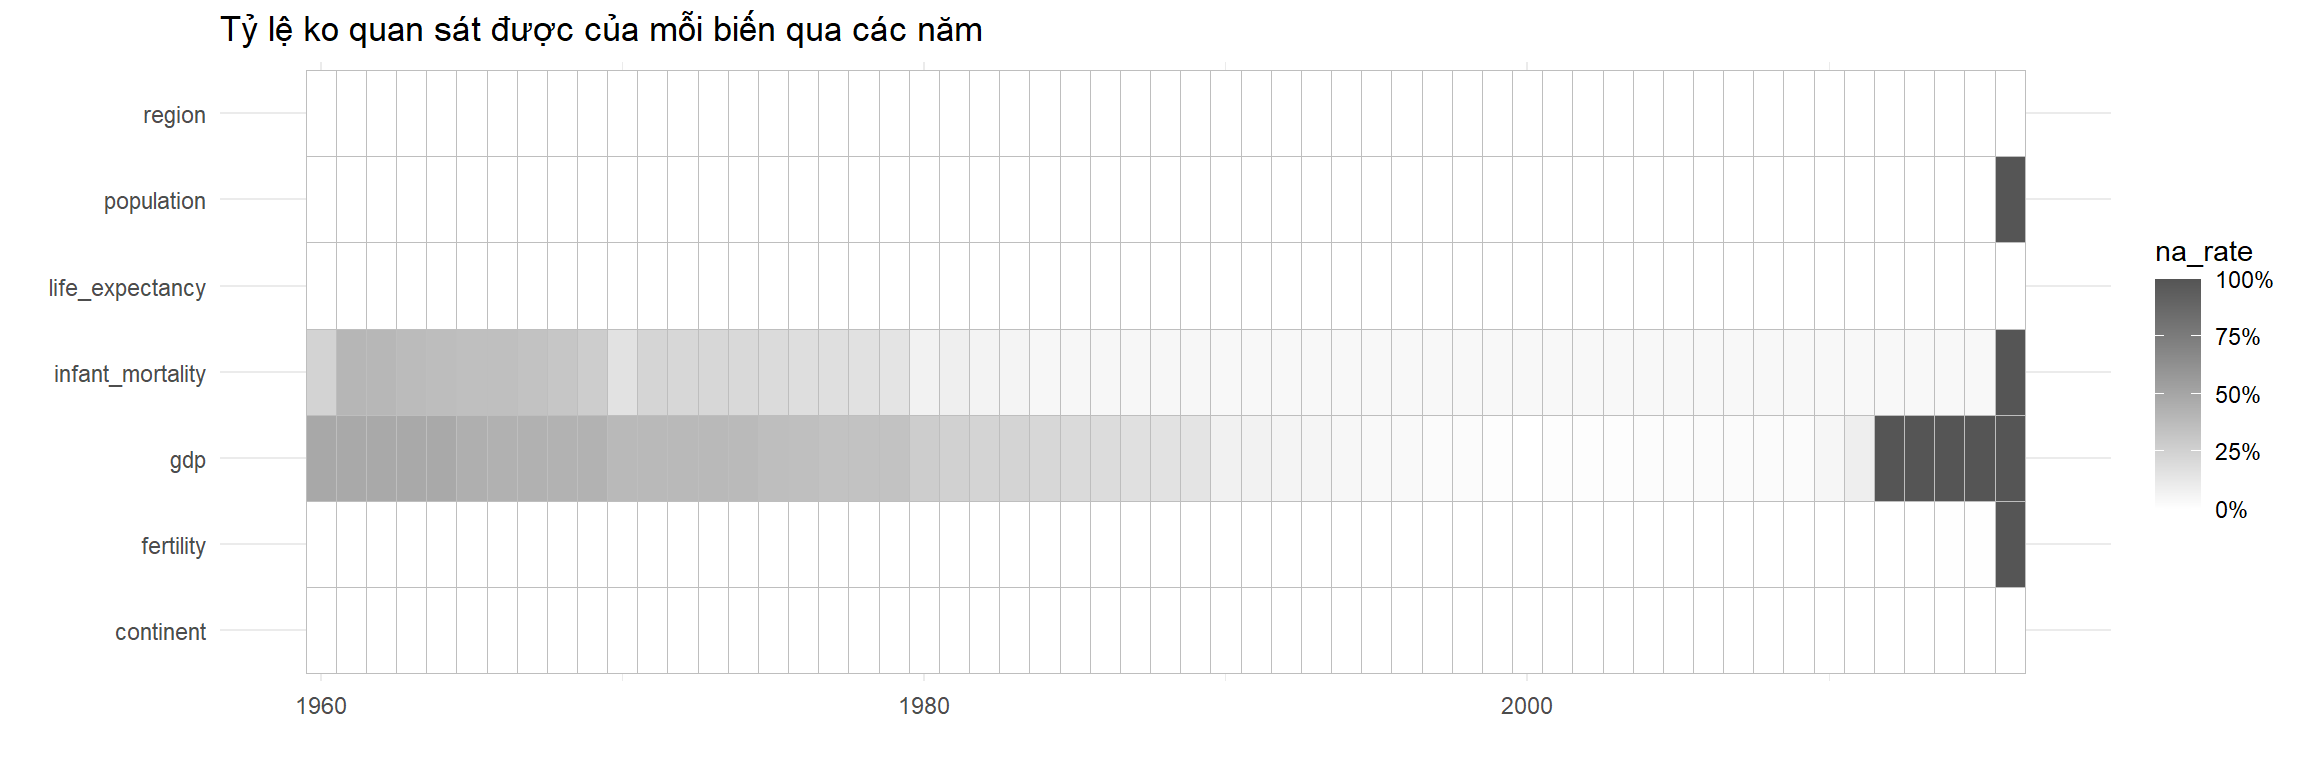
\includegraphics{02-literature_files/figure-latex/unnamed-chunk-5-1.pdf}

\begin{Shaded}
\begin{Highlighting}[]
\CommentTok{\# To view other plots, you can print them one by one:}
\CommentTok{\# print(plot\_list[["V1\_V2"]]) \# For example}

\FunctionTok{library}\NormalTok{(gridExtra)}
\end{Highlighting}
\end{Shaded}

\begin{verbatim}
## 
## Attaching package: 'gridExtra'
\end{verbatim}

\begin{verbatim}
## The following object is masked from 'package:dplyr':
## 
##     combine
\end{verbatim}

\begin{Shaded}
\begin{Highlighting}[]
\CommentTok{\# Assuming \textquotesingle{}plot\_list\textquotesingle{} contains all 15 ggplot objects from the previous example}
\CommentTok{\# Arrange plots in a 3x5 grid}
\NormalTok{grid\_layout }\OtherTok{\textless{}{-}} \FunctionTok{do.call}\NormalTok{(grid.arrange, }\FunctionTok{c}\NormalTok{(plot\_list, }\AttributeTok{ncol=}\DecValTok{5}\NormalTok{, }\AttributeTok{nrow=}\DecValTok{3}\NormalTok{))}
\end{Highlighting}
\end{Shaded}

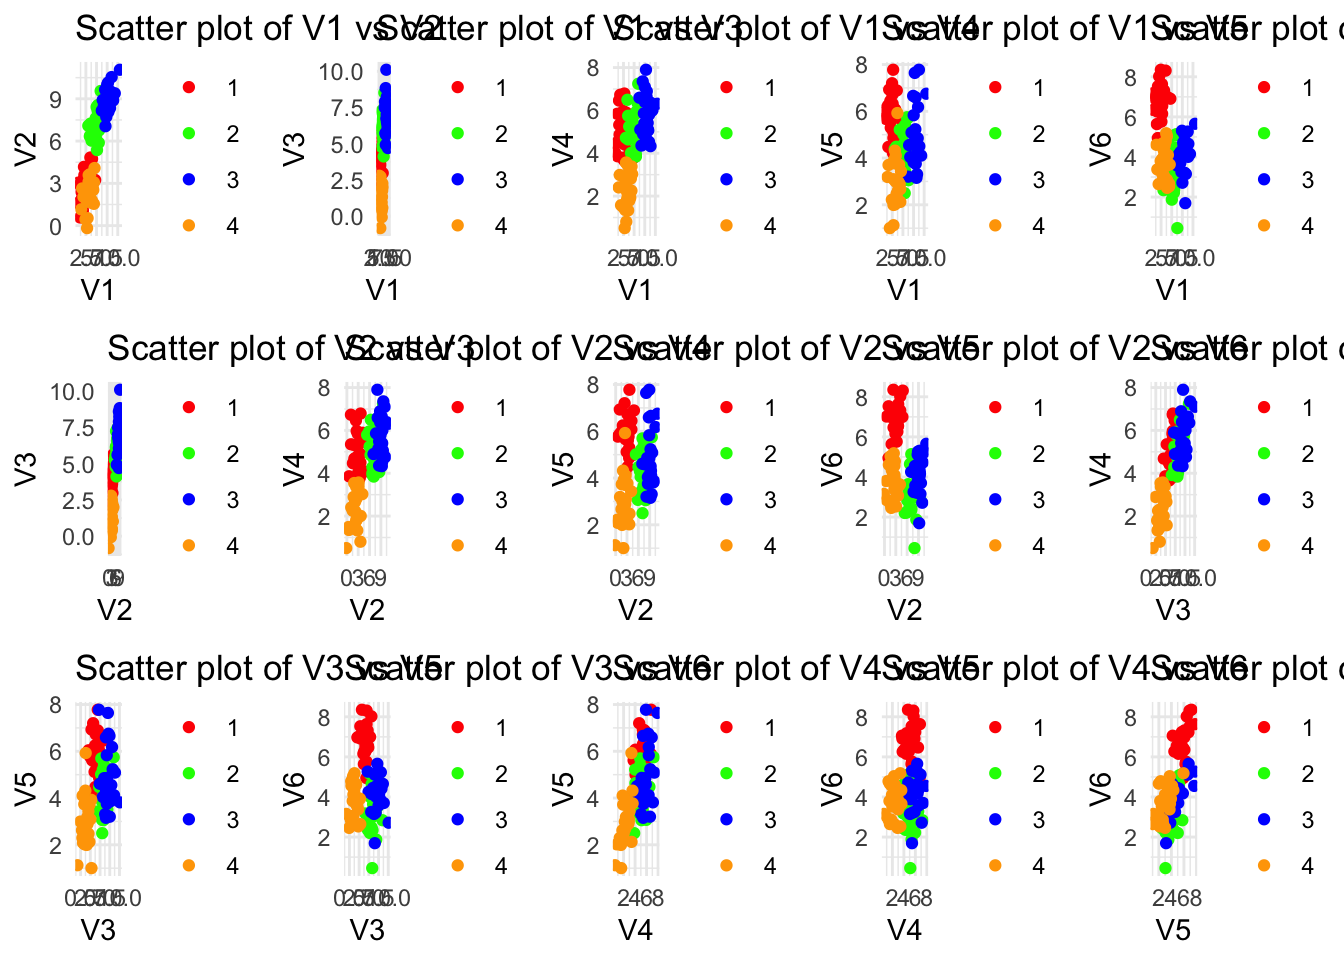
\includegraphics{02-literature_files/figure-latex/unnamed-chunk-5-2.pdf}

Rất nhiều bài toán ứng dụng thực tế rơi vào bối cảnh của thuật toán học có giám sát hoặc không giám sát. Tuy nhiên, có một vài trường hợp bài toán có thể không được phân loại rõ ràng vào loại học có giám sát hay không giám sát. Đơn giản như ta có một tập dữ liệu với \emph{n} quan sát, với \emph{m (m \textless{} n)} quan sát đầu tiên, chúng ta có cả biến mục tiêu (response) và biến dự báo (predictors), nhưng với \emph{n - m} quan sát còn lại, chúng ta chỉ có các biến dự báo (predictors) mà không còn biến mục tiêu (response) nữa. Những dữ liệu như vậy có thể xuất hiện trong trường hợp chi phí để thu thập dữ liệu cho các biến dự báo khá rẻ, trong khi đó các biến mục tiêu để thu thập thì cần tốn kém hơn rất nhiều. Chúng ta có thể gọi trường hợp này là bài toán học bán giám sát (semi-supervised learning problem). Đối với trường hợp này, chúng ta sẽ cần một phương pháp xử lý dữ liệu thống kê hiệu quả cho cả \emph{m} quan sát có biến mục tiêu và \emph{n - m} quan sát không có biến mục tiêu, tuy nhiên trong quyển sách này chúng tôi sẽ không giới thiệu các phương pháp đó.

\hypertarget{buxe0i-touxe1n-hux1ed3i-quy-vuxe0-buxe0i-touxe1n-phuxe2n-loux1ea1i}{%
\subsubsection{Bài toán hồi quy và bài toán phân loại}\label{buxe0i-touxe1n-hux1ed3i-quy-vuxe0-buxe0i-touxe1n-phuxe2n-loux1ea1i}}

Các biến thường được chia ra làm hai loại rõ ràng là biến định lượng và biến định tính. Biến định lượng có thể liệt kê ra một vài ví dụ tiêu biểu như tuổi, thu nhập, số lượng nhà đang sở hữu\ldots. Trong khi đó, biến định tính là các biến nhận một giá trị trong K loại khác nhau, ví dụ như tình trạng hôn nhân (Đã kết hôn/Chưa kết hôn), tình hình tín dụng (Đã vỡ nợ/Chưa vỡ nợ), tình hình bệnh tiểu đường (Không bị/Tuýp 1/Tuýp 2/Tuýp 3). Chúng ta thường phân các bài toán mà biến mục tiêu (response) thuộc loại biến định lượng là bài toán hồi quy, trong khi biến mục tiêu thuộc loại biến định tính thì gọi là bài toán phân loại. Dù trong nhiều trường hợp việc phân loại này hoạt động rất tốt, rất rõ ràng, nhưng đôi khi cũng tồn tại vài trường hợp mà các bài toán không được phân loại thực sự rõ ràng vào hai loại này. Các bài toán không được phân loại hẳn vào một loại ta có thể lấy một vài ví dụ như bài toán hồi quy logistic (chương 4) với biến mục tiêu là biến định tính, vốn luôn được coi là thuộc lớp bài toán phân loại, nhưng vì bản chất chúng tính toán xác suất mà biến mục tiêu rơi vào loại k (ví dụ như xác suất người bị tiểu đường bị tiểu đường Tuýp 2), nên chúng cũng có thể coi là bài toán hồi quy. Hay như các phương pháp như K - mean neighboring (KNN) hoặc Boosting đều cũng đều có thể sử dụng cho cả bài toán phân loại và bài toán hồi quy.

Thông thường, chúng ta sẽ dựa vào các biến mục tiêu là biến định tính hay biến định lượng để xác định bài toán của chúng ta là bài toán phân loại hay bài toán hồi quy, còn những biến dự báo (predictors) thuộc loại gì thì thường không ảnh hưởng đến cách chúng ta phân loại bài toán. Thực tế, hầu hết những phương pháp thống kê trong quyển sách này đều sử dụng được bất kể biến dụ báo là biến định lượng hay biến định tính, nếu là biến định tính chúng ta thường có phương pháp mã hoá biến trước khi thực hiện xây dựng mô hình thống kê.

\hypertarget{ux111uxe1nh-giuxe1-sux1ef1-chuxednh-xuxe1c-cux1ee7a-muxf4-huxecnh}{%
\subsection{Đánh giá sự chính xác của mô hình}\label{ux111uxe1nh-giuxe1-sux1ef1-chuxednh-xuxe1c-cux1ee7a-muxf4-huxecnh}}

Mục đích chính của quyển sách này là đưa người đọc đi sâu hơn vào thế giới của thống kê, nơi mà những phương pháp đã được xây dựng vượt xa hoàn toàn phương pháp hồi quy tuyến tính truyền thống. Tại sao chúng ta cần phải học nhiều phương pháp thống kê thay vì chỉ học một phương pháp thống kê tốt nhất? Bởi vì không bao giờ có gì là miễn phí hoàn toàn (free lunch) trong thống kê, có nghĩa là không có một mô hình nào vượt trội hoàn toàn so với các mô hình khác trong mọi loại dữ liệu. Trong một bộ dữ liệu, có một phương pháp thống kê nào đó cho ra kết quả tốt nhất, nhưng cũng có thể sẽ có một phương pháp thống kê khác cho ra kết quả tốt hơn trên một bộ dữ liệu khác gần như tương tự. Vậy nên, một trong những công việc quan trọng của các nhà thống kê đó là chọn lựa phương pháp thống kê tốt nhất khi gặp phải một bộ dữ liệu bất kỳ, đây là một trong những công việc khó và phức tạp nhất trong thực tế. Trong phần này, chúng tôi sẽ thảo luân về một vài khái niệm sẽ xuất hiện khi chúng ta lựa chọn một mô hình thống kê nào đó phù hợp với dữ liệu của chúng ta, và chúng tôi cũng sẽ lồng ghép các khái niệm được thể hiện ở đây vào các bài toán thực tế trong phần sau của quyển sách này.

\hypertarget{ux111o-ux111ux1ed9-khux1edbp-cux1ee7a-muxf4-huxecnh}{%
\subsubsection{Đo độ khớp của mô hình}\label{ux111o-ux111ux1ed9-khux1edbp-cux1ee7a-muxf4-huxecnh}}

Để đánh giá hiệu quả của một phương pháp thống kê trên một tập dữ liệu nhất định, chúng ta cần phải theo dõi xem các dự đoán của mô hình khớp với các giá trị dữ liệu quan sát được đến đâu. Từ đó, người ta đã nghĩ ra các phương pháp để lượng hoá sự gần sát của các dự đoán và các giá trị dữ liệu quan sát thực tế. Trong các bài toán hồi quy, giá trị đo thường được người ta sử dụng nhất là trung bình bình phương sai số (MSE), được cho bởi công thức

\begin{align}
MSE = \dfrac{1}{n} \sum\limits_{i = 1}^{n} \left[y_i - \hat{f}(x_i)\right]^2
\label{eq:mse}
\end{align}

trong đó \(\hat{f}(x_i)\) là dự đoán của hàm \hat{f} đối với quan sát thứ i. Giá trị trung bình bình phương sai số (MSE) sẽ càng trở nên nhỏ nếu như giá trị dự đoán càng gần với giá trị dữ liệu quan sát thực tế, và càng lớn nếu như có một vài quan sát có kết quả dự đoán cách xa so với giá. trị dữ liệu quan sát thực tế. Phương trình \eqref{eq:mse} được tính dựa trên tập dữ liệu huấn luyện mà được sử dụng để tạo ra hàm \hat{f} khớp với mô hình. Vậy nên nó thường được gọi bằng cái tên chính xác hơn là trung bình bình phương sai số của tập dữ liệu huấn luyện (training MSE). Dù vậy, trong thực tế, chúng ta không quá quan tâm đến sự chính xác của mô hình trên dữ liệu huấn luyện mà câu hỏi quan trọng hơn là: \emph{Sự chính xác của mô hình khi chúng ta áp dụng nó vào các quan sát trong tập dữ liệu kiểm thử liệu có còn tốt hay không?}
Chúng ta quan tâm đến các số liệu này bởi vì những người xây dựng mô hình để dự báo luôn muốn xây dựng một mô hình có khả năng dự đoán tương lai tốt nhất. Ta lấy ví dụ những chuyên gia muốn xây dựng một mô hình để dự đoán giá cổ phiếu trong tương lai, dựa vào dữ liệu giá cổ phiếu trong 6 tháng trước. Khi đó, sẽ không có nhiều ý nghĩa nếu mô hình cho ra kết quả dự đoán dữ liệu giá cổ phiếu 2 tuần trước gần với giá trị đã được ghi nhận, bởi vì đó là thông tin chúng ta và cả mô hình đều được biết rồi, mà quan trọng là mô hình đó phải dự báo được khá chính xác giá cổ phiếu trong tương lai (thông tin chưa ai biết) để các nhà đầu tư có thể đưa ra chiến lược phù hợp. Tương tự, đối với bài toán dự đoán khả năng bị tiểu đường của các bệnh nhân, chúng ta cũng thường chỉ quan tâm đến khả năng mô hình được xây dựng dự báo chính xác những bệnh nhân trong tương lai, chứ không phải là dự đoán xem những bệnh nhân trước đó bị tiểu đường loại nào. Thực tế, ta không hề có dữ liệu về những quan sát ở trong tương lai, nên để kiểm tra mô hình ta thường chia dữ liệu của chúng ta thành ít nhất hai tập dữ liệu huấn luyện và tập dữ liệu kiểm thử. Bởi vì khi tập dữ liệu kiểm thử không được đưa vào để huấn luyện mô hình, có nghĩa là những dữ liệu đó sẽ được coi như là dữ liệu mới chưa bao giờ gặp trong mô hình, nên nếu như mô hình có thể dự đoán với độ chính xác cao những quan sát trong tập dữ liệu kiểm thử thì người ta kỳ vọng rằng nó cũng sẽ chạy tốt khi áp dụng với những quan sát trong tương lai.

Để diễn tả một cách toán học, giả sử chúng ta đang muốn khớp một phương pháp thống kê nào đó dựa trên tập dữ liệu huấn luyện \({(x_1, y_1), (x_2, y_2),...,(x_n, y_n)}\), kết quả chúng ta sẽ thu được một hàm \(\hat{f}\). Từ đó chúng ta có thể tính các giá trị \(\hat{f}(x_1), \hat{f}(x_2),..., \hat{f}(x_n)\). Nếu những giá trị đó mà gần với các giá trị \(y_1, y_2,...,y_n\) thì trung bình bình phương sai số của tập dữ liệu huấn luyện (training MSE) được cho bởi công thức \eqref{eq:mse} sẽ rất nhỏ. Nhưng chúng ta lại quan tâm hơn đến liệu giá trị \(\hat{f}(x_0)\) có xấp xỉ bằng \(y_0\) hay không, với \((x_0, y_0)\) là một quan sát thuộc tập dữ liệu kiểm thử, chưa được đưa vào để tạo ra hàm \(\hat{f}\). Các chuyên gia thường muốn lựa chọn được mô hình có trung bình bình phương sai số trên tập dữ liệu kiểm thử (test MSE) nhỏ nhất. Nói cách khác, nếu chúng ta có một lượng lớn các dữ liệu trong tập dữ liệu kiểm thử, chúng ta có thể tính

\begin{align}
Average\left[y_0 - \hat{f}(x_0)\right]^2 
\end{align}

giá trị trung bình bình phương sai số trên tập dữ liệu kiểm thử với các quan sát \((x_0, y_0)\), và chúng ta thường lựa chọn mô hình sao cho giá trị này càng nhỏ càng tốt.

\hypertarget{sux1ef1-ux111uxe1nh-ux111ux1ed5i-giux1eefa-ux111ux1ed9-chux1ec7ch-vuxe0-phux1b0ux1a1ng-sai}{%
\subsection{Sự đánh đổi giữa độ chệch và phương sai}\label{sux1ef1-ux111uxe1nh-ux111ux1ed5i-giux1eefa-ux111ux1ed9-chux1ec7ch-vuxe0-phux1b0ux1a1ng-sai}}

Dáng đường cong chữ U (U-shape) của đường sai số bình phương trung bình trên tập dữ liệu kiểm thử thể hiện hai tính chất rất quan trọng của một phươung pháp học thống kê hiện đại. Cần phải nhắc lại rằng trong quyển sách này chúng tôi sẽ không đưa ra những chứng minh toán học quá phức tạp, nhưng để thể hiện tính chất đánh đổi giữa độ chệch và phương sai này, chúng ta vẫn có thể đi từ một công thức đơn giản liên quan đến giá trị kỳ vọng của sai số bình phương trung bình của một giá trị \(x_0\). Chúng ta có thể tách giá trị kỳ đó ra thành ba phần chính: phương sai của \(\hat{f}(x_0)\), độ chệch bình phương của \(\hat{f}(x_0)\), và phương sai của sai số \(\epsilon\) như sau:

\begin{equation}
E\left(y_0 - \hat{f}(x_0)\right)^2 = Var\left(\hat{f}(x_0)\right) + \left[Bias(\hat{f}(x_0))\right]^2 + Var(\epsilon)
\label{eq:bias_variance}
\end{equation}

Trong đó, \(E\left(y_0 - \hat{f}(x_0)\right)^2\) được định nghĩa là giá trị kỳ vọng của trung bình bình phương sai số trên tập dữ liệu kiểm thử với quan sát \(x_0\). Nếu chúng ta lặp đi lặp lại quá trình ước lượng các hàm f này với một lượng lớn tập dữ liệu huấn luyện, và test mỗi mô hình với quan sát \(x_0\). Giá trị kỳ vọng tổng thể của trung bình bình phương sai số (overall expected test MSE) có thể được tính bằng cách lấy trung bình của \(E\left(y_0 - \hat{f}(x_0)\right)^2\) với tất cả các quan sát \(x_0\) trong tập dữ liệu kiểm thử.

Phương trình \ref{eq:bias_variance} cho chúng ta biết rằng nếu muốn giảm giá trị sai số kỳ vọng trên tập dữ liệu kiểm thử, chúng ta cần chọn phương pháp học thống kê sao cho đồng thời đạt được cả hai mục tiêu là phương sai thấp và độ chệch thấp. Chúng ta cũng cần lưu ý rằng giá trị MSE kỳ vọng không bao giờ thấp hơn Var(\(\epsilon\)), đó là phần sai số không thể giảm trong công thức \ref{eq:re_irre_error}.

\hypertarget{phux1b0ux1a1ng-sai-cux1ee7a-muxf4-huxecnh}{%
\subsubsection{Phương sai của mô hình}\label{phux1b0ux1a1ng-sai-cux1ee7a-muxf4-huxecnh}}

Vậy thì rốt cuộc, chúng ta nên hiểu phương sai (variance) và độ chệch (bias) của phương pháp học thống kê như thế nào cho đúng? Phương sai (variance) nói đến lượng thay đổi của hàm \(\hat{f}\) khi chúng ta ước lượng hàm \(\hat{f}\) bằng một dữ liệu huấn luyện khác. Bởi vì dữ liệu huấn luyện được sử dụng để ước lượng hàm \(\hat{f}\), nên việc chúng ta sử dụng dữ liệu huấn luyện khác nhau sẽ cho ra hàm \(\hat{f}\) khác nhau. Tuy nhiên, trong trường hợp lý tưởng, ước lượng cho hàm f không nên chênh lệch quá nhiều giữa các dữ liệu huấn luyện khác nhau. Nếu một phương pháp học thống kê nào đó có sự thay đổi lớn về hàm \(\hat{f}\) dù chúng ta chỉ thay đổi dữ liệu đầu vào một chút, có nghĩa là phương pháp học thống kê đó có phương sai cao (high variance). Nhìn chung, các phương pháp học thống kê càng linh hoạt (ví dụ như neural networks, decision tree, random forests) thường có phương sai càng cao.

\textbf{Ở đây tiếp tục simulate ra một dữ liệu nữa để thể hiện phương sai cao của phương pháp more flexible}

\begin{Shaded}
\begin{Highlighting}[]
\CommentTok{\# Define the number of variables}
\NormalTok{number\_of\_variables }\OtherTok{\textless{}{-}} \DecValTok{1}\SpecialCharTok{:}\DecValTok{15}

\CommentTok{\# Train MSE decreases exponentially from 7 to below 0.3}
\NormalTok{train\_mse }\OtherTok{\textless{}{-}} \DecValTok{7} \SpecialCharTok{*} \FunctionTok{exp}\NormalTok{(}\SpecialCharTok{{-}}\FloatTok{0.5} \SpecialCharTok{*}\NormalTok{ number\_of\_variables)}
\CommentTok{\# Manually set the last value to ensure it\textquotesingle{}s just below 0.3}
\NormalTok{train\_mse[}\FunctionTok{length}\NormalTok{(train\_mse)] }\OtherTok{\textless{}{-}} \FloatTok{0.3}

\CommentTok{\# Test MSE: starts at 7.5, decreases to a point, then increases again}
\NormalTok{test\_mse }\OtherTok{\textless{}{-}} \FunctionTok{numeric}\NormalTok{(}\FunctionTok{length}\NormalTok{(number\_of\_variables))}
\NormalTok{test\_mse[}\DecValTok{1}\NormalTok{] }\OtherTok{\textless{}{-}} \FloatTok{7.5} \CommentTok{\# Starting point for Test MSE}

\CommentTok{\# Calculate Test MSE values}
\ControlFlowTok{for}\NormalTok{ (i }\ControlFlowTok{in} \DecValTok{2}\SpecialCharTok{:}\FunctionTok{length}\NormalTok{(test\_mse)) \{}
  \ControlFlowTok{if}\NormalTok{ (i }\SpecialCharTok{\textless{}=} \DecValTok{4}\NormalTok{) \{}
    \CommentTok{\# Decreasing phase for the first 4 variables}
\NormalTok{    test\_mse[i] }\OtherTok{\textless{}{-}}\NormalTok{ test\_mse[i}\DecValTok{{-}1}\NormalTok{] }\SpecialCharTok{{-}} \FloatTok{0.5}
\NormalTok{  \} }\ControlFlowTok{else}\NormalTok{ \{}
    \CommentTok{\# Increasing phase after the 4th variable}
\NormalTok{    test\_mse[i] }\OtherTok{\textless{}{-}} \DecValTok{6} \SpecialCharTok{+} \FloatTok{0.1} \SpecialCharTok{*}\NormalTok{ (i }\SpecialCharTok{{-}} \DecValTok{4}\NormalTok{)}\SpecialCharTok{\^{}}\DecValTok{2}
\NormalTok{  \}}
\NormalTok{\}}

\CommentTok{\# Ensure Test MSE is always at least 2 units greater than Train MSE}
\NormalTok{test\_mse }\OtherTok{\textless{}{-}} \FunctionTok{pmax}\NormalTok{(test\_mse, train\_mse }\SpecialCharTok{+} \DecValTok{2}\NormalTok{)}

\CommentTok{\# Plotting}
\FunctionTok{plot}\NormalTok{(number\_of\_variables, train\_mse, }\AttributeTok{type=}\StringTok{\textquotesingle{}l\textquotesingle{}}\NormalTok{, }\AttributeTok{pch=}\DecValTok{19}\NormalTok{, }\AttributeTok{col=}\StringTok{\textquotesingle{}blue\textquotesingle{}}\NormalTok{, }\AttributeTok{ylim=}\FunctionTok{c}\NormalTok{(}\DecValTok{0}\NormalTok{, }\FunctionTok{max}\NormalTok{(test\_mse)), }\AttributeTok{xlim =} \FunctionTok{c}\NormalTok{(}\DecValTok{1}\NormalTok{,}\DecValTok{14}\NormalTok{), }\AttributeTok{ylab=}\StringTok{\textquotesingle{}MSE\textquotesingle{}}\NormalTok{, }\AttributeTok{xlab=}\StringTok{\textquotesingle{}Number of Variables\textquotesingle{}}\NormalTok{, }\AttributeTok{main=}\StringTok{\textquotesingle{}Train vs Test MSE\textquotesingle{}}\NormalTok{)}
\FunctionTok{lines}\NormalTok{(number\_of\_variables, test\_mse, }\AttributeTok{type=}\StringTok{\textquotesingle{}l\textquotesingle{}}\NormalTok{, }\AttributeTok{pch=}\DecValTok{19}\NormalTok{, }\AttributeTok{col=}\StringTok{\textquotesingle{}red\textquotesingle{}}\NormalTok{, }\AttributeTok{lty=}\DecValTok{2}\NormalTok{)}
\CommentTok{\#points(number\_of\_variables, test\_mse, pch=19, col=\textquotesingle{}red\textquotesingle{}) \# Adding points for test MSE}

\FunctionTok{legend}\NormalTok{(}\StringTok{"topright"}\NormalTok{, }\AttributeTok{legend=}\FunctionTok{c}\NormalTok{(}\StringTok{"Train MSE"}\NormalTok{, }\StringTok{"Test MSE"}\NormalTok{), }\AttributeTok{col=}\FunctionTok{c}\NormalTok{(}\StringTok{"blue"}\NormalTok{, }\StringTok{"red"}\NormalTok{), }\AttributeTok{pch=}\DecValTok{19}\NormalTok{, }\AttributeTok{lty=}\DecValTok{1}\SpecialCharTok{:}\DecValTok{2}\NormalTok{)}
\end{Highlighting}
\end{Shaded}

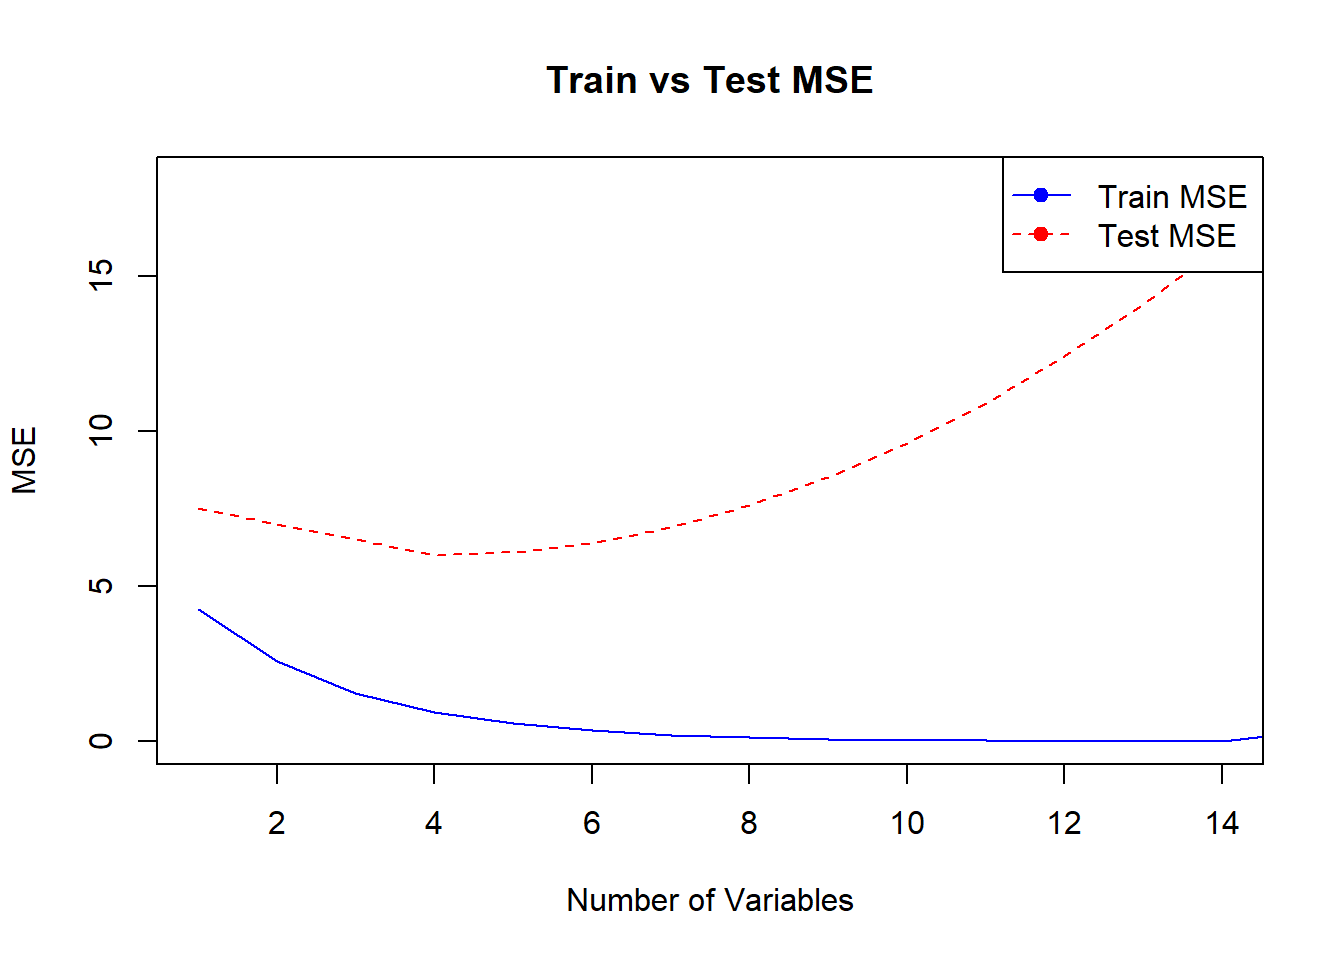
\includegraphics{02-literature_files/figure-latex/unnamed-chunk-6-1.pdf}

\begin{Shaded}
\begin{Highlighting}[]
\CommentTok{\# Required libraries}
\FunctionTok{library}\NormalTok{(caret)}
\end{Highlighting}
\end{Shaded}

\begin{verbatim}
## Loading required package: lattice
\end{verbatim}

\begin{Shaded}
\begin{Highlighting}[]
\FunctionTok{set.seed}\NormalTok{(}\DecValTok{42}\NormalTok{)}

\CommentTok{\# Simulating data with 15 independent variables}
\NormalTok{n }\OtherTok{\textless{}{-}} \DecValTok{200} \CommentTok{\# Number of observations}
\NormalTok{p }\OtherTok{\textless{}{-}} \DecValTok{15} \CommentTok{\# Number of variables}

\CommentTok{\# Simulate relevant variables with stronger signal}
\NormalTok{num\_relevant }\OtherTok{\textless{}{-}} \DecValTok{5}
\NormalTok{X\_relevant }\OtherTok{\textless{}{-}} \FunctionTok{matrix}\NormalTok{(}\FunctionTok{rnorm}\NormalTok{(n }\SpecialCharTok{*}\NormalTok{ num\_relevant), }\AttributeTok{ncol =}\NormalTok{ num\_relevant)}
\NormalTok{beta\_relevant }\OtherTok{\textless{}{-}} \FunctionTok{runif}\NormalTok{(num\_relevant, }\SpecialCharTok{{-}}\DecValTok{2}\NormalTok{, }\DecValTok{2}\NormalTok{) }\CommentTok{\# Random coefficients for relevant variables}

\CommentTok{\# Simulate irrelevant variables with weaker signal (noise)}
\NormalTok{num\_irrelevant }\OtherTok{\textless{}{-}}\NormalTok{ p }\SpecialCharTok{{-}}\NormalTok{ num\_relevant}
\NormalTok{X\_irrelevant }\OtherTok{\textless{}{-}} \FunctionTok{matrix}\NormalTok{(}\FunctionTok{rnorm}\NormalTok{(n }\SpecialCharTok{*}\NormalTok{ num\_irrelevant), }\AttributeTok{ncol =}\NormalTok{ num\_irrelevant)}
\NormalTok{beta\_irrelevant }\OtherTok{\textless{}{-}} \FunctionTok{runif}\NormalTok{(num\_irrelevant, }\SpecialCharTok{{-}}\FloatTok{0.1}\NormalTok{, }\FloatTok{0.1}\NormalTok{) }\CommentTok{\# Random coefficients for irrelevant variables}

\CommentTok{\# Combine relevant and irrelevant variables}
\NormalTok{X }\OtherTok{\textless{}{-}} \FunctionTok{cbind}\NormalTok{(X\_relevant, X\_irrelevant)}
\NormalTok{beta }\OtherTok{\textless{}{-}} \FunctionTok{c}\NormalTok{(beta\_relevant, beta\_irrelevant)}

\CommentTok{\# Noise}
\NormalTok{epsilon }\OtherTok{\textless{}{-}} \FunctionTok{rnorm}\NormalTok{(n)}

\CommentTok{\# Response variable}
\NormalTok{Y }\OtherTok{\textless{}{-}}\NormalTok{ X }\SpecialCharTok{\%*\%}\NormalTok{ beta }\SpecialCharTok{+}\NormalTok{ epsilon}

\CommentTok{\# Splitting the data into training and testing sets}
\FunctionTok{set.seed}\NormalTok{(}\DecValTok{42}\NormalTok{)}
\NormalTok{trainIndex }\OtherTok{\textless{}{-}} \FunctionTok{createDataPartition}\NormalTok{(Y, }\AttributeTok{p =}\NormalTok{ .}\DecValTok{8}\NormalTok{, }\AttributeTok{list =} \ConstantTok{FALSE}\NormalTok{)}
\NormalTok{X\_train }\OtherTok{\textless{}{-}}\NormalTok{ X[trainIndex, ]}
\NormalTok{Y\_train }\OtherTok{\textless{}{-}}\NormalTok{ Y[trainIndex]}
\NormalTok{X\_test }\OtherTok{\textless{}{-}}\NormalTok{ X[}\SpecialCharTok{{-}}\NormalTok{trainIndex, ]}
\NormalTok{Y\_test }\OtherTok{\textless{}{-}}\NormalTok{ Y[}\SpecialCharTok{{-}}\NormalTok{trainIndex]}

\CommentTok{\# Initialize vectors to store metrics}
\NormalTok{train\_mse }\OtherTok{\textless{}{-}} \FunctionTok{numeric}\NormalTok{(p)}
\NormalTok{test\_mse }\OtherTok{\textless{}{-}} \FunctionTok{numeric}\NormalTok{(p)}

\CommentTok{\# Fit models and calculate MSE for training and testing sets}
\ControlFlowTok{for}\NormalTok{ (i }\ControlFlowTok{in} \DecValTok{1}\SpecialCharTok{:}\NormalTok{p) \{}
\NormalTok{  model }\OtherTok{\textless{}{-}} \FunctionTok{lm}\NormalTok{(Y\_train }\SpecialCharTok{\textasciitilde{}}\NormalTok{ X\_train[, }\DecValTok{1}\SpecialCharTok{:}\NormalTok{i])}
\NormalTok{  train\_predictions }\OtherTok{\textless{}{-}} \FunctionTok{predict}\NormalTok{(model, }\FunctionTok{data.frame}\NormalTok{(X\_train[, }\DecValTok{1}\SpecialCharTok{:}\NormalTok{i]))}
\NormalTok{  test\_predictions }\OtherTok{\textless{}{-}} \FunctionTok{predict}\NormalTok{(model, }\FunctionTok{data.frame}\NormalTok{(X\_test[, }\DecValTok{1}\SpecialCharTok{:}\NormalTok{i]))}
  
  \CommentTok{\# Calculating MSE}
\NormalTok{  train\_mse[i] }\OtherTok{\textless{}{-}} \FunctionTok{mean}\NormalTok{((Y\_train }\SpecialCharTok{{-}}\NormalTok{ train\_predictions)}\SpecialCharTok{\^{}}\DecValTok{2}\NormalTok{)}
\NormalTok{  test\_mse[i] }\OtherTok{\textless{}{-}} \FunctionTok{mean}\NormalTok{((Y\_test }\SpecialCharTok{{-}}\NormalTok{ test\_predictions)}\SpecialCharTok{\^{}}\DecValTok{2}\NormalTok{)}
\NormalTok{\}}
\end{Highlighting}
\end{Shaded}

\begin{verbatim}
## Warning: 'newdata' had 40 rows but variables found have 160 rows

## Warning: 'newdata' had 40 rows but variables found have 160 rows

## Warning: 'newdata' had 40 rows but variables found have 160 rows

## Warning: 'newdata' had 40 rows but variables found have 160 rows

## Warning: 'newdata' had 40 rows but variables found have 160 rows

## Warning: 'newdata' had 40 rows but variables found have 160 rows

## Warning: 'newdata' had 40 rows but variables found have 160 rows

## Warning: 'newdata' had 40 rows but variables found have 160 rows

## Warning: 'newdata' had 40 rows but variables found have 160 rows

## Warning: 'newdata' had 40 rows but variables found have 160 rows

## Warning: 'newdata' had 40 rows but variables found have 160 rows

## Warning: 'newdata' had 40 rows but variables found have 160 rows

## Warning: 'newdata' had 40 rows but variables found have 160 rows

## Warning: 'newdata' had 40 rows but variables found have 160 rows

## Warning: 'newdata' had 40 rows but variables found have 160 rows
\end{verbatim}

\begin{Shaded}
\begin{Highlighting}[]
\CommentTok{\# Plotting}
\FunctionTok{plot}\NormalTok{(}\DecValTok{1}\SpecialCharTok{:}\NormalTok{p, train\_mse, }\AttributeTok{type =} \StringTok{"b"}\NormalTok{, }\AttributeTok{pch =} \DecValTok{19}\NormalTok{, }\AttributeTok{col =} \StringTok{"blue"}\NormalTok{, }\AttributeTok{xlab =} \StringTok{"Number of Variables"}\NormalTok{, }\AttributeTok{ylab =} \StringTok{"MSE"}\NormalTok{, }\AttributeTok{ylim =} \FunctionTok{c}\NormalTok{(}\FunctionTok{min}\NormalTok{(}\FunctionTok{c}\NormalTok{(train\_mse, test\_mse)), }\FunctionTok{max}\NormalTok{(}\FunctionTok{c}\NormalTok{(train\_mse, test\_mse))), }\AttributeTok{main =} \StringTok{"MSE, Bias, and Variance vs Model Complexity"}\NormalTok{)}
\FunctionTok{points}\NormalTok{(}\DecValTok{1}\SpecialCharTok{:}\NormalTok{p, test\_mse, }\AttributeTok{type =} \StringTok{"b"}\NormalTok{, }\AttributeTok{pch =} \DecValTok{23}\NormalTok{, }\AttributeTok{col =} \StringTok{"red"}\NormalTok{, }\AttributeTok{bg =} \StringTok{"red"}\NormalTok{)}
\FunctionTok{legend}\NormalTok{(}\StringTok{"topright"}\NormalTok{, }\AttributeTok{legend =} \FunctionTok{c}\NormalTok{(}\StringTok{"Train MSE"}\NormalTok{, }\StringTok{"Test MSE"}\NormalTok{), }\AttributeTok{col =} \FunctionTok{c}\NormalTok{(}\StringTok{"blue"}\NormalTok{, }\StringTok{"red"}\NormalTok{), }\AttributeTok{pch =} \FunctionTok{c}\NormalTok{(}\DecValTok{19}\NormalTok{, }\DecValTok{23}\NormalTok{))}
\end{Highlighting}
\end{Shaded}

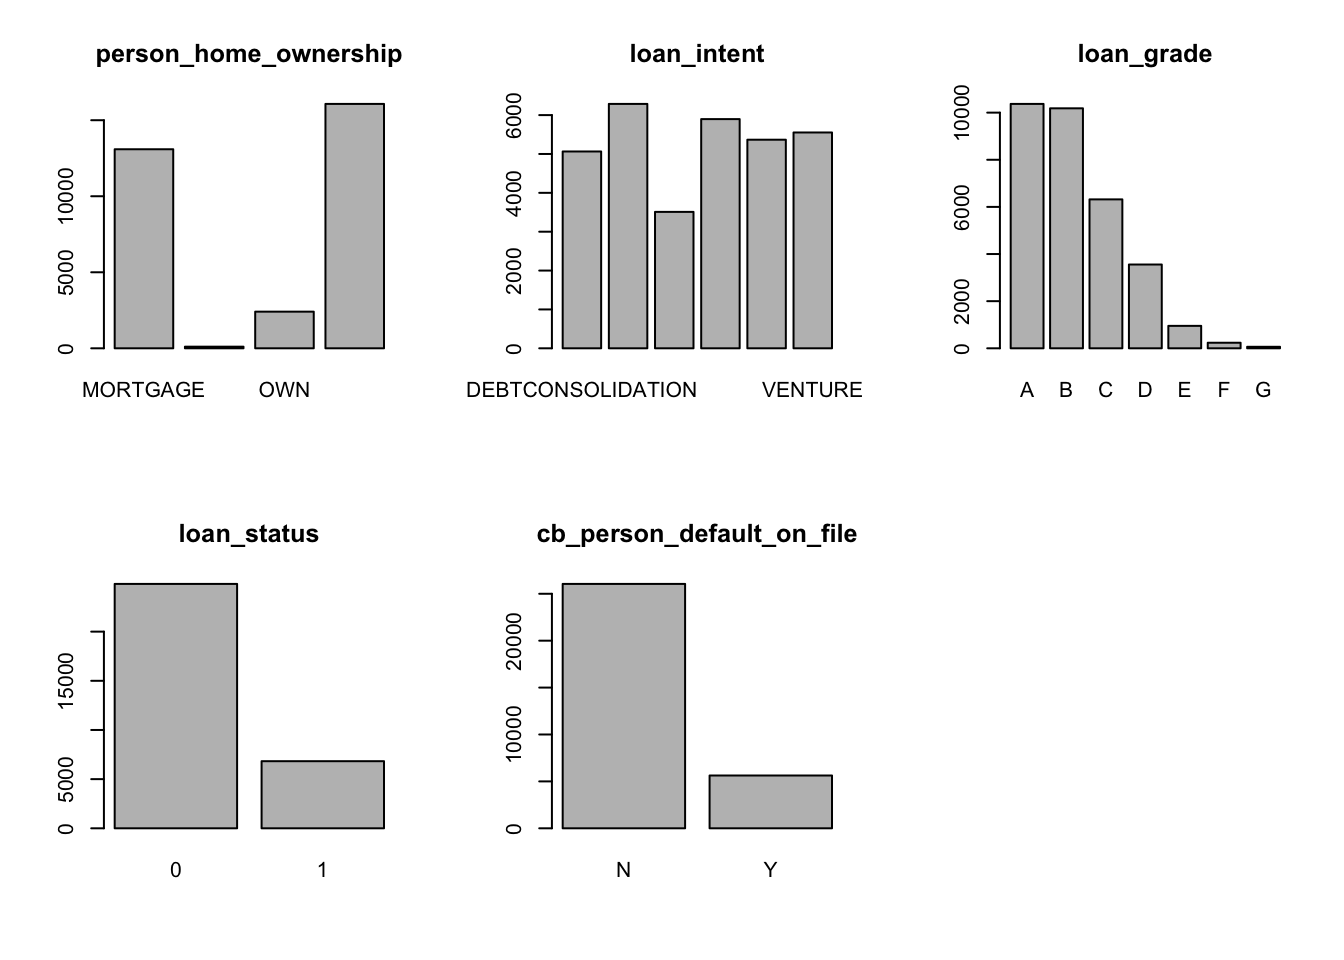
\includegraphics{02-literature_files/figure-latex/unnamed-chunk-7-1.pdf}

\begin{Shaded}
\begin{Highlighting}[]
\FunctionTok{set.seed}\NormalTok{(}\DecValTok{42}\NormalTok{)}
\FunctionTok{library}\NormalTok{(MASS) }\CommentTok{\# For true randomness in simulation}

\CommentTok{\# Simulating data}
\NormalTok{n }\OtherTok{\textless{}{-}} \DecValTok{1000} \CommentTok{\# Number of observations}
\NormalTok{p }\OtherTok{\textless{}{-}} \DecValTok{15} \CommentTok{\# Number of independent variables}
\NormalTok{X }\OtherTok{\textless{}{-}} \FunctionTok{matrix}\NormalTok{(}\FunctionTok{rnorm}\NormalTok{(n }\SpecialCharTok{*}\NormalTok{ p), }\AttributeTok{ncol =}\NormalTok{ p)}
\NormalTok{true\_beta }\OtherTok{\textless{}{-}} \FunctionTok{rnorm}\NormalTok{(p, }\AttributeTok{mean =} \FloatTok{0.2}\NormalTok{, }\AttributeTok{sd =} \FloatTok{0.5}\NormalTok{) }\CommentTok{\# True coefficients}
\NormalTok{Y }\OtherTok{\textless{}{-}}\NormalTok{ X }\SpecialCharTok{\%*\%}\NormalTok{ true\_beta }\SpecialCharTok{+} \FunctionTok{rnorm}\NormalTok{(n) }\CommentTok{\# Response with noise}

\CommentTok{\# Train{-}test split}
\NormalTok{train\_proportion }\OtherTok{\textless{}{-}} \FloatTok{0.5}
\NormalTok{train\_sample }\OtherTok{\textless{}{-}} \FunctionTok{sample}\NormalTok{(}\DecValTok{1}\SpecialCharTok{:}\NormalTok{n, }\AttributeTok{size =} \FunctionTok{floor}\NormalTok{(n }\SpecialCharTok{*}\NormalTok{ train\_proportion))}
\NormalTok{X\_train }\OtherTok{\textless{}{-}}\NormalTok{ X[train\_sample, ]}
\NormalTok{Y\_train }\OtherTok{\textless{}{-}}\NormalTok{ Y[train\_sample]}
\NormalTok{X\_test }\OtherTok{\textless{}{-}}\NormalTok{ X[}\SpecialCharTok{{-}}\NormalTok{train\_sample, ]}
\NormalTok{Y\_test }\OtherTok{\textless{}{-}}\NormalTok{ Y[}\SpecialCharTok{{-}}\NormalTok{train\_sample]}

\CommentTok{\# Calculate squared bias, variance, and MSE}
\NormalTok{calc\_metrics }\OtherTok{\textless{}{-}} \ControlFlowTok{function}\NormalTok{(i, X\_train, Y\_train, X\_test, Y\_test, true\_beta) \{}
  \CommentTok{\# Bootstrap predictions for variance estimation}
\NormalTok{  n\_bootstraps }\OtherTok{\textless{}{-}} \DecValTok{100}
\NormalTok{  n\_test }\OtherTok{\textless{}{-}} \FunctionTok{length}\NormalTok{(Y\_test)}
\NormalTok{  predictions\_test }\OtherTok{\textless{}{-}} \FunctionTok{matrix}\NormalTok{(}\AttributeTok{nrow =}\NormalTok{ n\_bootstraps, }\AttributeTok{ncol =}\NormalTok{ n\_test)}
  
  \ControlFlowTok{for}\NormalTok{ (b }\ControlFlowTok{in} \DecValTok{1}\SpecialCharTok{:}\NormalTok{n\_bootstraps) \{}
\NormalTok{    sample\_indices }\OtherTok{\textless{}{-}} \FunctionTok{sample}\NormalTok{(}\FunctionTok{nrow}\NormalTok{(X\_train), }\FunctionTok{nrow}\NormalTok{(X\_train), }\AttributeTok{replace =} \ConstantTok{TRUE}\NormalTok{)}
\NormalTok{    X\_train\_b }\OtherTok{\textless{}{-}}\NormalTok{ X\_train[sample\_indices, , drop }\OtherTok{=} \ConstantTok{FALSE}\NormalTok{]}
\NormalTok{    Y\_train\_b }\OtherTok{\textless{}{-}}\NormalTok{ Y\_train[sample\_indices]}
\NormalTok{    model\_b }\OtherTok{\textless{}{-}} \FunctionTok{lm}\NormalTok{(Y\_train\_b }\SpecialCharTok{\textasciitilde{}}\NormalTok{ X\_train\_b[, }\DecValTok{1}\SpecialCharTok{:}\NormalTok{i, }\AttributeTok{drop =} \ConstantTok{FALSE}\NormalTok{])}
    \CommentTok{\# Ensuring that newdata has the correct number of columns}
\NormalTok{    predictions\_test[b, ] }\OtherTok{\textless{}{-}} \FunctionTok{predict}\NormalTok{(model\_b, }\AttributeTok{newdata =} \FunctionTok{as.data.frame}\NormalTok{(X\_test[, }\DecValTok{1}\SpecialCharTok{:}\NormalTok{i, }\AttributeTok{drop =} \ConstantTok{FALSE}\NormalTok{]))}
\NormalTok{  \}}
  
  \CommentTok{\# Bias\^{}2 = (E[Ŷ] {-} Y\_true)\^{}2 where Y\_true is the true response}
\NormalTok{  Y\_true }\OtherTok{\textless{}{-}}\NormalTok{ X\_test[, }\DecValTok{1}\SpecialCharTok{:}\NormalTok{i, drop }\OtherTok{=} \ConstantTok{FALSE}\NormalTok{] }\SpecialCharTok{\%*\%}\NormalTok{ true\_beta[}\DecValTok{1}\SpecialCharTok{:}\NormalTok{i]}
\NormalTok{  expected\_predictions }\OtherTok{\textless{}{-}} \FunctionTok{rowMeans}\NormalTok{(predictions\_test)}
\NormalTok{  bias\_squared }\OtherTok{\textless{}{-}} \FunctionTok{mean}\NormalTok{((}\FunctionTok{mean}\NormalTok{(predictions\_test) }\SpecialCharTok{{-}}\NormalTok{ Y\_true)}\SpecialCharTok{\^{}}\DecValTok{2}\NormalTok{, }\AttributeTok{na.rm =} \ConstantTok{TRUE}\NormalTok{)}
  
  \CommentTok{\# Variance = E[(Ŷ {-} E[Ŷ])\^{}2]}
\NormalTok{  variance }\OtherTok{\textless{}{-}} \FunctionTok{mean}\NormalTok{((predictions\_test }\SpecialCharTok{{-}} \FunctionTok{mean}\NormalTok{(predictions\_test, }\AttributeTok{na.rm =} \ConstantTok{TRUE}\NormalTok{)}\SpecialCharTok{\^{}}\DecValTok{2}\NormalTok{))}
  
  \CommentTok{\# Test MSE}
\NormalTok{  mse\_test }\OtherTok{\textless{}{-}} \FunctionTok{mean}\NormalTok{((expected\_predictions }\SpecialCharTok{{-}}\NormalTok{ Y\_test)}\SpecialCharTok{\^{}}\DecValTok{2}\NormalTok{, }\AttributeTok{na.rm =} \ConstantTok{TRUE}\NormalTok{)}
  
  \FunctionTok{return}\NormalTok{(}\FunctionTok{c}\NormalTok{(bias\_squared, variance, mse\_test))}
\NormalTok{\}}

\CommentTok{\# Initialize matrices to store metrics}
\NormalTok{results }\OtherTok{\textless{}{-}} \FunctionTok{matrix}\NormalTok{(}\AttributeTok{ncol =} \DecValTok{3}\NormalTok{, }\AttributeTok{nrow =}\NormalTok{ p)}
\FunctionTok{colnames}\NormalTok{(results) }\OtherTok{\textless{}{-}} \FunctionTok{c}\NormalTok{(}\StringTok{"Bias\^{}2"}\NormalTok{, }\StringTok{"Variance"}\NormalTok{, }\StringTok{"MSE"}\NormalTok{)}

\CommentTok{\# Calculate metrics for models with increasing complexity}
\ControlFlowTok{for}\NormalTok{ (i }\ControlFlowTok{in} \DecValTok{1}\SpecialCharTok{:}\NormalTok{p) \{}
\NormalTok{  results[i, ] }\OtherTok{\textless{}{-}} \FunctionTok{calc\_metrics}\NormalTok{(i, X\_train, Y\_train, X\_test, Y\_test, true\_beta)}
\NormalTok{\}}

\CommentTok{\# Adding the irreducible error to MSE}
\NormalTok{irreducible\_error }\OtherTok{\textless{}{-}} \FunctionTok{var}\NormalTok{(Y }\SpecialCharTok{{-}}\NormalTok{ X }\SpecialCharTok{\%*\%}\NormalTok{ true\_beta)}
\NormalTok{results[, }\StringTok{"MSE"}\NormalTok{] }\OtherTok{\textless{}{-}}\NormalTok{ results[, }\StringTok{"Bias\^{}2"}\NormalTok{] }\SpecialCharTok{+}\NormalTok{ results[, }\StringTok{"Variance"}\NormalTok{] }\SpecialCharTok{+}\NormalTok{ irreducible\_error}
\end{Highlighting}
\end{Shaded}

\begin{verbatim}
## Warning in results[, "Bias^2"] + results[, "Variance"] + irreducible_error: Recycling array of length 1 in vector-array arithmetic is deprecated.
##   Use c() or as.vector() instead.
\end{verbatim}

\begin{Shaded}
\begin{Highlighting}[]
\CommentTok{\# Plotting the results}
\FunctionTok{plot}\NormalTok{(}\DecValTok{1}\SpecialCharTok{:}\NormalTok{p, results[, }\StringTok{"Bias\^{}2"}\NormalTok{], }\AttributeTok{type =} \StringTok{"l"}\NormalTok{, }\AttributeTok{col =} \StringTok{"blue"}\NormalTok{, }\AttributeTok{ylim =} \FunctionTok{c}\NormalTok{(}\DecValTok{0}\NormalTok{, }\FunctionTok{max}\NormalTok{(results)), }\AttributeTok{ylab =} \StringTok{"Metric"}\NormalTok{, }\AttributeTok{xlab =} \StringTok{"Number of Variables"}\NormalTok{, }\AttributeTok{main =} \StringTok{"Model Complexity vs Error Components"}\NormalTok{)}
\FunctionTok{lines}\NormalTok{(}\DecValTok{1}\SpecialCharTok{:}\NormalTok{p, results[, }\StringTok{"Variance"}\NormalTok{], }\AttributeTok{col =} \StringTok{"orange"}\NormalTok{)}
\FunctionTok{lines}\NormalTok{(}\DecValTok{1}\SpecialCharTok{:}\NormalTok{p, results[, }\StringTok{"MSE"}\NormalTok{], }\AttributeTok{col =} \StringTok{"red"}\NormalTok{)}
\FunctionTok{abline}\NormalTok{(}\AttributeTok{h =}\NormalTok{ irreducible\_error, }\AttributeTok{lty =} \DecValTok{2}\NormalTok{, }\AttributeTok{col =} \StringTok{"black"}\NormalTok{)}
\FunctionTok{legend}\NormalTok{(}\StringTok{"topright"}\NormalTok{, }\AttributeTok{legend =} \FunctionTok{c}\NormalTok{(}\StringTok{"Squared Bias"}\NormalTok{, }\StringTok{"Variance"}\NormalTok{, }\StringTok{"Test MSE"}\NormalTok{, }\StringTok{"Irreducible Error"}\NormalTok{), }\AttributeTok{col =} \FunctionTok{c}\NormalTok{(}\StringTok{"blue"}\NormalTok{, }\StringTok{"orange"}\NormalTok{, }\StringTok{"red"}\NormalTok{, }\StringTok{"black"}\NormalTok{), }\AttributeTok{lty =} \FunctionTok{c}\NormalTok{(}\DecValTok{1}\NormalTok{, }\DecValTok{1}\NormalTok{, }\DecValTok{1}\NormalTok{, }\DecValTok{2}\NormalTok{))}
\end{Highlighting}
\end{Shaded}

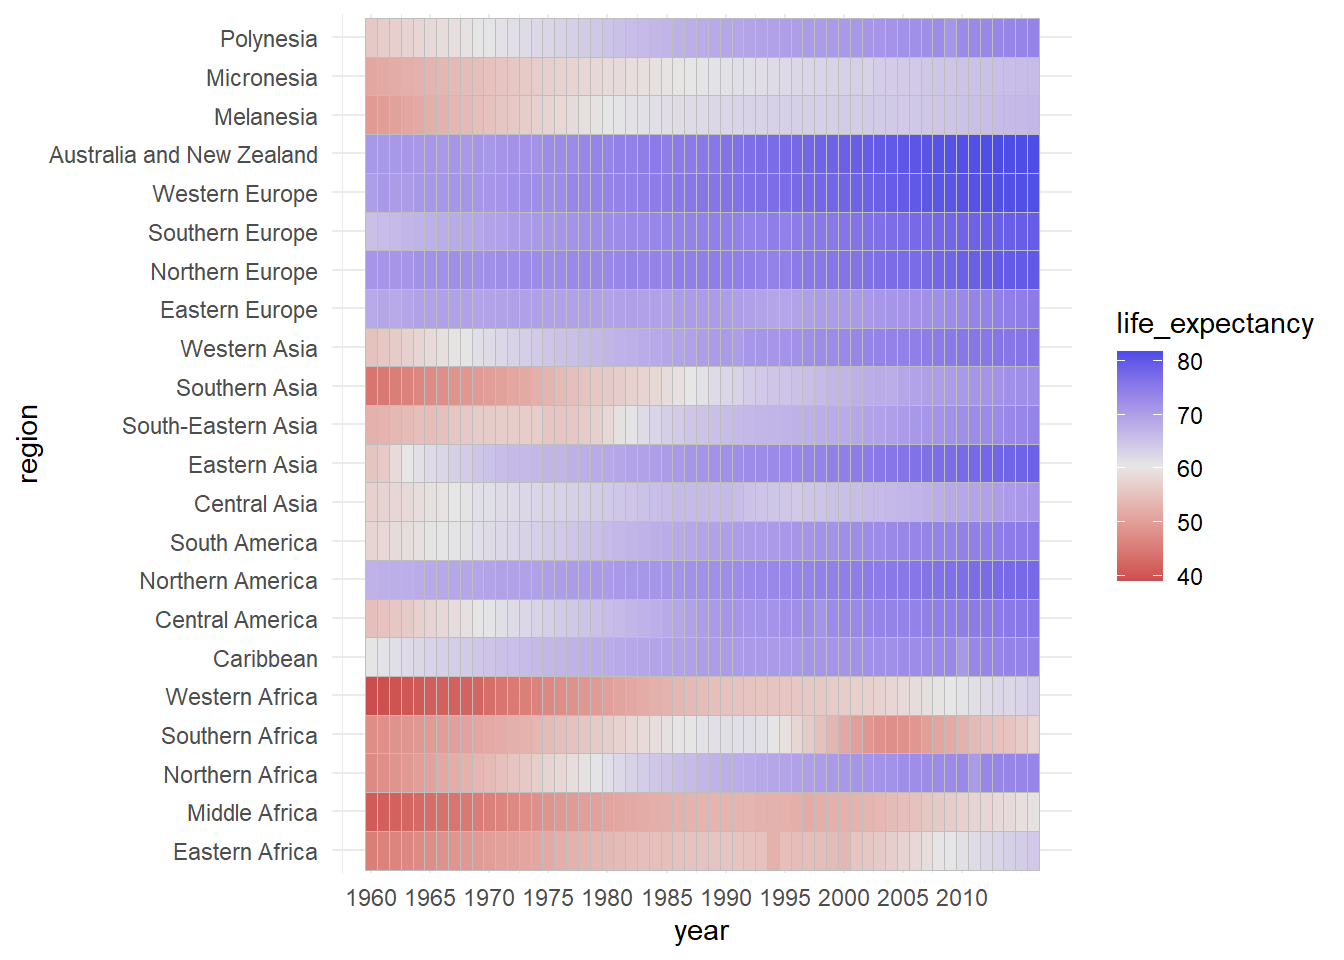
\includegraphics{02-literature_files/figure-latex/unnamed-chunk-8-1.pdf}

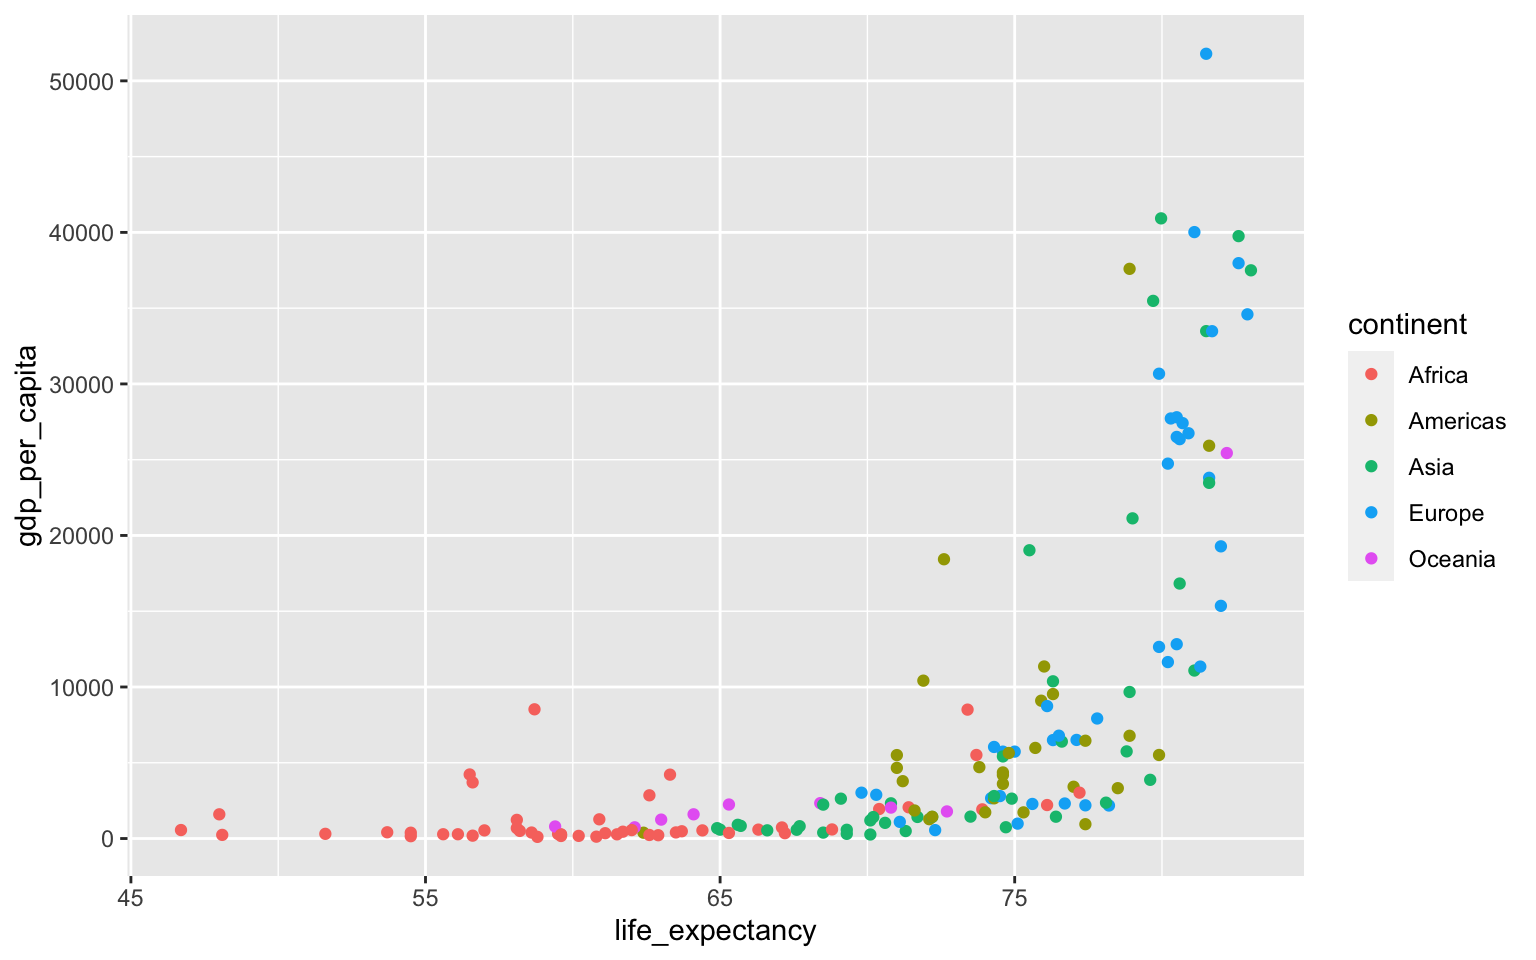
\includegraphics{02-literature_files/figure-latex/unnamed-chunk-9-1.pdf}

\hypertarget{ux111ux1ed9-chux1ec7ch-cux1ee7a-muxf4-huxecnh}{%
\subsubsection{Độ chệch của mô hình}\label{ux111ux1ed9-chux1ec7ch-cux1ee7a-muxf4-huxecnh}}

Ở một khía cạnh khác, độ chệch (bias) là từ được dùng để nhắc tới sai số được tạo ra khi ước lượng một vấn đề thực tế (có thể rất phức tạp), bằng một mô hình hàm \(\hat{f}\) đơn giản. Ví dụ, mô hình hồi quy tuyến tính thường giả định rằng có mối liên hệ tuyến tính giữa \(Y\) và các giá trị \(X_1, X_2, \cdot, X_p\). Tuy nhiên, hầu như không có hiện tượng nào trong thực tế đều có một mối quan hệ hồi quy tuyến tính hoàn toàn, vậy nên mô hình hồi quy tuyến tính sẽ luôn có độ chệch khi ước lượng hàm f.~Nhìn chung, phương pháp càng linh hoạt (more flexible) thường cho ra kết quả có độ chệch càng thấp.

\hypertarget{sux1ef1-ux111uxe1nh-ux111ux1ed5i-giux1eefa-ux111ux1ed9-chux1ec7ch-vuxe0-phux1b0ux1a1ng-sai-1}{%
\subsubsection{Sự đánh đổi giữa độ chệch và phương sai}\label{sux1ef1-ux111uxe1nh-ux111ux1ed5i-giux1eefa-ux111ux1ed9-chux1ec7ch-vuxe0-phux1b0ux1a1ng-sai-1}}

Sự đánh đổi này xuất hiện như một quy luật mà chúng ta cần phải nhớ, rằng khi chúng ta sử dụng những mô hình linh hoạt hơn, thì phương sai (variance) sẽ tăng và độ chệch (bias) sẽ giảm. Sự thay đổi của hai giá trị liên quan tới nhau, và sẽ xác định giá trị MSE của tập dữ liệu kiểm thử tăng hay giảm. Khi chúng ta tăng sự phức tạp (flexibility) của mô hình, độ chệch (bias) có xu hướng giảm nhanh hơn là phương sai (variance), dẫn đến giá trị kỳ vọng của MSE trên tập dữ liệu kiểm thử giảm. Tuy nhiên, đến một thời điểm nào đó, việc tăng sự phức tạp (flexibility) của mô hình chỉ giảm độ chệch (bias) đi một chút, nhưng lại làm tăng phương sai (variance) nhanh hơn nhiều, và kết quả là giá trị kỳ vọng của MSE trên tập dữ liệu kiểm thử tăng.

Mối liên hệ giữa độ chệch và phương sai khi thực hiện các mô hình học thống kê còn được gọi là sự đánh đổi giữa độ chệch và phương sai (bias-variance trade off). Thông thường, những phương pháp học thống kê cho ra hiệu quả cao trên tập dữ liệu kiểm thử thường là những phương pháp cho ra độ chệch thấp và phương sai thấp. Hiện tượng này được gọi là đánh đổi (trade off), bởi vì rất dễ để chúng ta có một mô hình với độ chệch thấp (low bias) và phương sai cao (high variance), hoặc một mô hình với độ chệch cao (high bias) và phương sai thấp (low variance). Vấn đề khó nhất là tìm ra phương pháp học thống kê nào mà cho ra được phương sai (variance) và độ chệch bình phương (squared bias) thấp nhất. Đó là mục tiêu chính của quyển sách này.

Trong những vấn đề thực tế, chúng ta không bao giờ quan sát được hàm f thật, vậy nên là nhìn chung chúng ta không thể tính ra giá trị MSE của tập dữ liệu kiểm thử, độ chệch (bias) và phương sai (variance) của một phương pháp học thống kê nào đó. Tuy nhiên, bạn đọc hãy luôn phải nhớ rằng có sự đánh đổi giữa độ chệch và phương sai (bias-variance trade off) trong các phương pháp thống kê. Trong quyển sách này, chúng tôi sẽ giới thiệucác phương pháp thống kê rất phức tạp (flexible) và có thể giúp chúng ta giảm rất nhiều độ chệch (bias). Tuy nhiên, điều đó, không có nghĩa rằng những phương pháp của chúng tôi sẽ tốt hơn những phương pháp đơn giản (hồi quy tuyến tính chẳng hạn). Một ví dụ đơn giản có thể chỉ ra như \ldots{}

Trong phần tiếp theo, tác giả sẽ giới thiệu về phương pháp cross-validation, là một cách để ước lượng giá trị MSE của tập dữ liệu kiểm thử trên tập dữ liệu huấn luyện, đây là một phương pháp rất hứa hẹn để xử lý các vấn đề liên quan đến sự đánh đổi giữa độ chệch (bias) và phương sai (variance).

\textbf{Tạo ra một tập dữ liệu nữa illustrate cái sự tăng và giảm MSE theo Bias và Variance này}

\hypertarget{sux1ef1-ux111uxe1nh-ux111ux1ed5i-giux1eefa-ux111ux1ed9-chux1ec7ch-vuxe0-phux1b0ux1a1ng-sai-cux1ee7a-phux1b0ux1a1ng-phuxe1p-k-fold-cross-validation}{%
\subsubsection{Sự đánh đổi giữa độ chệch và phương sai của phương pháp k-fold cross validation}\label{sux1ef1-ux111uxe1nh-ux111ux1ed5i-giux1eefa-ux111ux1ed9-chux1ec7ch-vuxe0-phux1b0ux1a1ng-sai-cux1ee7a-phux1b0ux1a1ng-phuxe1p-k-fold-cross-validation}}

Ở phần bên trên, chúng ta đã nói về việc phương pháp k-fold CV có lợi thế hơn phương pháp LOOCV về tốc độ tính toán do số phép tính mà phương pháp k-fold CV phải thực hiện là ít hơn. Ngoài lợi thế về tốc độ tính toán, phương pháp k-fold CV còn được ưa chuộng hơn bởi phương pháp này cho ra kết quả ước lượng sai số trên tập dữ liệu kiểm thử chính xác hơn phương pháp LOOCV. Đây là một ví dụ điển hình cho hiện tượng đánh đổi giữa độ chệch và phương sai của mô hình.

Như chúng ta đã nhắc đến ở phần trước (viết trang 205 nhưng trong quyển sách này chưa nhắc đến cái gì ở trước), phương pháp sử dụng tập dữ liệu xác thực (validation set approach) có xu hướng overestimate sai số trên tập dữ liệu kiểm thử, nghĩa là độ chệch sẽ tương đối lớn, bởi vì phương pháp này chỉ sử dụng một nửa lượng dữ liệu để ước lượng. Cùng với một logic đó, không khó để chúng ta nhận ra rằng phương pháp LOOCV sẽ cho ra một ước lượng gần như không chệch (approximately unbiased estimates) của sai số trên tập dữ liệu kiểm thử, bởi vì phương pháp LOOCV sử dụng n - 1 trên n quan sát trong dữ liệu, nghĩa là gần như toàn bộ dữ liệu chúng ta có. Khi chúng ta thực hiện phương pháp k-fold CV, giả sử với trường hợp k = 5 và k = 10, kết quả cho ra một mô hình với độ chệch nằm giữa hai phương pháp vừa liệt kê bên trên, do phương pháp này chỉ sử dụng \(\frac{(k-1)n}{k}\) quan sát cho tập dữ liệu huấn luyện, ít hơn phương pháp LOOCV nhưng nhiều hơn phương pháp sử dụng tập dữ liệu xác thực (validation set approach). Vậy nên, từ góc nhìn của các chuyên gia, nếu mục tiêu là làm giảm độ chệch, rõ ràng phương pháp LOOCV là phương pháp vượt trội hơn hẳn so với phương pháp k-fold CV.

Tuy nhiên, chúng ta đều biết rằng độ chệch không phải là mối quan tâm duy nhất trong quá trình chúng ta ước lượng mô hình; chúng ta cũng cần phải quan tâm đến cả phương sai của mô hình nữa. Những nghiên cứu cho thấy rằng phương pháp LOOCV có phương sai cao hơn phương pháp k-fold CV với k\textless n.~Tại sao lại như vậy? Khi chúng ta thực hiện phương pháp LOOCV, chúng ta thực ra đang tính trung bình sai số từ n mô hình ước lượng từ dữ liệu, và mỗi mô hình được huấn luyện trên một tập dữ liệu gần như y hệt nhau; điều này tạo ra những kết quả sai số có tương quan dương (highly positively correlated) lớn. Ở chiều ngược lại, khi chúng ta sử dụng phương pháp k-fold CV với k\textless n, chúng ta sẽ tính trung bình sai số của k mô hình ước lượng từ dữ liệu, nhưng các sai số này sẽ tương quan với nhau ít hơn, do các tập dữ liệu huấn luyện của k mô hình này ít trùng nhau hơn. Do trung bình của các phần tử có tương quan lớn sẽ có phương sai lớn hơn trung bình của các phần tử có tương quan nhỏ hơn, nên giá trị sai số trên tập dữ liệu kiểm thử từ phương pháp LOOCV sẽ có xu hướng cho ra phương sai lớn hơn là so với sai số trên tập dữ liệu kiểm thử từ phương pháp k-fold CV.

Tóm lại, chúng ta có sự đánh đổi giữa độ chệch và phương sai liên quan tới sự lựa chọn k trong k-fold CV. Từ những kết quả thực nghiệm trên rất nhiều dữ liệu, thường các chuyên gia xây dựng mô hình sẽ chọn thực hiện phương pháp k-fold CV với k = 5 hoặc k = 10, để tránh trường hợp sai số trên tập dữ liệu kiểm thử gặp phải tình trạng độ chệch quá cao hoặc phương sai quá cao.

\hypertarget{lux1edbp-buxe0i-touxe1n-phuxe2n-loux1ea1i}{%
\paragraph{Lớp bài toán phân loại}\label{lux1edbp-buxe0i-touxe1n-phuxe2n-loux1ea1i}}

Từ đầu quyển sách, chúng ta đã thảo luận về độ chính xác của mô hình trong lớp bài toán mô hình hồi quy. Tuy nhiên, rất nhiều thuật ngữ, phương pháp vừa được giới thiệu bên trên, ví dụ như sự đánh đổi giữa độ chệch và phương sai, cũng có thể được áp dụng cho lớp bài toán phân loại. Lớp bài toán phân loại có một sự khác biệt cơ bản với lớp bài toán hồi quy đó là biến phụ thuộc \(y_i\) của bài toán phân loại thường là biến định tính, còn biến \(y_i\) của lớp bài toán hồi quy là biến định lượng. Trong bài toán phân loại, giả sử chúng ta phải tìm hàm f dựa trên các quan sát \({(x_1, y_1),...,(x_n, y_n)}\), với \(y_1,...,y_n\) là giá trị định tính. Phương pháp đơn giản nhất để để đánh giá độ chính xác của hàm ước lượng \(\hat{f}\) là sử dụng tỷ lệ sai sót trên tập dữ liệu huấn luyện, được tính bằng công thức:

\begin{align*}
\text{Training Error Rate} = \dfrac{1}{n} \sum\limits_{i = 1}^{n} I(y_i \neq \hat{y_i})
\label{eq:trainerrorclass}
\end{align*}

Với \(\hat{y_i}\) là kết quả phân loại quan sát i sử dụng hàm \(\hat{f}\), và \(I(y_i \neq \hat{y_i})\) là biến phân loại nhận giá trị 1 nếu \(y_i \neq \hat{y_i}\) và 0 nếu \(y_i = \hat{y_i}\). Nếu I(\$y\_i \neq \hat{y_i}) = 0, có nghĩa là hàm \(\hat{f}\) đã phân loại chính xác quan sát thứ i, và bằng 1 nếu hàm \(\hat{f}\) phân loại sai quan sát thứu i. Công thức \eqref{eq:trainerrorclass} cho
thấy tỷ lệ sai sót trên tập dữ liệu huấn luyện bằng số quan sát bị phân loại sai chia cho tổng các quan sát được phân loại.

Biểu thức \eqref{eq:trainerrorclass} được gọi là tỷ lệ sai sót trên mô hình huấn luyện bởi vì giá trị sai số được tính trên dữ liệu được sử dụng để huấn luyện hàm \(\hat{f}\). Tương tự như lớp bài toán hồi quy, trong lớp bài toán phân loại chúng ta cũng quan tâm cả tỷ lệ những quan sát trên tập dữ liệu kiểm thử mà mô hình dự đoán sai. Tỷ lệ sai sót trên tập dữ liệu kiểm thử với các quan sát có dạng \{\((x_i, y_i\)\} (chú ý những dữ liệu trong tập dữ liệu kiểm thử phải khác tập dữ liệu huấn luyện) được cho bởi công thức:

\begin{align*}
\text{Test Error Rate} = \dfrac{1}{m} \sum\limits_{i = 1}^{m} I(y_i \neq \hat{y_i})
\label{eq:testerrorclass}
\end{align*}

Trong đó, \(\hat{y_m}\) là giá trị phân loại được gán cho quan sát thứ m, với các biến dự báo (predictors) \(x_m\), được xác định bởi hàm f.~Một hàm phân loại tốt là hàm cho giá trị biểu thức \eqref{eq:testerrorclass} nhỏ nhất.

\hypertarget{phuxe2n-loux1ea1i-bayes}{%
\paragraph{Phân loại Bayes}\label{phuxe2n-loux1ea1i-bayes}}

Ta có thể dễ dàng chứng minh (nhưng việc chứng minh nằm ngoài phạm vi của quyển sách này) rằng tỷ lệ sai sót trên tập dữ liệu kiểm thử trong công thức \eqref{eq:testerrorclass} là nhỏ nhất, bởi một hàm phân loại khá đơn giản với ý tưởng là gán cho mỗi quan sát giá trị có khả năng đúng nhất, dựa trên những biến dự báo (predictors) của quan sát đó. Nói cách khác, chúng ta sẽ gán cho quan sát \((x_m, y_m)\) trên dữ liệu kiểm thử với biến dự báo (predictors) \(x_m\) giá trị phân loại j nếu:

\begin{align*}
P(y_m = j|x_m)
\label{eq:bayesclassifier}
\end{align*}

là lớn nhất. Công thức \eqref{eq:bayesclassifier} là công thức xác suất có điều kiện, có nghĩa là xác suất mà \(y_m\) được phân loại thành loại j, với điều kiện các biến dự báo (predictors) là \(x_m\). Phương pháp phân loại này được gọi là phương pháp phân loại Bayes (Bayes classifier).

Phương pháp phân loại Bayes cho ra một trong những tỷ lệ sai sót trên tập dữ liệu kiểm thử thấp nhất có thể, được gọi là Bayes error rate. Thực tế, hàm phân loại Bayes luôn luôn chọn giá trị phân loại sao cho \eqref{eq:bayesclassifier} là lớn nhất, tỷ lệ sai sót sẽ là \(1 - max_{j}Pr(y_m = j|X = x_m)\) tại \(X = x_m\). Tổng quát hơn, ta có Bayes error rate được cho bởi công thức:

\begin{align*}
1 - E(\underbrace{max}_{j} Pr(Y = j|X))
\label{eq:bayeserrorrate}
\end{align*}

với ký hiệu E() thể hiện giá trị kỳ vọng trung bình của xác suất trên tất cả các giá trị có thể của X. Giá trị Bayes error rate này thường luôn lớn hơn 0, và chúng có giá trị khá tương đồng với sai số không thể giảm.

\hypertarget{k-nearest-neighbors}{%
\subparagraph{K-Nearest Neighbors}\label{k-nearest-neighbors}}

Trên lý thuyết, chúng ta luôn muốn dự đoán biến định tính sử dụng phương pháp Bayes. Tuy nhiên trong thực tế, dữ liệu của chúng ta không cho chúng ta biết phân phối của Y với điều kiện X, vậy nên chúng ta không thể tính toán hàm phân loại Bayes. Vậy nên, trong thế giới thống kê, hàm phân loại Bayes đóng vai trò như một tiêu chuẩn vàng không thể đạt tới, và người ta sẽ sử dụng phương pháp phân loại Bayes để so sánh với các phương pháp khác. Rất nhiều phương pháp đã được sử dụng để ước lượng \(P(Y|X)\) và sau đó cho gán cho quan sát phân loại được dự đoán có xác suất đúng cao nhất. Một trong những phương pháp đó là, phương pháp phân loại K-nearest neighbors (KNN). Phương pháp này được trình bày như sau: Cho một số dương K và một quan sát \(x_0\), hàm KNN trước tiên xác định K điểm trong trong tập dữ liệu huấn luyện gần với quan sát \(x_0\) nhất, gọi các điểm đó là \(N_0\). Tiếp đó, hàm KNN ước lượng giá trị xác suất có điều kiện của loại j bằng công thức sau:

\begin{align*}
P(Y = j|X = x_0) = \dfrac{1}{K} \sum\limits_{i \in N_0} I(y_i = j)
\label{eq:KNNclass}
\end{align*}

Ta có thể thấy rằng, xác suất có điều kiện của loại j trong công thức \eqref{eq:KNNclass} được tính bằng cách lấy số điểm trong \(N_0\) chia cho tổng số điểm trong dữ liệu, và sau đó hàm KNN phân loại quan sát \(x_0\) thành loại nhận giá trị xác suất lớn nhất trong công thức \eqref{eq:KNNclass}. Dù cho KNN là một phương pháp khá đơn giản, nhưng chúng lại thể hiện kết quả gần giống với phương pháp Bayes classifier một cách bất ngờ.

Tương tự với lớp bài toán hồi quy, trong lớp bài toán phân loại, chúng ta cũng không có mối liên hệ mạnh mẽ giữa sai số trên tập dữ liệu huấn luyện và sai số trên tập dữ liệu kiểm thử. Ví dụ với phương pháp KNN, nếu chúng ta cho K bằng 1, thì sai số trên tập dữ liệu huấn luyện sẽ bằng 0, nhưng sai số trên tập dữ liệu kiểm thử vẫn cao. Nhìn chung, nếu chúng ta sử dụng phương pháp phân loại linh hoạt (flexible) hơn, thì có khả năng sai số trên tập dữ liệu huấn luyện sẽ giảm, nhưng sai số trên tập dữ liệu kiểm thử vẫn tăng. Các phương pháp phân loại cũng gặp vấn đề về hiện tượng quá khớp và chưa khớp tương tự như các phương pháp hồi quy.

Tóm lại, trong cả lớp bài toán hồi quy và lớp bài toán phân loại, việc lựa chọn mức độ linh hoạt (flexibility) chính xác có vai trò tối quan trọng đến sự thành công của phương pháp học thống kê của chúng ta. Hiện tượng đánh đổi giữa độ chệch và phương sai khiến cho việc lựa chọn mức độ linh hoạt của mô hình trở nên khó khăn, tuy nhiên những phương pháp sử dụng dữ liệu xác thực và
đặc biệt là k-fold cross validation đã giải quyết phần nào vấn đề này.

\hypertarget{k-fold-cross-validation}{%
\subsection{K-fold cross validation}\label{k-fold-cross-validation}}

Ta lại đặt ra thêm một câu hỏi nữa, nếu như chúng ta không có dữ liệu kiểm thử thì chúng ta sẽ xây dựng mô hình như thế nào? Câu trả lời là sử dụng chính dữ liệu đào tạo để kiểm tra sự chính xác của mô hình. Tuy nhiên, chúng ta sẽ không sử dụng toàn bộ tập dữ liệu kiểm thử, mà chúng ta sẽ chia tập dữ liệu huấn luyện thành k phần khác nhau. Sau đó, chúng ta sẽ xây dựng mô hình trên k-1 tập dữ liệu huấn luyện con, và sử dụng tập dữ liệu huấn luyện con còn lại (thường gọi là tập dữ liệu xác thực) để kiểm tra sự chính xác của mô hình được xây dựng trên k-1 tập dữ liệu huấn luyện kia. Quá trình này được lặp lại k lần, để bất kỳ phần nào của tập dữ liệu huấn luyện cũng đều được làm tập dữ liệu xác thực. Cuối cùng, chúng ta tính trung bình của sai số trên toàn bộ các tập dữ liệu xác thực và so sánh. Mô hình nào cho giá trị trung bình sai số trên các tập xác thực khác nhau này nhỏ nhất thì sẽ là mô hình được chúng ta chọn. Phương pháp này thường được gọi là k-fold cross validation.

Diễn giải một cách toán học, giả sử thước đo cho sai số của chúng ta là MSE, và chúng ta có k ước lượng của sai số trên tập dữ liệu xác thực, lần lượt là \(MSE_1, MSE_2, MSE_3, ... , MSE_k\). Khi đó ước lượng giá trị k-fold cross validation sẽ được tính bằng công thức:

\begin{align}
CV_{(k)} = \dfrac{1}{k} \sum\limits_{i=1}^{k} MSE_i
\end{align}

Khi ta để giá trị k bằng với số các quan sát trong dữ liệu, khi đó ta sẽ có n tập dữ liệu xác thực, mỗi tập có duy nhất một quan sát. Trường hợp này gọi là Leave-one-out cross validation (LOOCV) và công thức ước lượng giá trị LOOCV trong trường hợp này là

\begin{align}
CV_{(n)} = \dfrac{1}{n} \sum\limits_{i=1}^{n} MSE_i
\end{align}

Hiện giờ quyển sách này đang giới thiệu hai phương pháp để tính toán giá trị cross-validation, vậy ưu và nhược điểm của hai phương pháp này là gì, và chúng ta sử dụng hai phương pháp này như thế nào trong phù hợp? Trong thực tế, để có thể tính toán ra được những con số này yêu cầu chúng ta phải thực hiện bằng máy tính, và đối với những bộ dữ liệu lớn thì tốc độ tính toán là hết sức quan trọng. Phương pháp LOOCV yêu cầu thuật mô hình thống kê của chúng ta phải chạy n lần, và điều này khả năng gây ra gánh nặng rất lớn về mặt tính toán (trừ trường hợp ta sử dụng mô hình ước lượng bình phương tối thiểu, có công thức tính nhanh chính xác là \(CV_{(n)} = \dfrac{1}{n} \sum\limits_{i=1}^{n} \left(\dfrac{y_i - \hat{y_i}}{1 - h_i}\right)^2\).
Phương pháp cross-validation là phương pháp được áp dụng rất rộng rãi, phù hợp hầu như với bất kỳ các mô hình thống kê đã biết. Trong những phương pháp đó, có những phương pháp yêu cầu cách tính toán rất phức tạp chứ không đơn giản như phương pháp ước lượng bình phương tối thiểu, và nếu như sử dụng LOOCV thì máy tính sẽ xử lý mất thời gian hơn rất nhiều, đặc biệt là nếu số lượng quan sát trong dữ liệu lớn. Ngược lại, việc thực hiện k-fold cross validation (thường là với k = 8 hoặc k = 10) thì quá trình xây dựng mô hình thống kê sẽ chỉ phải thực hiện 8 - 10 lần, điều này là khả thi hơn nếu lương dữ liệu được sử dụng lớn.

Ngoài lợi thế về mặt tính toán, phương pháp k-fold cross validation còn có một ưu điêm vượt trội nữa so với các phương pháp khác, nằm ở sự đánh đổi giữa bias và variance (bias-variance trade off). Phương pháp k-fold cross validation sẽ cho ra kết quả ước lượng của sai số trên tập dữ liệu kiểm thử chính xác hơn so với phương pháp LOOCV. Chúng ta đã từng nhắc đến việc phương pháp chọn mô hình dựa trên tập dữ liệu xác thực (validation test) có thể overestimate sai số trên tập dữ liệu kiểm thử, khi mà phương pháp này chỉ sử dụng lượng dữ liệu huấn luyện bằng khoảng một nửa tổng dữ liệu chúng ta có. Với logic này, rất đơn giản để chúng ta nhận ra rằng phương pháp LOOCV sẽ cho ra ước lượng gần như không chệch (approximately unbiased estimates) của tập dữ liệu kiểm thử, khi mỗi tập dữ liệu huấn luyện có tới n - 1 quan sát (tổng số quan sát trong dữ liệu là n). Tương tự, khi chúng ta chạy mô hình và sử dụng phương pháp k-fold cross validation (với các giá trị k khá nhau, có thể là k = 5 hoặc k = 10), chúng ta sẽ có được mức độ chệch vừa phải đối với sai số trên tập dữ liệu kiểm thử, vì khi đó mỗi tập dữ liệu huấn luyện sẽ có khoảng \(\dfrac{(k-1)n}{k}\) quan sát, ít hơn so với phương pháp LOOCV nhưng lại nhiều hơn phương pháp chỉ sử dụng một dữ liệu xác thực. Vậy nên, đứng trên góc độ của một người ưu tiên giảm độ chệch của ước lượng, rõ ràng phương pháp LOOCV được ưa chuộng hơn só với phương pháp k-fold cross validation.

Tuy nhiên, giảm độ chệch của ước lượng không phải là tất cả những gì chúng ta quan tâm khi ước lượng một mô hình. Một yếu tố rất quan trọng nữa mà chúng ta phải quan tâm đó là phương sai (variance) của mô hình. Nếu như so sánh về phương sai, phương pháp LOOCV hay k-fold cross validation sẽ cho ra kết quả tốt hơn? Câu trả lời là phương pháp k-fold cross validation (với điều kiện k\textless n). Lý do là vì khi chúng ta thực hiện phương pháp LOOCV, thực tế chúng ta đang tính trung bình các kết quả của n mô hình ước lượng, nhưng mỗi mô hình đều được huấn luyện dựa trên một tập dữ liệu gần như giống hệt nhau (chỉ khác nhau nhiều nhất là một quan sát); vậy nên, kết quả ước lượng của các mô hình thường có mối tương quan dương rất cao. Ngược lại, phương pháp k-fold cross validation (với điều kiện k \textless{} n) sẽ cho ra giá trị trung bình của kết quả của k mô hình ước lượng, và mức độ tương quan của các kết quả này sẽ ít hơn so với phương pháp LOOCV, vì số lượng các quan sát trùng nhau ở tập dữ liệu huấn luyện là nhỏ hơn. Bởi vì khi so sánh các chỉ số, thì giá trị trung bình của các chỉ số có mối tương quan cao sẽ luôn có phương sai cao hơn giá trị trung bình của các chỉ số có mối tương quan thấp, vậy nên là ước lượng sai số trên tập dữ liệu kiểm thử của phương pháp LOOCV có phương sai cao hơn so với phương pháp k-fold cross validation.

Tóm lại, phương pháp k-fold cross validation sẽ thể hiện được sự cân bằng tốt giữa độ chệch và phương sai, nhưng sự cân bằng này liên quan đến việc lựa chọn tham số k. Theo như các kết quả thưucj nghiệm cho thấy, khi chúng ta chọn giá trị k = 5 hoặc k = 10, thì phương pháp k-fold cross validation sẽ cho ra được ước lượng sai số trên tập dữ liệu kiểm thử không gặp phải tình trạng độ chệch hoặc phương sai quá cao.
(đang viết đến trang 205). Chúng ta sẽ sử dụng một dữ liệu được sinh ngẫu nhiên để thể hiện sự vượt trội của phương pháp k -fold cross-validation. Lý do là bởi vì khi chúng ta sử dụng dữ liệu thực tế, chúng ta sẽ không biết giá trị MSE thật của tập dữ liệu kiểm thử là bao nhiêu, và điều đó sẽ gây khó khăn nếu như chúng ta muốn đánh giá độ chính xác ước lượng cross-validation của mô hình. Còn nếu như chúng ta sử dụng dữ liệu sinh ngẫu nhiên, chúng ta có thể tính được giá trị MSE thật của tập dữ liệu kiểm thử.

\textbf{We need to generate a simulation data to shows that k-fold cross validation is better than Leave-one-out-cross-validation}

\begin{Shaded}
\begin{Highlighting}[]
\CommentTok{\# \# Load necessary libraries}
\CommentTok{\# library(caret) \# For cross{-}validation}
\CommentTok{\# library(MASS)  \# For synthetic data generation}
\CommentTok{\# library(ggplot2) \# For visualization}
\CommentTok{\# }
\CommentTok{\# \# Step 1: Data Simulation}
\CommentTok{\# \# Generate a synthetic dataset}
\CommentTok{\# set.seed(123) \# Set seed for reproducibility}
\CommentTok{\# n \textless{}{-} 250 \# Number of observations}
\CommentTok{\# p \textless{}{-} 5 \# Number of predictors}
\CommentTok{\# X \textless{}{-} matrix(rnorm(n * p), nrow = n, ncol = p) \# Generate predictors}
\CommentTok{\# beta \textless{}{-} runif(p, {-}2, 2) \# Random coefficients}
\CommentTok{\# epsilon \textless{}{-} rnorm(n, 0, 1) \# Noise}
\CommentTok{\# y \textless{}{-} X \%*\% beta + epsilon \# Generate target variable}
\CommentTok{\# data \textless{}{-} as.data.frame(cbind(X, y))}
\CommentTok{\# }
\CommentTok{\# \# Step 2: Model Selection}
\CommentTok{\# \# Linear regression model for this simulation}
\CommentTok{\# model\_formula \textless{}{-} as.formula(paste("V1 \textasciitilde{}", paste("V", 2:(p+1), sep="", collapse="+")))}
\CommentTok{\# }
\CommentTok{\# \# Step 3: Cross{-}validation Implementations}
\CommentTok{\# \# k{-}fold cross{-}validation}
\CommentTok{\# set.seed(123)}
\CommentTok{\# k\_fold\_results \textless{}{-} train(model\_formula, data=data, method="lm",}
\CommentTok{\#                         trControl=trainControl(method="cv", number=10, }
\CommentTok{\#                                                savePredictions = TRUE))}
\CommentTok{\# }
\CommentTok{\# \# Leave{-}one{-}out cross{-}validation (LOOCV)}
\CommentTok{\# set.seed(123)}
\CommentTok{\# loocv\_results \textless{}{-} train(model\_formula, data=data, method="lm",}
\CommentTok{\#                        trControl=trainControl(method="LOOCV", }
\CommentTok{\#                                               savePredictions = TRUE))}
\CommentTok{\# }
\CommentTok{\# \# Step 4: Performance Comparison}
\CommentTok{\# \# Extracting RMSE from each fold/iteration}
\CommentTok{\# k\_fold\_rmse \textless{}{-} k\_fold\_results$resample$RMSE}
\CommentTok{\# }
\CommentTok{\# \# Variance of the RMSE}
\CommentTok{\# k\_fold\_variance \textless{}{-} var(k\_fold\_rmse)}
\CommentTok{\# }
\CommentTok{\# \# Comparing computational efficiency}
\CommentTok{\# k\_fold\_time \textless{}{-} k\_fold\_results$times$total}
\CommentTok{\# loocv\_time \textless{}{-} loocv\_results$times$total}
\CommentTok{\# }
\CommentTok{\# \# Step 5: Visualization and Interpretation}
\CommentTok{\# \# Plotting the distribution of RMSE for both methods}
\CommentTok{\# rmse\_data \textless{}{-} data.frame(Method = rep(c("K{-}Fold", "LOOCV"), each=nrow(data)),}
\CommentTok{\#                         RMSE = c(k\_fold\_rmse, rep(mean(loocv\_rmse), nrow(data))))}
\CommentTok{\# }
\CommentTok{\# ggplot(rmse\_data, aes(x=Method, y=RMSE, fill=Method)) +}
\CommentTok{\#   geom\_boxplot() +}
\CommentTok{\#   ggtitle("Distribution of RMSE for K{-}Fold vs LOOCV") +}
\CommentTok{\#   xlab("Cross{-}Validation Method") +}
\CommentTok{\#   ylab("RMSE") +}
\CommentTok{\#   theme\_minimal()}
\CommentTok{\# }
\CommentTok{\# \# Displaying computational times}
\CommentTok{\# print(paste("K{-}Fold Computational Time:", k\_fold\_time, "seconds"))}
\CommentTok{\# print(paste("LOOCV Computational Time:", loocv\_time, "seconds"))}
\CommentTok{\# }
\CommentTok{\# \# Conclusion: This script should help illustrate the differences in variance and}
\CommentTok{\# \# computational efficiency between k{-}fold and LOOCV cross{-}validation techniques.}
\end{Highlighting}
\end{Shaded}

Khi chúng ta xây dựng mô hình với sai số nhỏ nhất tính theo cross validation, mục tiêu của chúng ta là xác định xem phương pháp thống kê mà ta lựa chọn được kỳ vọng thể hiện tốt như thế nào trên các dữ liệu mới được đưa vào; trong trường hợp này, chúng ta quan tâm đến ước lượng thực tế (actual estimate) của trung bình bình phương sai số trên tập dữ liệu kiểm thử. Tuy nhiên, trong một vài trường hợp khác, có thể chúng ta chỉ đơn thuần quan tâm đến vị trí của điểm cực tiểu trên đường ước lượng trung bình bình phương sai số trên tập dữ liệu kiểm thử. Lý do là bởi vì chúng ta đang thực hiện cross-validation với một vài phương pháp thống kê khác nhau, hoặc là với một phương pháp thống kê nhưng có các mức độ linh hoạt (flexibility) khác nhau để tìm ra phương pháp có sai số trên dữ liệu kiểm thử thấp nhất trong các phương pháp được thử. Với mục đích này, vị trí trên đường sai số bình phương trung bình mang lại giá trị sai số bình phương trung bình nhỏ nhất được quan tâm hơn là giá trị của sai số bình phương trung bình đó.

\textbf{Lấy ví dụ đồ thị cho thấy rằng dù các mô hình cho ra test error khác nhau, thì correct level of flexibility cũng thường khá gần nhau}

\hypertarget{cross-validation-cho-lux1edbp-buxe0i-touxe1n-phuxe2n-loux1ea1i}{%
\subsection{Cross-validation cho lớp bài toán phân loại}\label{cross-validation-cho-lux1edbp-buxe0i-touxe1n-phuxe2n-loux1ea1i}}

Cross-validation không chỉ phù hợp với lớp bài toán hồi quy, phương pháp này còn rất phù hợp với lớp bài toán phân loại. Khác với lớp bài toán hồi quy, nơi mà người ta thường sử dụng MSE, MAE là giá trị đánh giá sai số trên tập dữ liệu kiểm thử, lớp bài toán phân loại sử dụng số lượng các quan sát bị phân loại sai khi áp dụng mô hình vào dữ liệu. Ví dụ, trong lớp bài toán phân loại, sai số LOOCV có dạng như sau:

\begin{align*}
CV_{(n)} = \dfrac{1}{n} \sum\limits_{i = 1}^{n} Err_i
\label{eq:class_cv}
\end{align*}

với \(Err_i = I(y_i \neq \hat{y_i})\). Sai số của phương pháp k-fold cross validation và phương pháp sử dụng tập dữ liệu xác thực cũng được tính tương tự như sai số LOOCV.

\hypertarget{phux1b0ux1a1ng-phuxe1p-bootstrap}{%
\subsection{Phương pháp Bootstrap}\label{phux1b0ux1a1ng-phuxe1p-bootstrap}}

Phương pháp Bootstrap là một phương pháp thống kê rất mạnh, được ứng dụng rộng rãi để lượng hoá sự không chắc chắn của một ước lượng hoặc một phương pháp học thống kê. Một ví dụ đơn giản của phương pháp bootstrap là để ước lượng sai số chuẩn (standard errors) của tham số trong mô hình hồi quy tuyến tính. Trong trường hợp hồi quy tuyến tính (linear regression) thông thường, phương pháp này thường không có ích lắm, khi hầu như mọi gói lệnh thống kê đã tự động tính ra ước lượng sai số chuẩn (standard errors). Tuy nhiên, sức mạnh của phương pháp bootstrap đến từ việc nó có thể dễ dàng được áp dụng với rất nhiều phương pháp học thống kê khác nhau, trong đó có cả những phương pháp mà việc đo phương sai (measure of variablitiy) là rất khó khăn, và không được tính sẵn bởi những gói lệnh thống kê.

Trong phần này, chúng ta sẽ miêu tả về các bước thực hiện quá trình lấy mẫu để thực hiện phương pháp bootstrap bằng một ví dụ đơn giản như sau:

\begin{itemize}
\tightlist
\item
  Bước 1: Chọn ngẫu nhiên một quan sát từ dữ liệu gốc vào dữ liệu mẫu.
\item
  Bước 2: Đưa lại quan sát được chọn ở bước 1 vào dữ liệu gốc.
\item
  Bước 3: Lặp lại bước 1 và bước 2 n lần (n là số lượng quan sát trong dữ liệu gốc), ta thu được dữ liệu mẫu có n quan sát.
\end{itemize}

Phương pháp boostrap thường cho chúng ta một kết quả ước lượng phù hợp cho phương sai của tham số hoặc một thước đo nào đó cho một tập dữ liệu. Ở đây, chúng ta sẽ tạm gọi giá trị tham số/thước đo cần được ước lượng phương sai là \(\hat{\theta}_n = g(X_1, ... , X_n)\), với \(X_i\) là giá trị của quan sát thứ i trong mẫu VÀ g() là hàm để tính tham số/thước đo từ mẫu.

Thuật toán ước lượng phương sai bằng phương pháp bootstrap có thể được trình bày như sau:

\begin{itemize}
\tightlist
\item
  Bước 1: Lấy ra các quan sát mẫu \(X_1^*, ... , X_n^*\), chúng ta tính \(\hat{\theta}_n^* = g(X_1^*, ... , X_n^*)\)
\item
  Bước 2: Lặp lại bước 1 B lần, chúng ta thu được các ước lượng \(\hat{\theta_{n,1}^*},...,\hat{\theta_{n,B}^*}\)
\item
  Bước 3: Tính

  \begin{center}
  \hat{s} = \sqrt{\dfrac{1}{B}\sum\limits_{j = 1}^B (\hat{\theta}_{n,j}^* - \bar{\theta})}
  \end{center}
\end{itemize}

với \(\bar{\theta} = \dfrac{1}{B} \sum\limits_{j = 1}^B \hat{\theta}_{n,j}^*\)

\begin{itemize}
\tightlist
\item
  Bước 4: Thu được kết quả \hat{s}.
\end{itemize}

Khi thoả mãn các điều kiện thông thường, chúng ta có \(\dfrac{s^2}{Var(\hat{\theta}_n)}\) hội tụ xác suất đến 1, khi n \(\rightarrow \infty\). Khi đó, giá trị \(\hat{s}^2\) được chứng minh xấp xỉ bằng phương sai của \hat{\theta}\_n.~Thông thường, giả sử ta tính ra giá trị \(\hat{s}\) bằng 0.15, chúng ta có thể nói rằng, chúng ta kỳ vọng \(\hat{\theta}\) sẽ cách \(\theta\) một khoảng bằng 0.15. Trong xấp xỉ này, chúng ta có hai nguồn gây ra sai số. Nguồn sai số đầu tiên đến từ việc n là hữu hạn, và sai số thứ hai đến từ việc B là hữu hạn. Chúng ta không thể thay đổi giá trị của n, nhưng chúng ta có thể thay đổi giá trị của B. Nếu chúng ta cho giá trị B đủ lớn (trong thực tế ta thường lấy B = 10000), chúng ta có thể bỏ qua sai số sinh ra do B là hữu hạn.

Khi đã tìm ra phương sai của tham số/thước đo cho tập dữ liệu, chúng ta có thể xác định khoảng tin cậy của tham số/thước đo đó theo các bước sau:

\begin{itemize}
\tightlist
\item
  Bước 1: Lấy ra các quan sát mẫu \(X_1^*, ... , X_n^*\), chúng ta tính \(\hat{\theta}_n^* = g(X_1^*, ... , X_n^*)\)
\item
  Bước 2: Lặp lại bước 1 B lần, chúng ta thu được các ước lượng \(\hat{\theta_{n,1}^*},...,\hat{\theta_{n,B}^*}\)
\item
  Bước 3: Ta tính giá trị:
  \begin{align*}
  \hat{F}(t) = \dfrac{1}{B} \sum\limits_{j = 1}^{B} I(\sqrt{n}(\hat{\theta}_{n,j}^* - \hat{\theta}_n) \leq t)
  \end{align*}
\item
  Bước 4: Sử dụng hàm \hat{F}(t), ta tính được khoảng tin cậy của \(\hat{\theta}_n\) theo công thức sau:
  \begin{align*}
  C_n = \left[ \hat{\theta}_n - \dfrac{t_{1- \alpha/2}}{\sqrt{n}}, \hat{\theta}_n - \dfrac{t_{\alpha/2}}{\sqrt{n}}  \right]
  \end{align*}
  với \(t_{\alpha/2} = \hat{F}^{-1}(\alpha/2)\) và \(t_{1 - \alpha/2} = \hat{F}^{-1}(1 - \alpha/2)\).
\item
  Bước 5: Trả kết quả \(C_n\), đây chính là khoảng tin cậy của tham số/thước đo được tính từ dữ liệu.
\end{itemize}

Điểm mạnh của phương pháp bootstrap nằm ở chỗ chúng ta có thể lấy được mẫu dữ liệu B lần (với B không giới hạn) để đánh giá độ chính xác của ước lượng \(\theta\). Có một phương pháp tương đương với cách chọn dữ liệu bootstrap, đó là chúng ta sinh ra B bộ dữ liệu mới khác nhau với các đặc điểm giống với dữ liệu thực tế. Tuy nhiên, với dữ liệu thực tế, chúng ta lại không thể sinh ra một tập mẫu mới từ dữ liệu gốc, vậy nên ta không thể sử dụng được phương pháp kể trên. Với mục tiêu đạt được giá trị \(\hat{s}\) tốt nhất, phương pháp bootstrap vẫn được đánh giá là một phương pháp cho kết quả chính xác, khả năng ứng dụng tốt với các loại mô hình khác nhau.

\end{document}
